\documentclass[12pt]{article}

\usepackage{amsmath,amssymb,amsfonts,amsbsy}
%\usepackage{cite}
\usepackage{graphicx}
\usepackage[margin=20mm]{geometry}
\usepackage{wrapfig}
\usepackage[pagewise,displaymath]{lineno}
\usepackage{subfig}
\usepackage{epsfig}
\usepackage{authblk}
\usepackage[d]{esvect}
\usepackage{calc}
\usepackage[colorlinks=false,bookmarks=false,pageanchor=true]{hyperref}
\usepackage{cite}
\usepackage{hyperref}
\usepackage{listings}

\lstset{ %
 % backgroundcolor=\color{white},   % choose the background color; you must add \usepackage{color} or \usepackage{xcolor}
 % basicstyle=\footnotesize,        % the size of the fonts that are used for the code
 % breakatwhitespace=false,         % sets if automatic breaks should only happen at whitespace
 breaklines=true,                 % sets automatic line breaking
 % captionpos=b,                    % sets the caption-position to bottom
 % commentstyle=\color{mygreen},    % comment style
 % deletekeywords={...},            % if you want to delete keywords from the given language
 % escapeinside={\%*}{*)},          % if you want to add LaTeX within your code
 % extendedchars=true,              % lets you use non-ASCII characters; for 8-bits encodings only, does not work with UTF-8
 frame=single,                    % adds a frame around the code
 keepspaces=true,                 % keeps spaces in text, useful for keeping indentation of code (possibly needs columns=flexible)
 % keywordstyle=\color{blue},       % keyword style
 % language=Octave,                 % the language of the code
 % morekeywords={*,...},            % if you want to add more keywords to the set
 % numbers=left,                    % where to put the line-numbers; possible values are (none, left, right)
 % numbersep=5pt,                   % how far the line-numbers are from the code
 % numberstyle=\tiny\color{mygray}, % the style that is used for the line-numbers
 % rulecolor=\color{black},         % if not set, the frame-color may be changed on line-breaks within not-black text (e.g. comments (green here))
 % showspaces=false,                % show spaces everywhere adding particular underscores; it overrides 'showstringspaces'
 % showstringspaces=false,          % underline spaces within strings only
 % showtabs=false,                  % show tabs within strings adding particular underscores
 % stepnumber=2,                    % the step between two line-numbers. If it's 1, each line will be numbered
%  stringstyle=\color{mymauve},     % string literal style
%  tabsize=2,                       % sets default tabsize to 2 spaces
%  title=\lstname                   % show the filename of files included with \lstinputlisting; also try caption instead of title
}

\newcommand{\missET}{\vv{\not{\!\!E}}_T}
\newcommand{\abs}[1]{\lvert#1\rvert}

\begin{document}

\setcounter{section}{0}
\setcounter{subsection}{0}
\setcounter{equation}{0}
\setcounter{figure}{0}
\setcounter{footnote}{0}
\setcounter{table}{0}

\title{Measurement of Vector Boson Asymmetry in Transversely Polarized $pp$
Collisions at RHIC}

\author{Salvatore Fazio\thanks{sfazio@bnl.gov}}
\author{Dmitri Smirnov\thanks{dsmirnov@bnl.gov}}

\affil{Physics Department, Brookhaven National Lab}
\date{\today\\v1.0}

\maketitle

\newpage
\tableofcontents 

\newpage
\linenumbers


\section{Introduction}
%{{{

The present study is the first attempt to measure the single spin asymmetry for weak bosons produced
in transversely polarized proton collisions at STAR by a complete reconstruction of the boson kinematics. 

Transversely polarized spin effects have been an extremely active topic among experiment and theory in the past years, because of their connection to transverse momentum dependent (TMD) distributions (leading to a multi-dimensional picture of the proton) and a possible test of the framework and the underlying theory of perturbative QCD. For a quantitative application of the TMD framework to transverse single-spin asymmetries measured in proton-proton collisions, the required two scales (typically $Q^{2}$ and $p_{T}$) are not well defined, excepted for Drell-Yan di-lepton (DY) and $W^{\pm}$/$Z^{0}$ boson production. DY has been at the center of attention for the non-universality test of the so-called Sivers TMD function, %it requires large integrated luminosities and efficient background reduction. The high mass of $W$-bosons naturally provides a hard $Q^{2}$ scale already and their transverse asymmetries can be directly applied to a global TMD analysis.
$f^{\perp}_{1T}$, which describes the correlation of parton transverse momentum with the transverse spin of the nucleon.  There is evidence of a quark Sivers effect in Semi-Inclusive Deep Inelastic Scattering (SIDIS) measurements where the quark Sivers function is associated with a final state effect from the gluon exchange between the struck quark and the target nucleon remnants. On the other hand, for the virtual photon production in the Drell-Yan process, the Sivers asymmetry appears in the initial state of the interaction. As a consequence, the quark Sivers functions are of opposite sign in SIDIS and in Drell-Yan
%
\begin{equation}
f^\text{SIDIS}_{q/h^\uparrow} (x, k_\perp) = - f^\text{DY}_{q/h^\uparrow} (x, k_\perp).
\end{equation}

The experimental test of this sign change is one of the open questions in hadronic physics, and can provide insights on the TMD factorization. While luminosities required for a meaningful measurement of asymmetries in Drell-Yan production are challenging, $W^{\pm}$ and $Z^{0}$ bosons production is equally sensitive to the predicted sign change and can be well measured at the STAR experiment.  The results can also provide essential input to study the new theoretical concept of evolution effects of transverse momentum dependent distribution functions, because of the high $Q^{2}$ in the $W^{\pm}$/$Z^{0}$ production due to the large boson mass. The STAR experiment at RHIC is currently the only place in the world where these effects can be tested.

The transverse single spin asymmetry, $A_N$, has been derived in~\cite{Kang:2009bp} and its parametrization is based on the fits to SIDIS data.
Predictions show that a transverse asymmetry solely calculated from the lepton decay is diluted~\cite{Kang:2009bp} if compared to the same asymmetry calculated directely from the produced boson. 
Thus, a full reconstruction of the produced boson kinematics is crucial for a meaningful measurement.
The present analysis is based on a data sample collected in the year 2011 at STAR using transversely polarized proton-proton collisions at the center-of-mass energy of $\sqrt{s}=500$~GeV, the total integrated luminosity is $L_{int} = 25$ pb$^{-1}$. In the present work we use this exploratory run to test the possibility of fully reconstructing the $W^{\pm}$ boson kinematics at STAR, using the lepton decay and all other particles in the recoil from the initial hard scattering. This analysis also includes a first look at $A_{N}$ in $Z^{0}$ production. 
%A proposed measurement with increased statistics in 2016 will be directly competitive with a Drell-Yan measurement in pion-proton scattering at CERN.

%The single spin asymmetry (SSA) $A_N$ for the $W$ bosons and the lepton $l$
%from the $W$ decay has been derived in \cite{Kang:2009bp}. It is
%parametrized based on the fits of SIDIS data and given as a function of
%direction and transverse momentum. For the case of $W$ we have:
%
%\begin{equation}
%A^W_N = A^W_N(y_W, \phi_W, q_T) \equiv A_N(y, \phi, p_T) = A_N(\Omega, p_T),
%\label{eq:asym_wboson}
%\end{equation}
%
%where $\Omega = \{y, \phi\}$ is simply used as a shorthand for the direction of
%the particle in the lab frame. Similarly, for the lepton the expectated
%asymmetry depends on the direction of the lepton and its transverse momentum:
%
%\begin{equation}
%A^l_N = A^l_N(\eta_l, \phi_l, p_T) \equiv A_N(y, \phi, p_T) = A_N(\Omega, p_T)
%\label{eq:asym_lepton}
%\end{equation}

%}}}

\section{Preliminary Sensitivity Studies}
%{{{

In 2011 transversely polarized proton-proton beams were brought into collisions
at STAR with a center of mass energy of $500~GeV$. In this regime the $W$ is
expected to have a relatively small $P_T$. 
%as confirmed by a Monte-Carlo simulation in Figure~\ref{fig:MC_W_Pt}. 
We use PYTHIA~6.8 to
simulate $W^\pm \to e^\pm \nu_e$ to the LO with unpolarized beams. Expected
kinematic distributions of the lepton coming from the $W$ decay is shown in
Figure~\ref{fig:MC_W_eta}.

%\begin{figure}[tbh]
%\begin{center}
%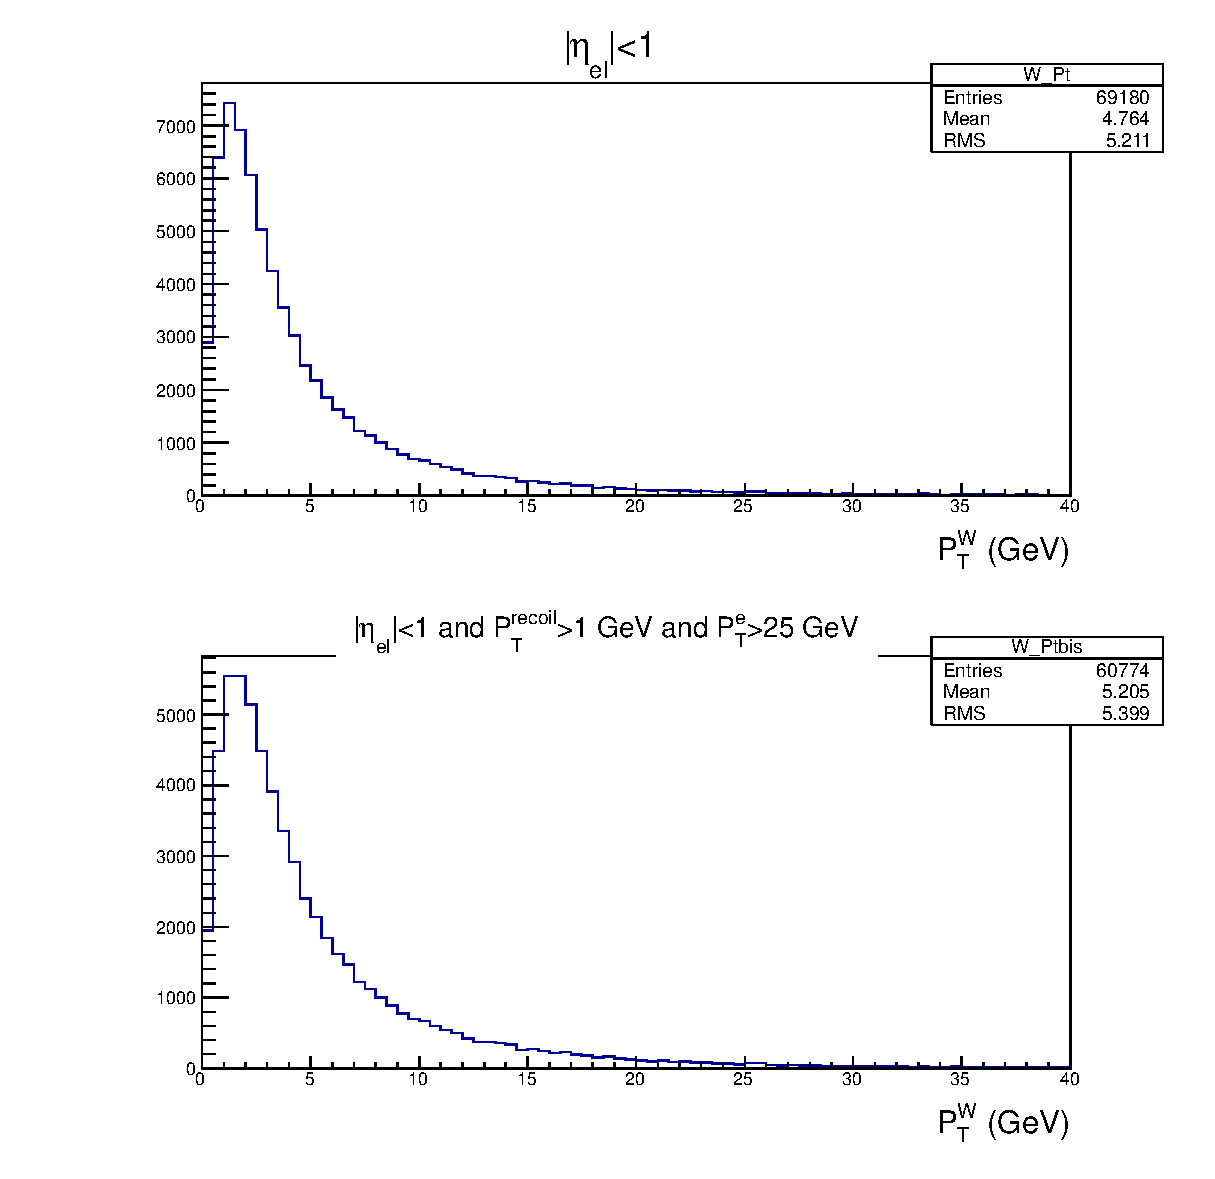
\includegraphics[width=10cm]{images/W_Pt}
%\end{center}
%\caption{Expected distribution of the transverse momentum of the produced W boson, $P^W_T$.}
%\label{fig:MC_W_Pt} 
%\end{figure}

\begin{figure}[htbp]
\begin{center}
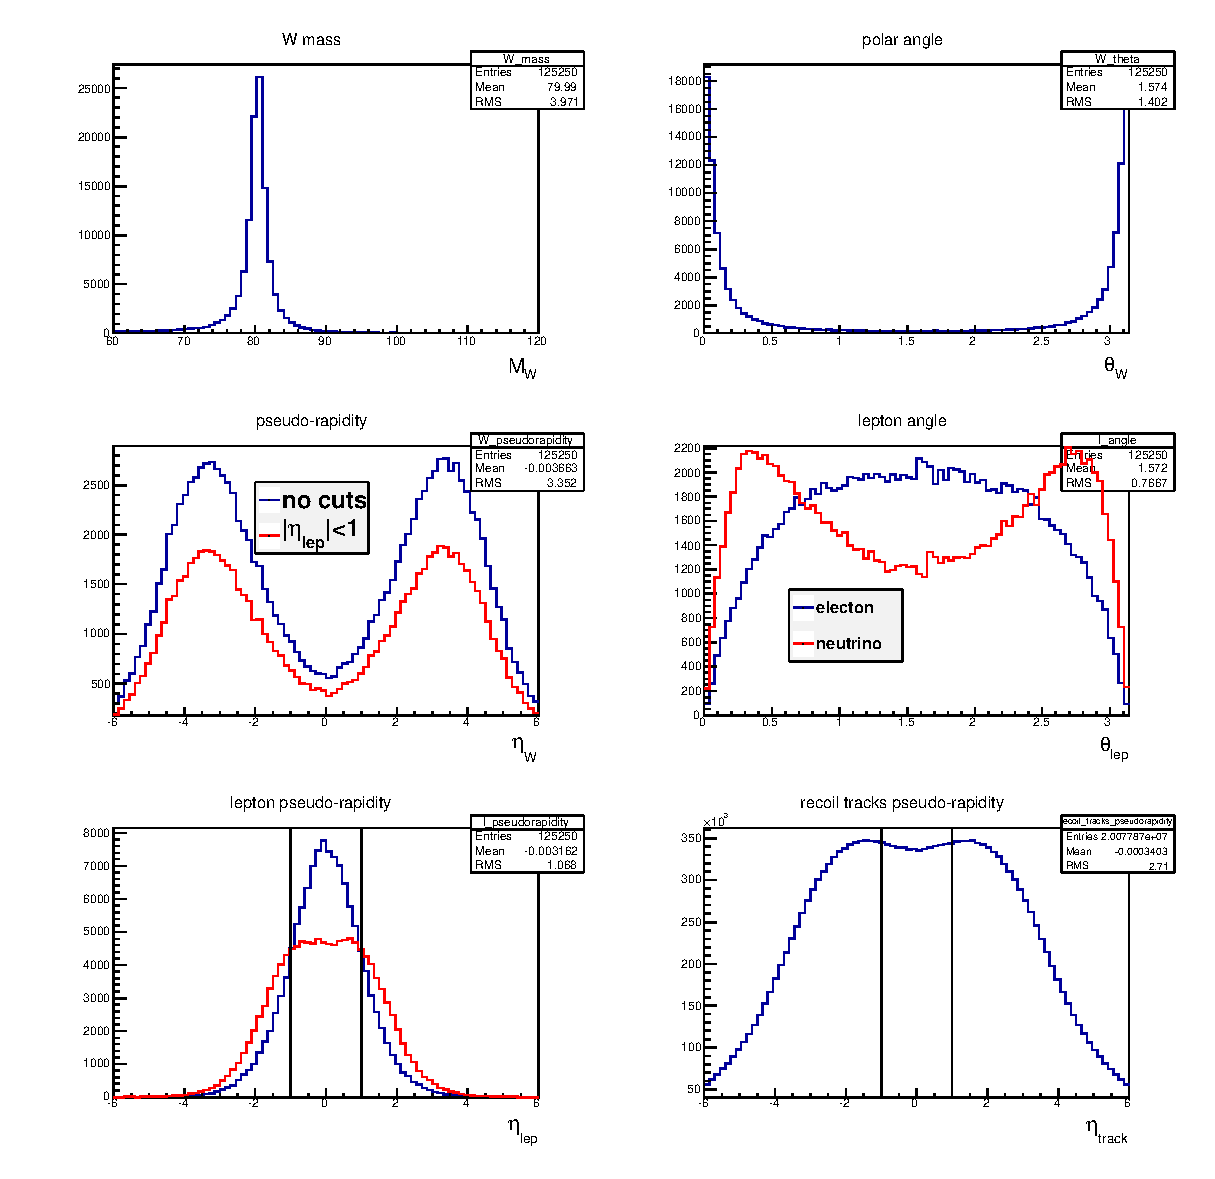
\includegraphics[width=14cm]{images/W_rapidity}
\end{center}
\caption{W-mass; polar angles and pseudo rapidity distributions of the produced W, the decay leptons and the recoil tracks.}
\label{fig:MC_W_eta} 
\end{figure}

%Most of the recoil tracks in the BARREL region are expected to carry a very
%small fraction of the energy as shown in fig.~\ref{fig:MC_recoil_Efrac}.

%\begin{figure}[htbp]
%\centering
%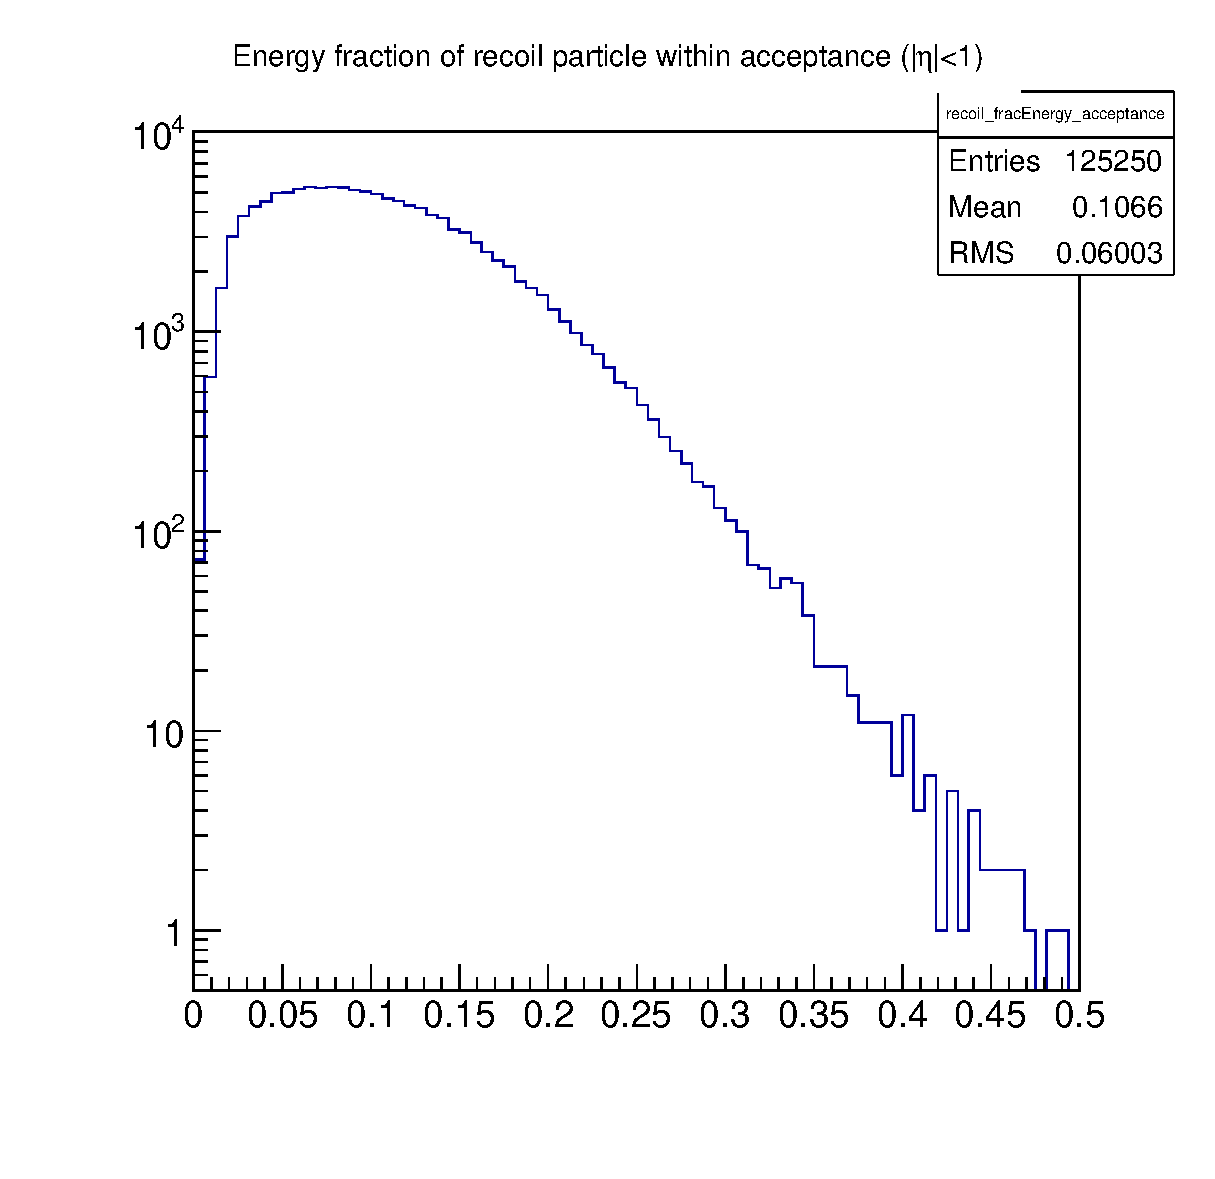
\includegraphics[height=0.25\textheight]{images/recoil_energy_frac.eps}
%\caption{Expected fraction of energy carried by recoil particles within the BARREL region ($|\eta|<1$).}
%\label{fig:MC_recoil_Efrac} 
%\end{figure}

Our aim is to use Monte Carlo to correct for the missing $P_{T}$ in the recoil tracks due to
the limited acceptance of the STAR detector. 
%\textit{Such a procedure will
%introduce a model-dependent systematic which has to be accounted for.} 
%which will grow with the value of the correction.}

%We estimate the statistical power of the $A_N$ measurement for an integrated
%luminosity of $300~\text{pb}^{-1}$. As a basis we use the total $W^\pm$ and
%$Z^0$ yields observed at STAR in Run 9. The $W$ and $Z$ candidate events,
%$N_\text{obs}$, along with the backgound numbers, $N_\text{bkg}$, are borrowed
%from the earlier STAR analysis~\cite{STAR_W_AL_2009-paper} that reported the production
%cross section using $\approx 13~\text{pb}^{-1}$ of inegrated luminosity:

%\begin{align*}
%N_{W^+} &= 496 - 37 = 459,\\
%N_{W^-} &= 148 - 26 = 125,\\
%N_Z &= 13 - 0 = 13.
%\end{align*}

%To reflect the expected increase in the integrated luminosity we scale the
%above numbers a factor $\approx 23$. In order to illustrate the sensitivity of
%the future measurement to the non-vanishing $W$ and $Z$ $A_N$ we calculate the
%relative yields in bins of the boson rapidity from the MC sample. The expected
%statistical power of $A_N$ in bins of $W$ rapidity is shown in
%Figure~\ref{fig:MC_Wmeas_stat} for $W^+$ and $W^-$ respectively compared with
%theoretical prediction from~\cite{Kang:2009bp}.

%\begin{figure}
%\subfloat[$W^+$]{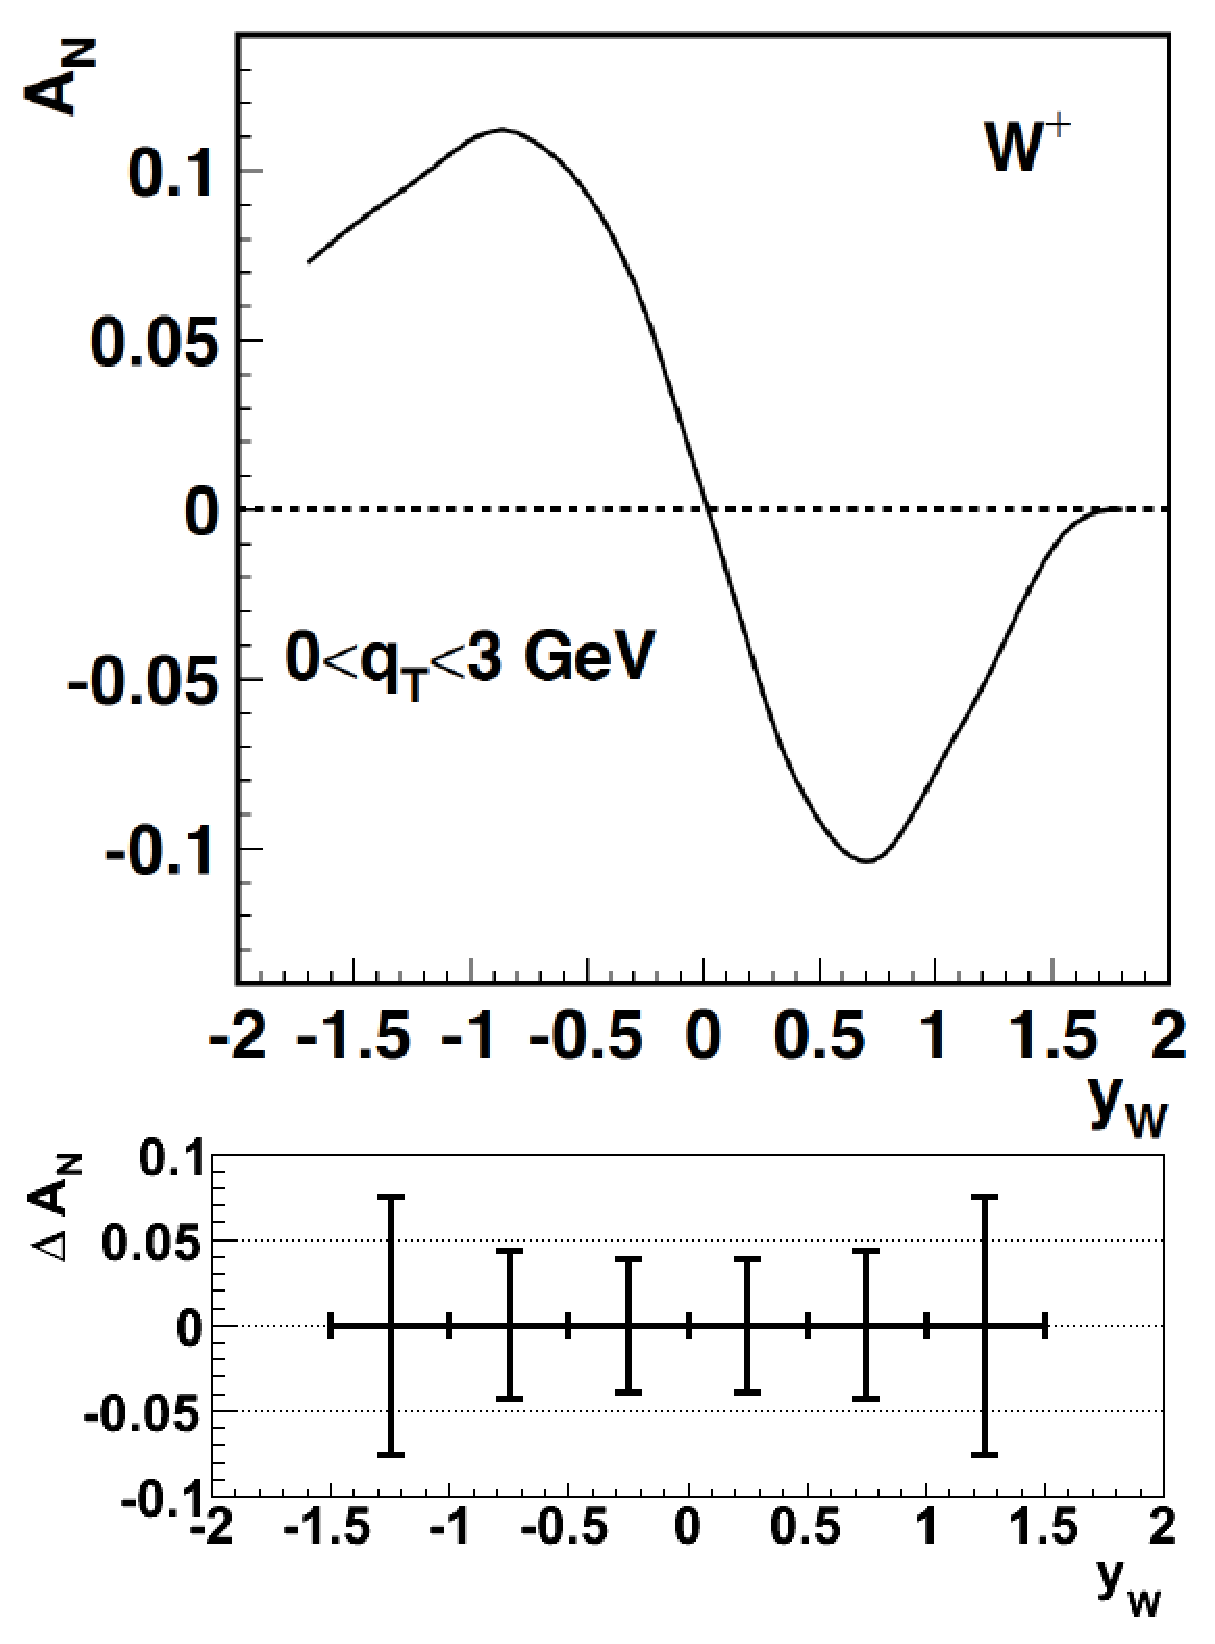
\includegraphics[width=0.49\textwidth]{images/anapow_w_plus} \label{fig:MC_Wmeas_stat_plus} }
%\subfloat[$W^-$]{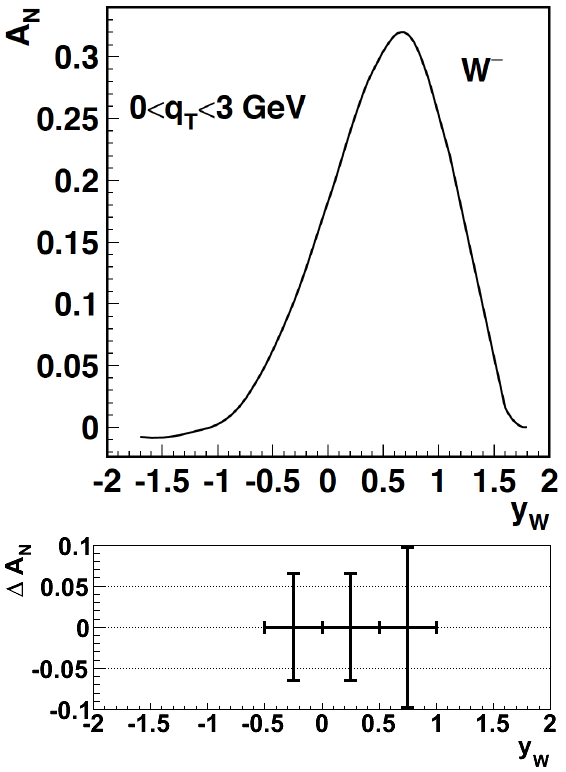
\includegraphics[width=0.49\textwidth]{images/anapow_w_minus}\label{fig:MC_Wmeas_stat_minus}}
%\caption[]{Expected statistical uncertainties for measured asymmetry $A_N$ of
%$W^+$ \subref{fig:MC_Wmeas_stat_plus} and $W^-$ \subref{fig:MC_Wmeas_stat_minus}
%decaying leptonically at STAR as a function of the boson's rapidity.}
%\label{fig:MC_Wmeas_stat} 
%\end{figure}

%}}}


\section{The $W^{\pm}$ selection and reconstruction}
\label{Wselection}
A data sample characterized by the $W$ signature has been selected, mostly requiring an isolated high $P_{T}$ electron and a hadronic recoil with a total $P_{T}$ sufficiently large. We adopt the same selection procedure already used (and described in details) at STAR for weak boson production measurements of polarized longitudinal single-spin asymmetry\cite{STAR_W_AL_2009-paper, STAR_W_AL_2009-note, STAR_W_AL_2012-paper, STAR_W_AL_2012-note} and unpolarized cross section\cite{STAR_W_xSec_2009-paper,STAR_W_xSec_2009-note}. The selection criteria are the following

\begin{itemize}
\item One isolated electron
    \begin{itemize}
    \item lepton-$P_{T}>25$~GeV;
    \item Track-$|\eta|<1$;
    \item Isolation criterium: $(P^{track}+E^{cluster})/\Sigma[P^{tracks}~\text{in R=0.7 cone]} > 0.8$;
    \item track coming from the maximum ranked vertex;
    \end{itemize}
\item $|Z_{vertex}| < 100$~cm; vertex rank $>$ 0;    
\item $P_{T}\text{-balance} > 15$~GeV, rejects QCD back ground;
\item $0.4 < |\text{Charge(TPC)}*E_{T}\text{(EMC)}/P_{T}\text{(TPC)}| < 1.8$, minimizes charge misidentification.
\end{itemize}

In the present analysis we also ask the total recoil-$P_{T} > 0.5$~GeV to minimize the systematics uncertainties in reconstructing the $W$ boson transverse momentum as described in Sec.~\ref{PT-reconstruction}.

%\begin{itemize}
%\item Total recoil-$P_{T} > 0.5$~GeV; 
%\item $P_{T}$ of each single track in the recoil $> 0.2$~GeV. 
%\end{itemize}
At the end we can identify two data samples depending on the electron charge; a positive charge identifies our $W^{+}$ signal whereas a negative charge marks our $W^{-}$ signal. After the whole selection procedure, the following events survive
\begin{itemize}
\item[--] positive-charged electron ($W^{+}$ signal): 1216 events;
\item[--] negative-charged electron ($W^{-}$ signal): 332 events.
\end{itemize}

%\subsection{$P_{T}$-balance requirement}
%$P_{T}\text{-balance} > 15$~GeV.
 
\subsection{Transverse momentum reconstruction} \label{PT-reconstruction}
In order to fully reconstruct the $W$ kinematics, the momenta of all $W$-decay
products must be measured. The momentum of the neutrino produced in the leptonically decayed $W$
cannot be measured and can only be indirectly deduced from momentum conservation. 
in the $W$ events produced at $\sqrt{s}=500$~GeV
at STAR we can assume that most of the missing energy, $\missET$ is carried by the neutrino from the
$W$ decay. The assumption ${P}_{\nu, T} \approx \missET$ is based on the
fact that only very little energy is left for anything other than $W$ production
from the primary hard scattering.
In the transverse plane the initial momentum of the system of interacting partons is negligible
and so must be the vector sum of all final particles momenta. We define the
missing transverse energy as a vector restoring the balance in the event:

\begin{equation}
\missET = - \sum_{i \in \parbox[t]{\widthof{\tiny clusters}}{\tiny tracks, clusters}} \vv P_{i,T}.
%miss ET = - \sum_{clusters}{jets, tracks, clusters} P_{i,T}.
\end{equation}

In a typical collider detector like STAR the problem with measuring the missing momentum from the hadronic recoil
is that particles with very high rapidities escape the detector. At the same time, the beam remnants with high
longitudinal momentum carry away only a little portion of the total transverse
momentum. We accounted for the non measured tracks and clusters by using the following event-by-event Monte Carlo 
correction to the data

\begin{equation}
k_{i}=\frac{P^{W}_{T,i}(true)}{P^{Recoil}_{T,i}(reconstructed)},
\end{equation}
where $P^{W}_{T,i}(true)$ is the generated $P_{T}$ of the $W$ at MC level and $P^{Recoil}_{T,i}(reconstructed)$ is the $P_{T}$ of the recoil reconstructed after a full GEANT simulation of the detector in each $i$-th bin. The distribution of the correction factor, $k$, versus the recoil $P_{T}$ is shown in Fig.~\ref{fig:plot_PtCorrFactor}. The correction has been applied to the data on an event-by-event base as follows

\begin{enumerate}
   \item read the $i$-th bin of recoil-$P_{T}$ from data;
   \item do a Y-Projection the correction factor from Fig.~\ref{fig:plot_PtCorrFactor} in the corresponding $i$-th bin;
   \item normalize the projection distribution to 1;
   \item use a random generator to select a correction value from the normalized projection distribution.
\end{enumerate}

A MC test shows that after the correction has been applied, data are in a very good agreement with predictions from RhicBOS and PYTHIA, as shown in Fig.~\ref{fig:plot_PtCorr}. In reconstructing the hadronic recoil from the tracks and clusters, additional cuts have been applied to avoid the very low total recoil-$P_{T}$, when most of the tracks fall off the STAR tracker (TPC) acceptance 
\begin{itemize}
   \item[--] Total recoil-$P_{T} > 0.5$~GeV; 
    \item[--] $P_{T}$ of each single track in the recoil $> 0.2$~GeV. 
\end{itemize}
Figure~\ref{fig:plot_DataMc_WpPt_PtRecoil} shows how the data/MC agreements improves requiring a minimum recoil-$P_{T}$ value of 0.5~GeV compared with a lower or no threshold.
The final data/MC agreement for reconstructing the $W$ boson transverse momentum over an extended range is  shown in Fig.~\ref{fig:plot_DataMc_Wp}($left$).


\begin{figure}[htbp]
\begin{center}
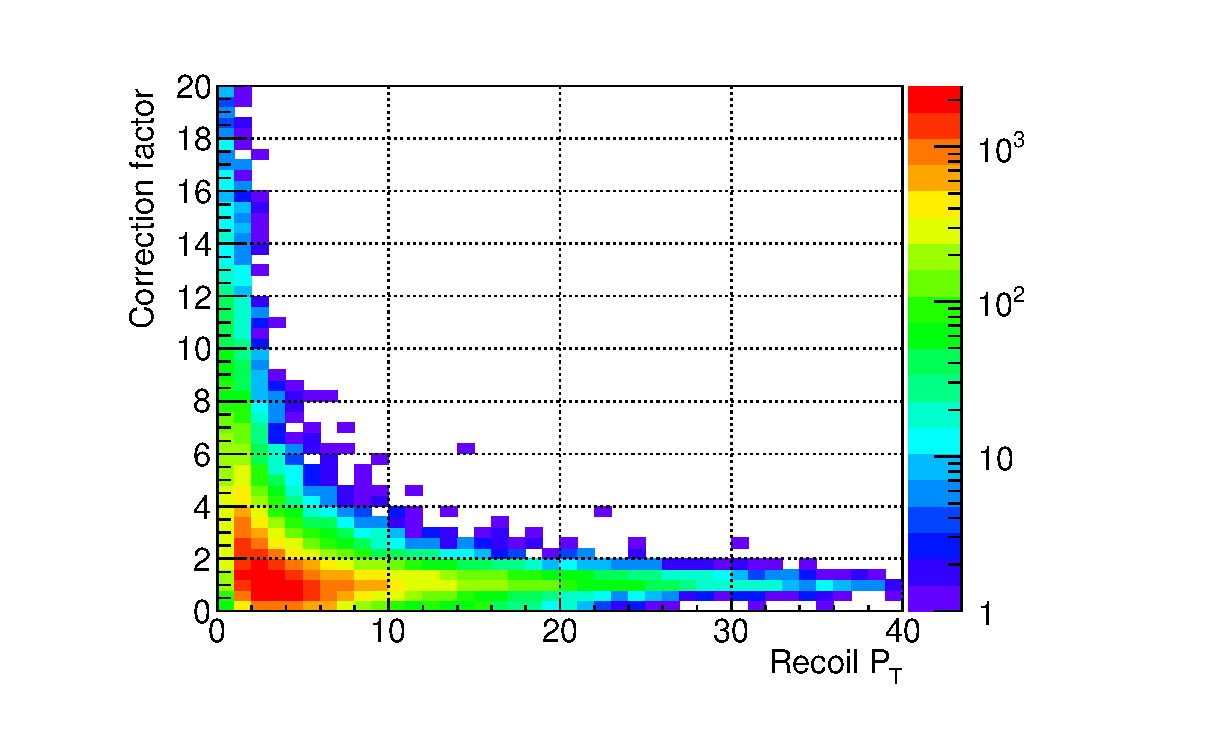
\includegraphics[scale=0.8]{images/plot_PtCorrFactor}
\end{center}
\caption{Distribution of the correction factor, $k$, versus the recoil $P_{T}$.}
\label{fig:plot_PtCorrFactor} 
\end{figure}

\begin{figure}[htbp]
\begin{center}
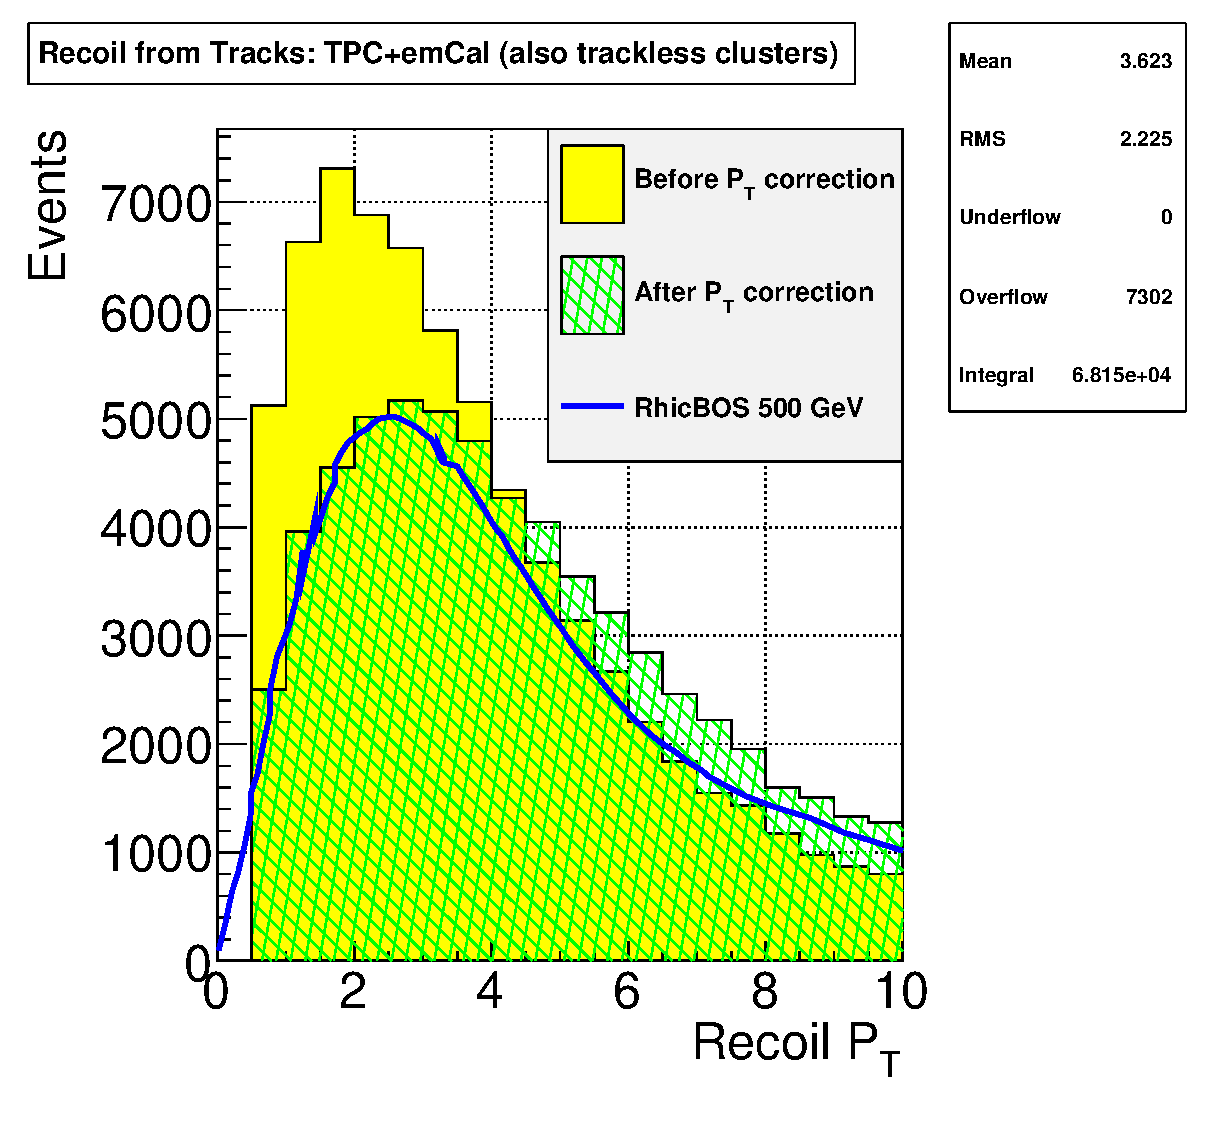
\includegraphics[scale=0.4]{images/plot_PtCorr}
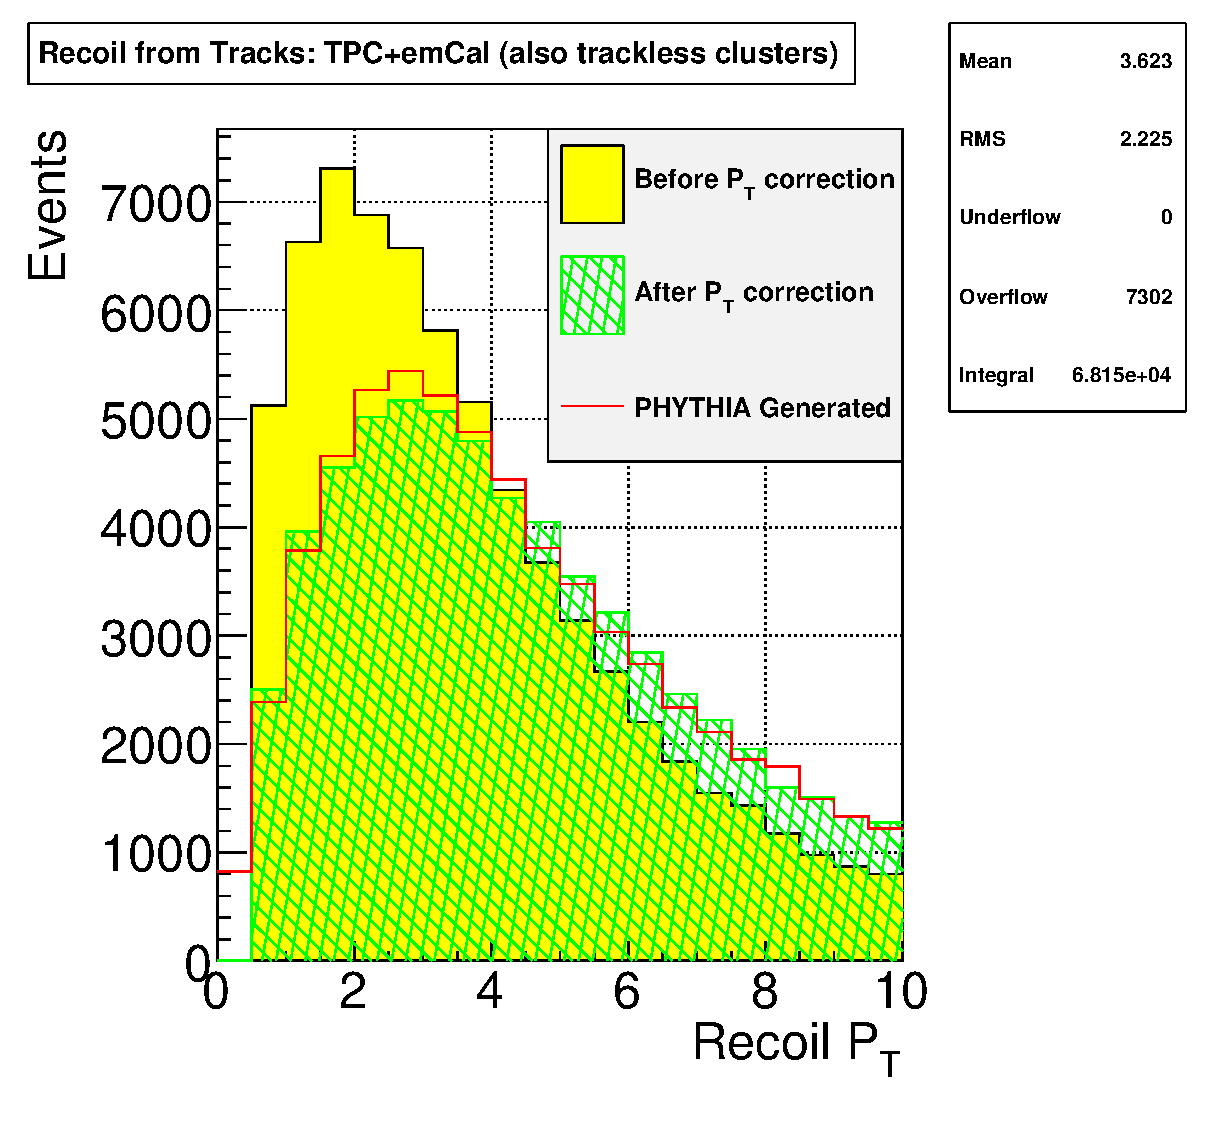
\includegraphics[scale=0.4]{images/plot_PtCorr2}
\end{center}
\caption{Data before and after the $P_{T}$ correction has been applied are compared with predictions from RhicBOS ({\it left}) and PYTHIA ({\it right}).}
\label{fig:plot_PtCorr} 
\end{figure}

\begin{figure}[htbp]
\begin{center}
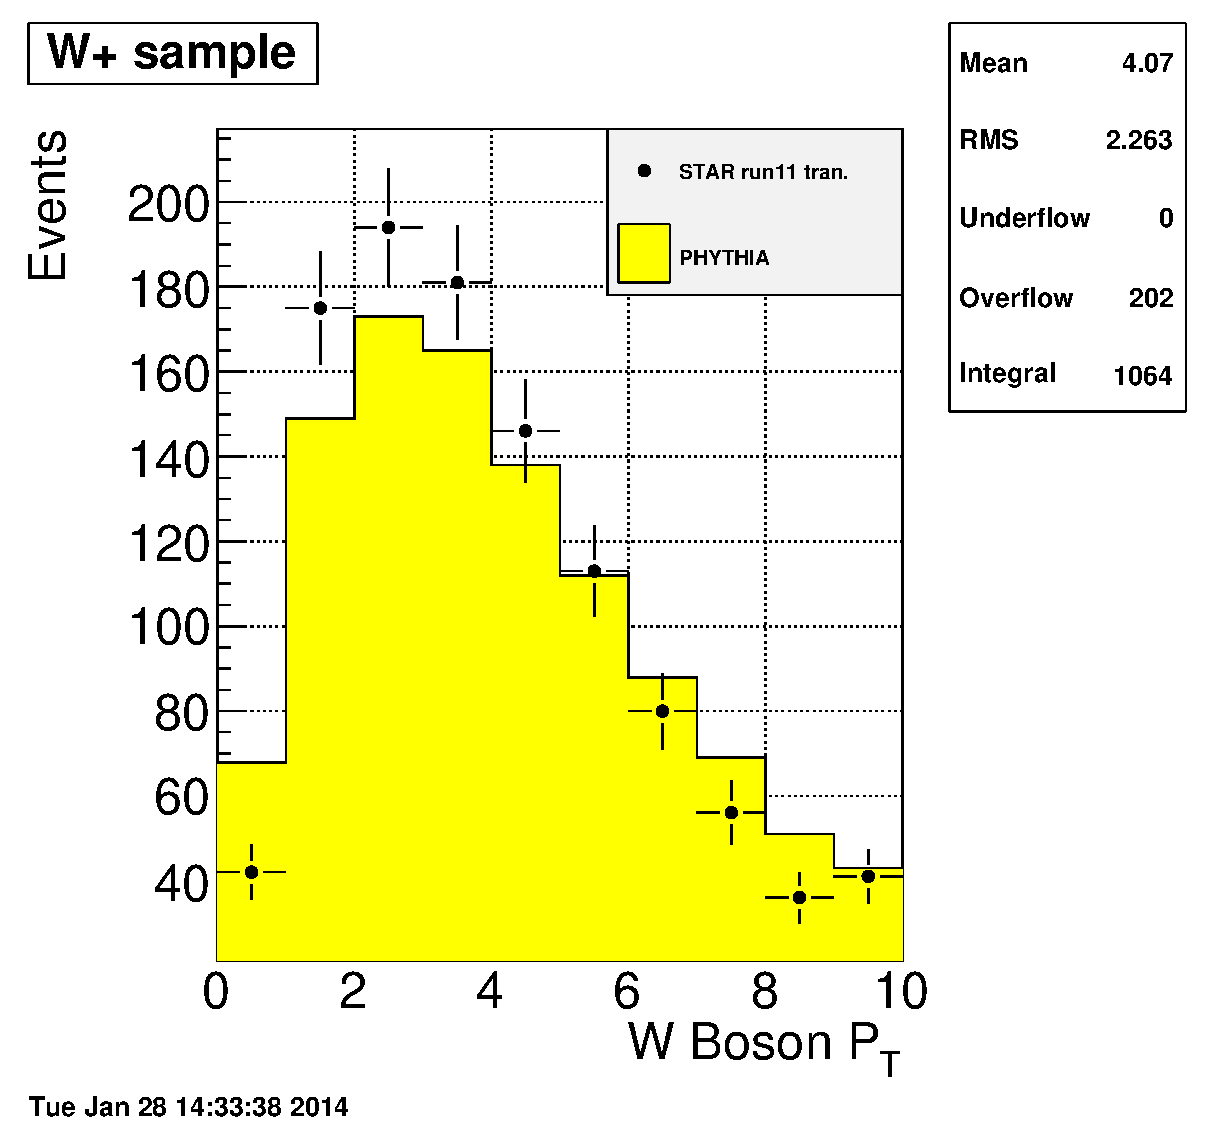
\includegraphics[scale=0.28]{images/Pt-Recoil-study/plot_DataMc_WpPt_PtRecoil02}
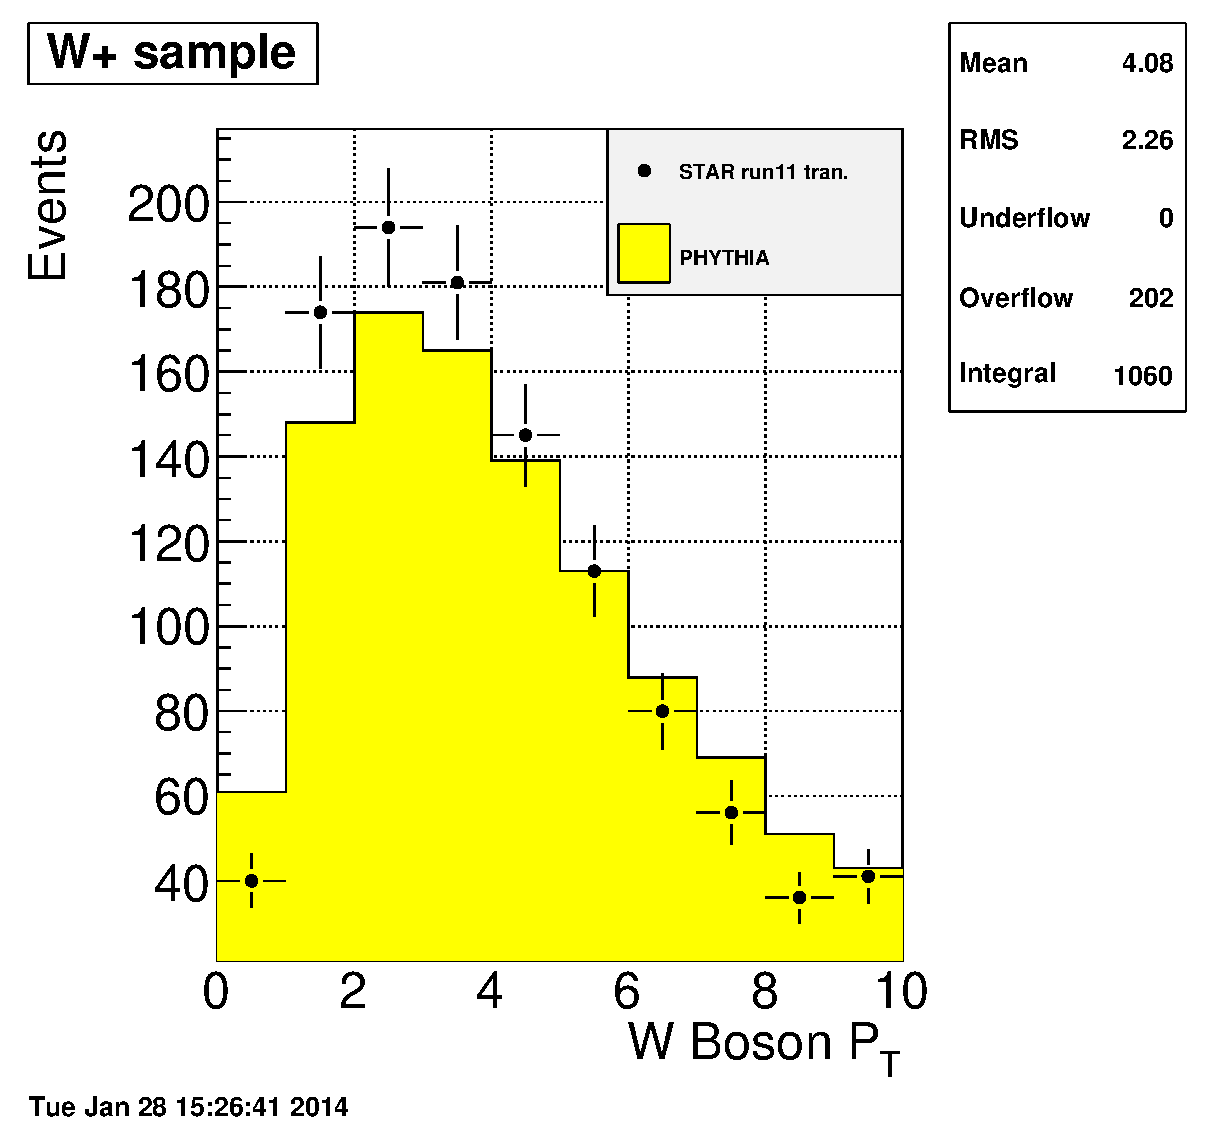
\includegraphics[scale=0.28]{images/Pt-Recoil-study/plot_DataMc_WpPt_PtRecoil03}
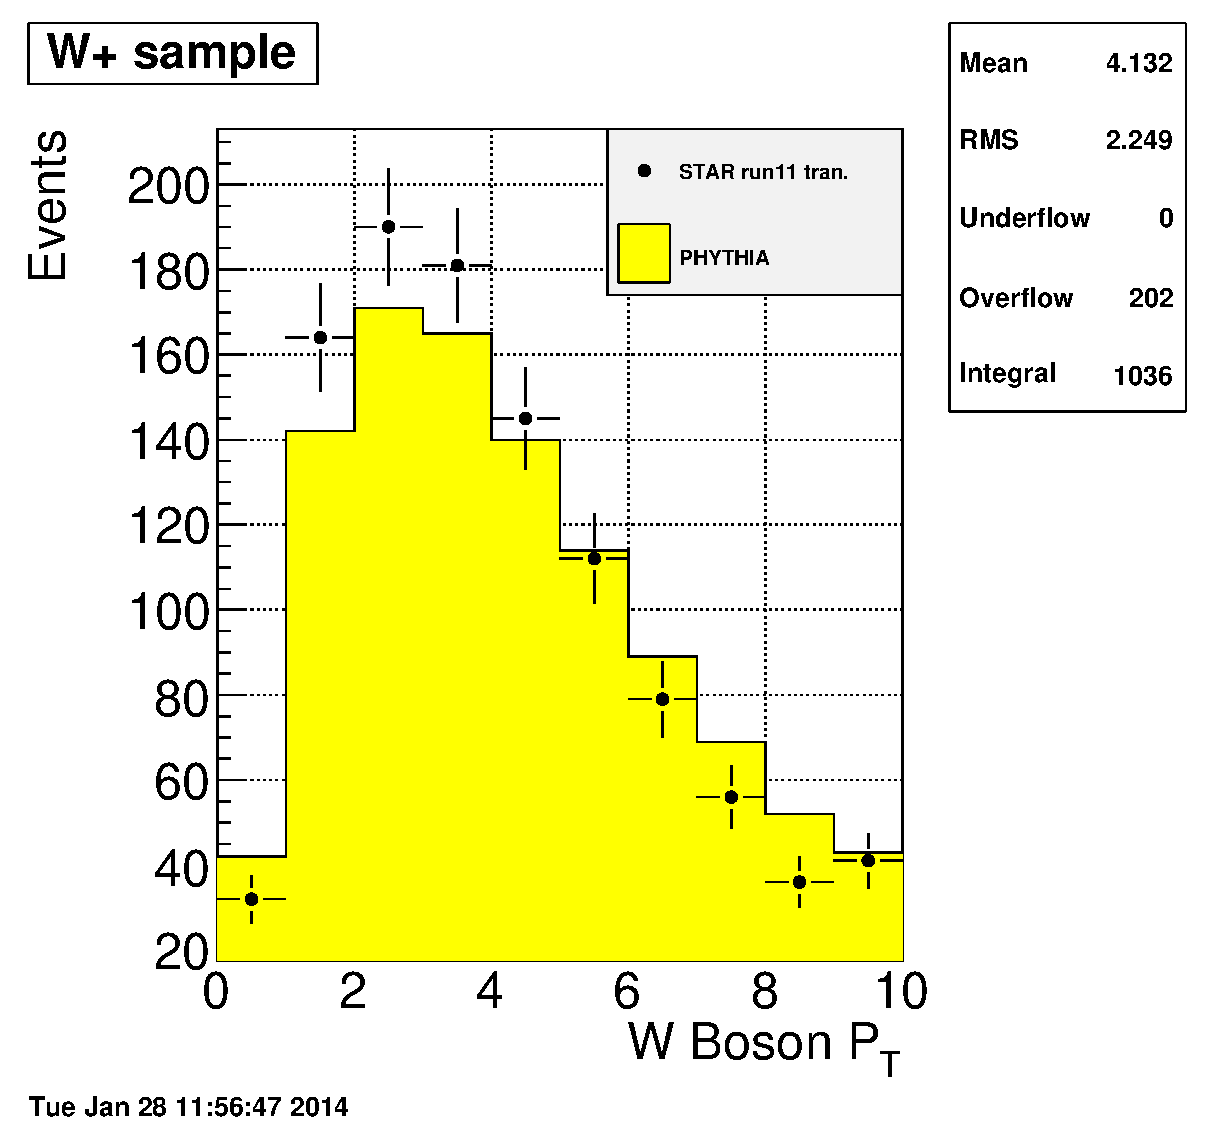
\includegraphics[scale=0.28]{images/Pt-Recoil-study/plot_DataMc_WpPt_PtRecoil05}
\end{center}
\caption{Data/MC agreement for the total recoil-$P_{T}$ with a minimum value of $P_{T}>0.2$~GeV ({\it left}), $P_{T}>0.3$~GeV ({\it center}) and $P_{T}>0.5$~GeV ({\it right}).}
\label{fig:plot_DataMc_WpPt_PtRecoil}
\end{figure}

\subsection{Longitudinal momentum reconstruction}
Knowing its transverse momentum, the longitudinal component of the neutrino's momentum can be reconstructed solving the quadratic equation for the invariant mass of the produced boson

\begin{equation}
\label{eq_InvMass}
M^{2}_{W}=(E_{e}+E_{\nu})^{2} - (\vv P_{e}+\vv P_{\nu})^{2},
\end{equation}
which leads to
\begin{equation}
M^2_W/2 = \abs{\vec{p}_l} \abs{\vec{p}_\nu} - \vec{p}_{l,T} \cdot \vec{p}_{\nu,T} - \vec{p}_{l,z} \cdot \vec{p}_{\nu,z},
\end{equation}
where we neglected the masses of the both neutino and lepton. Introducing a
shorthand expression for $A = M^2_W/2 + \vec{p}_{l,T} \cdot \vec{p}_{\nu,T}$,
after trivial arithmetics we arrive to a quadratic equation %for $p_{\nu,z}$

\begin{align}
\abs{\vec{p}_{l,T}}^2 p^2_{\nu,z} - 2A p_{l,z} p_{\nu,z} + \abs{\vec{p}_{\nu,T}}^2 \abs{\vec{p}_{l}}^2 - A^2 = 0.
\end{align}

In solving this equation we assumed the nominal value of the $W$-mass.  Thus, Eq.~\ref{eq_InvMass} leads to two possible solutions for the longitudinal component of the neutrino (and thus the $W$) momentum
\begin{align}
p_{\nu,z} = \frac{ A p_{l,z} \pm \sqrt{ A^2 p^2_{l,z} - \abs{\vec{p}_{l,T}}^2 (\abs{\vec{p}_{\nu,T}}^2 \abs{\vec{p}_{l}}^2 - A^2) } }{\abs{\vec{p}_{l,T}}^2}.
\end{align}

To distinguish between the two solutions, from now on we name ``first solution'' the one with the smaller absolute value and ``second solution'' the remnant one. In order to choose which solution should be used, the fraction of correctly reconstructed events for each solution was estimated via MC. The MC distribution of the reconstructed $P^{W}_{L}$ versus the generated level one is shown in Fig.~\ref{fig:plot_hRecoVsWBosonPz}  for both solutions separately. To estimate the amount of ``well reconstructed'' events we considered all the events with a reconstructed longitudinal moments within 30~GeV from the generated value (the to black limit-lines in  Fig.~\ref{fig:plot_hRecoVsWBosonPz}). The overall fraction of well reconstructed events, estimated according to this criterium, is shown for both solutions separately in the upper side of each plot in Fig.~\ref{fig:plot_hRecoVsWBosonPz}.
\begin{figure}[htbp]
\begin{center}
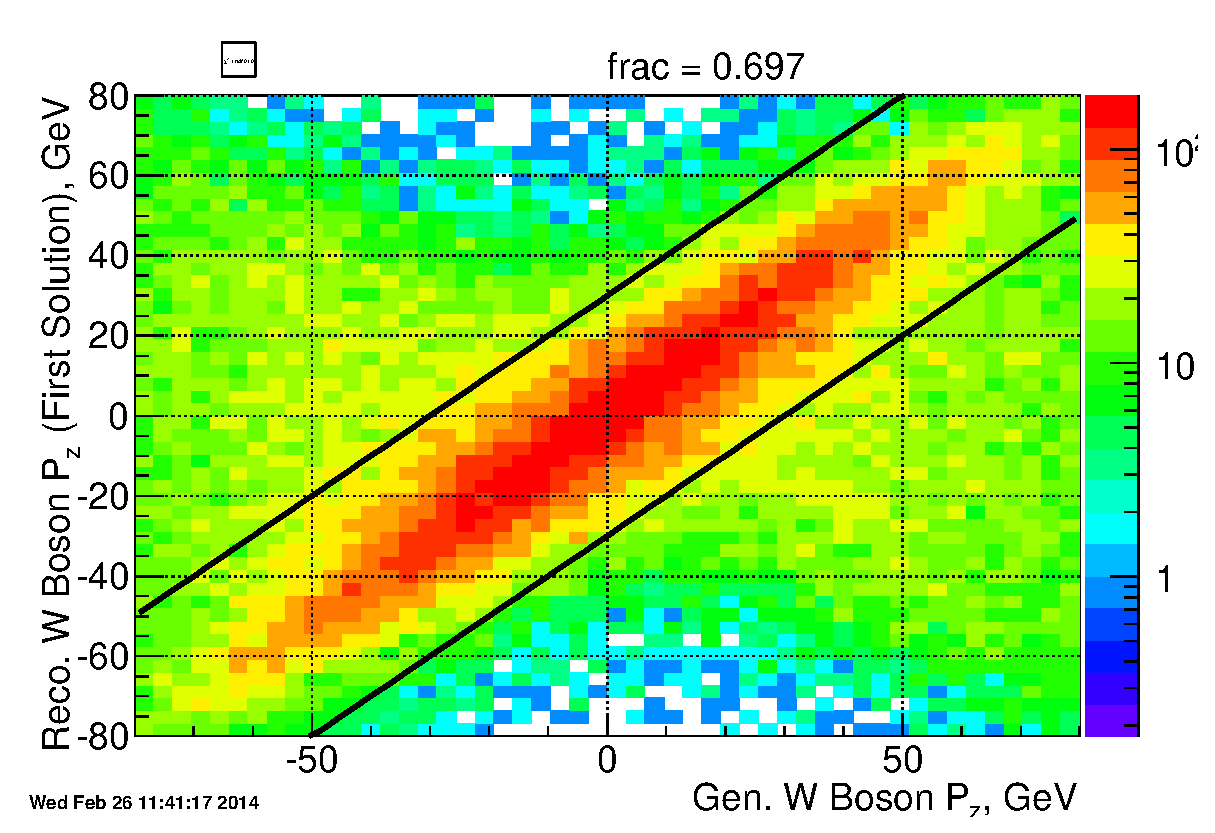
\includegraphics[scale=0.43]{images/P_long_study/hRecoVsWBosonPz_FirstSol}
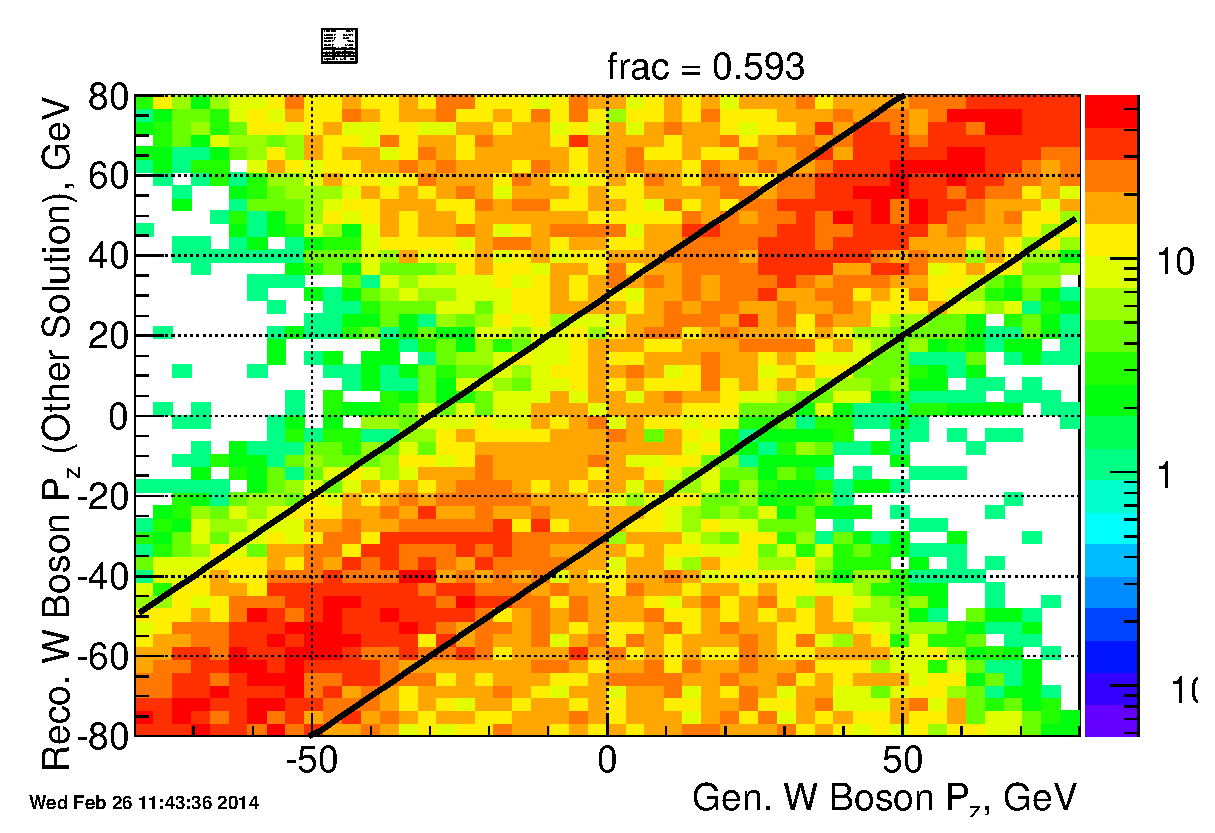
\includegraphics[scale=0.43]{images/P_long_study/hRecoVsWBosonPz_OtherSol}
\end{center}
\caption{MC distribution of reconstructed versus generated $P^{W}_{L}$ for the first solution ({\it left}) and the second solution ({\it right}) respectively.}
\label{fig:plot_hRecoVsWBosonPz} 
\end{figure} 
Thus, we investigated the fraction of well reconstructed events in bins of  generated $P^{W}_{L}$, as shown in Fig.~\ref{fig:plot_hWBosonPz_GoodRecoFraction}.
It is evident that the first solution better reconstructs  $P^{W}_{L}<40$~GeV whereas the second solution works better for larger longitudinal momenta.  
Having in mind that our $W$ bosons are often produced with a longitudinal momentum smaller than 40~GeV, we chose the solution smaller in magnitude, namely the first solution, to reconstruct the boson kinematics because it leads to a much smaller fraction of mis-reconstructed events in our kinematic domain. A data/MC comparison for the $P^{W}_{L}$ after all the reconstruction is done, is shown in Fig.~\ref{fig:plot_DataMc_Wp}($right$). One can see how the momentum of the produced $W$ boson can be fully reconstructed with a satisfactory data/MC agreement. 
 
\begin{figure}[htbp]
\begin{center}
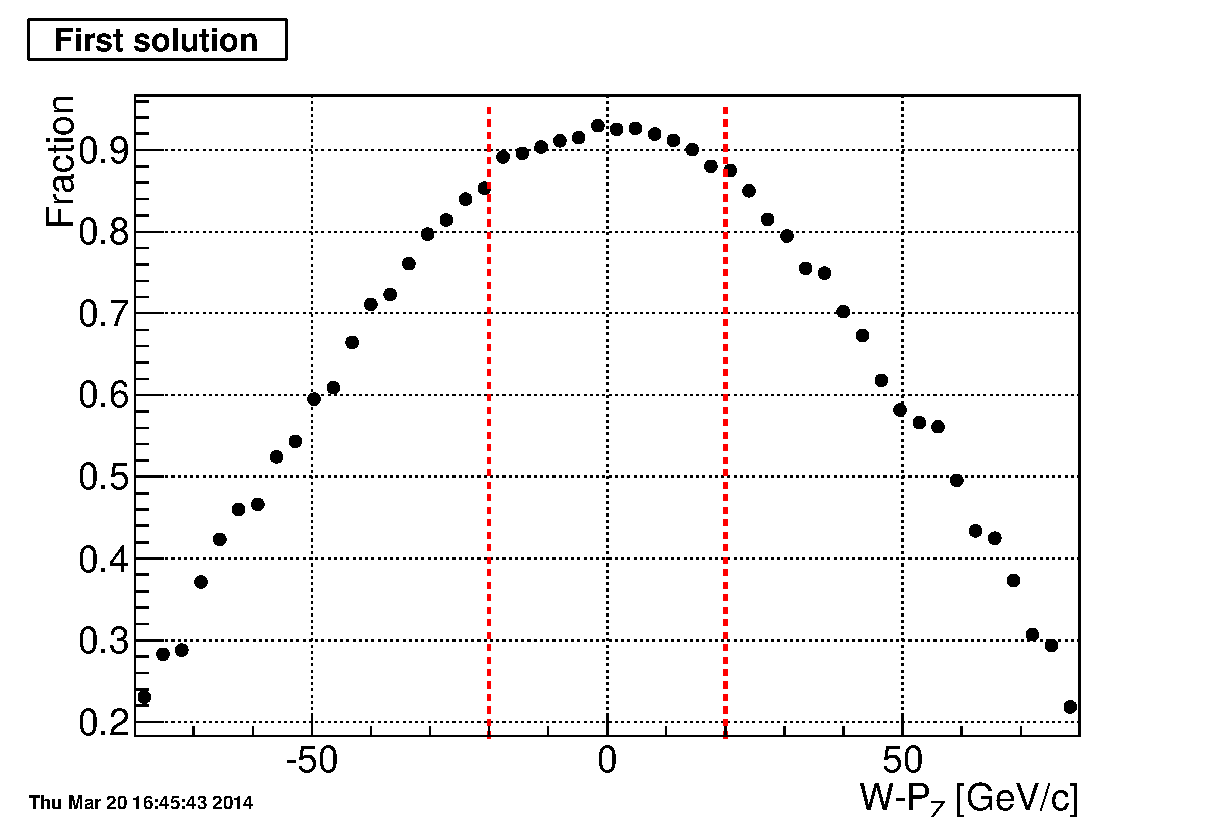
\includegraphics[scale=0.4]{images/P_long_study/hWBosonPz_GoodRecoFraction}
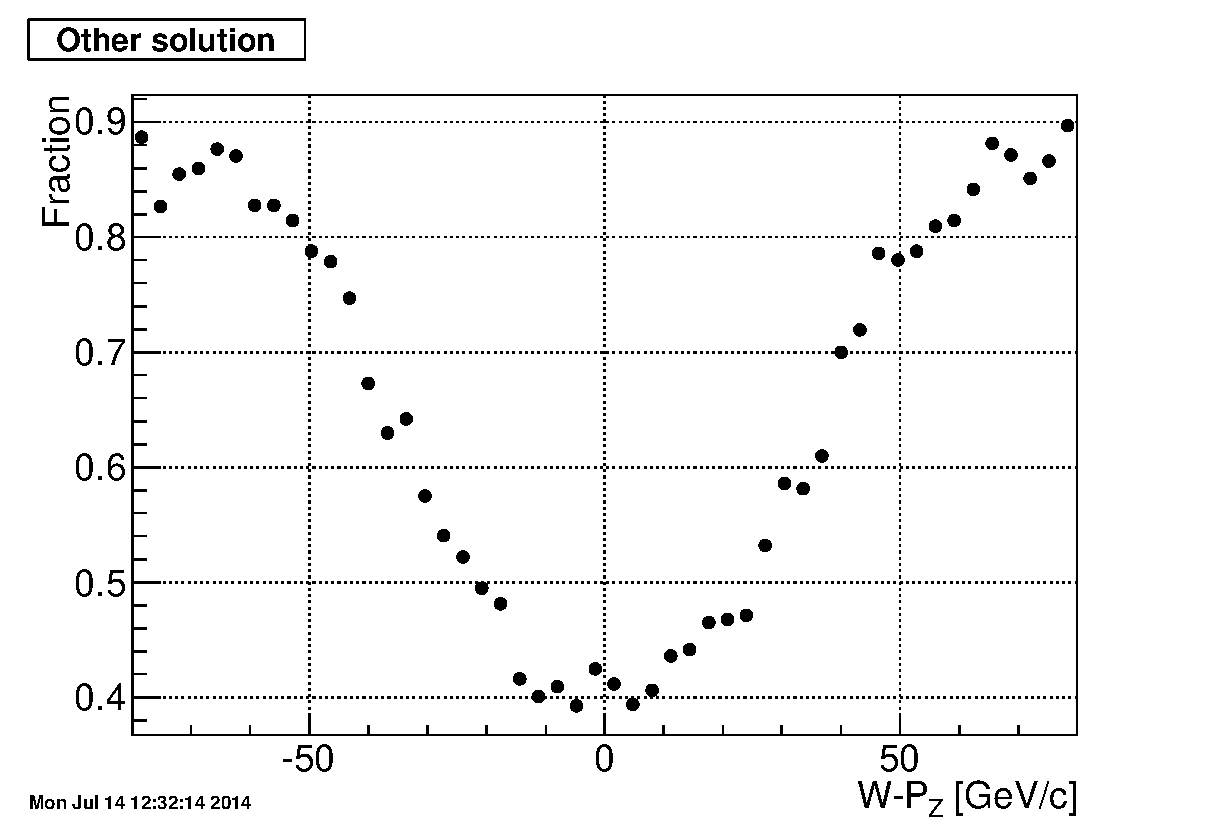
\includegraphics[scale=0.4]{images/P_long_study/hWBosonPz_GoodRecoFraction_OtherSol}
\end{center}
\caption{Estimated fraction of well reconstructed events as a function of generated $P^{W}_{L}$ for the first solution ({\it left}) and the second solution ({\it right}) respectively.}
\label{fig:plot_hWBosonPz_GoodRecoFraction} 
\end{figure}
%Background sources coming from $W^{\pm}\rightarrow \tau^{\pm} \nu_{\tau}$, $Z^{0} \rightarrow e^{+}e^{-}$ and QCD events have been estimated to be contained within maximum a few percent of the selected sample.

\begin{figure}[htbp]
\begin{center}
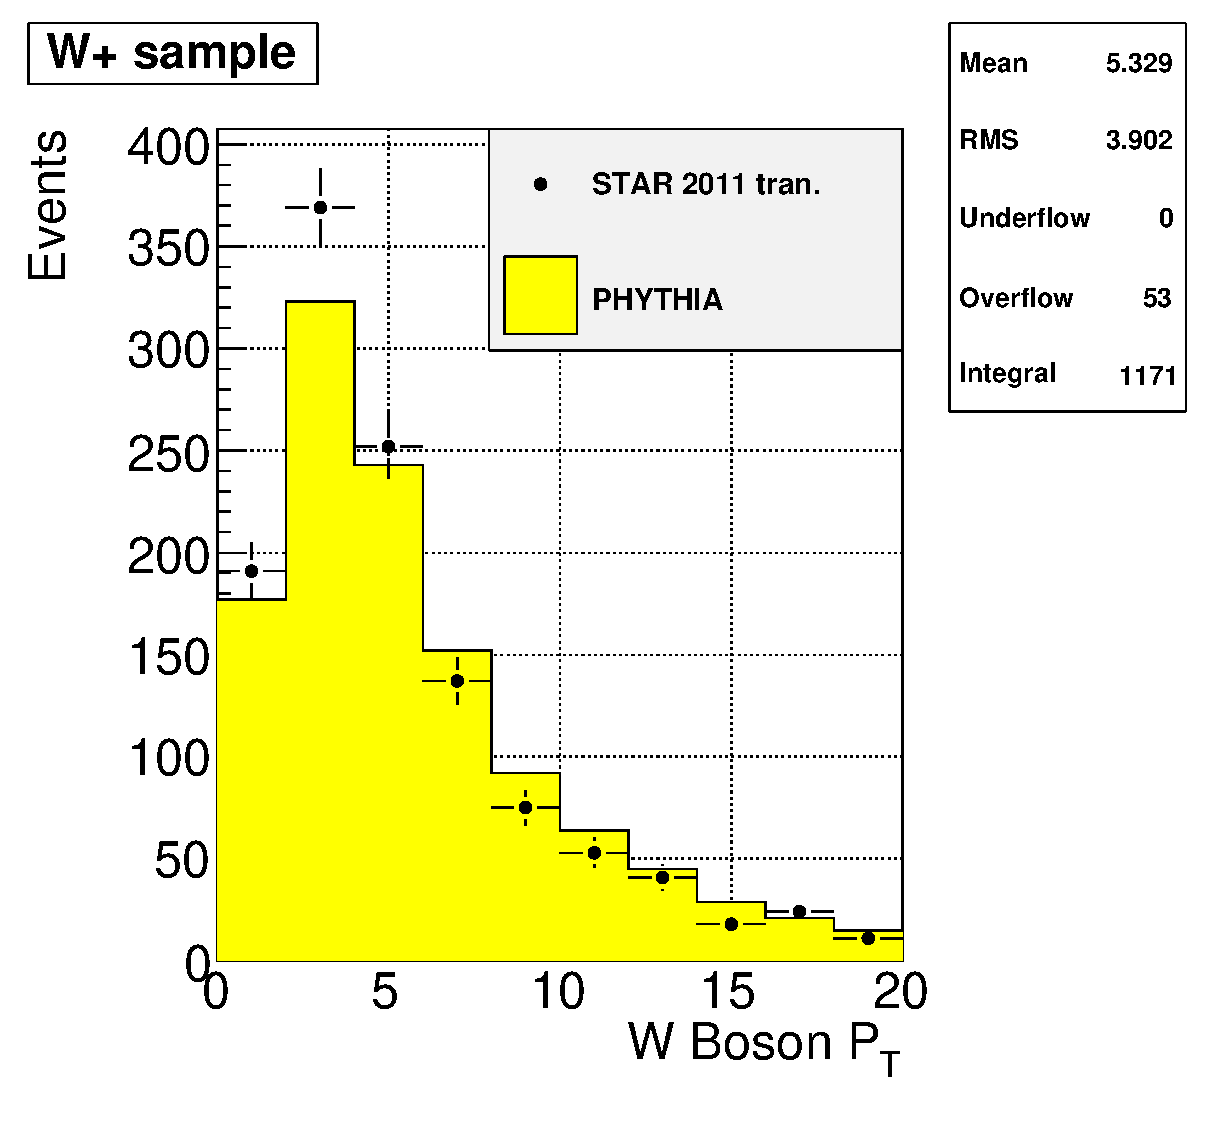
\includegraphics[scale=0.4]{images/DataMC/plot_DataMc_WpPt}
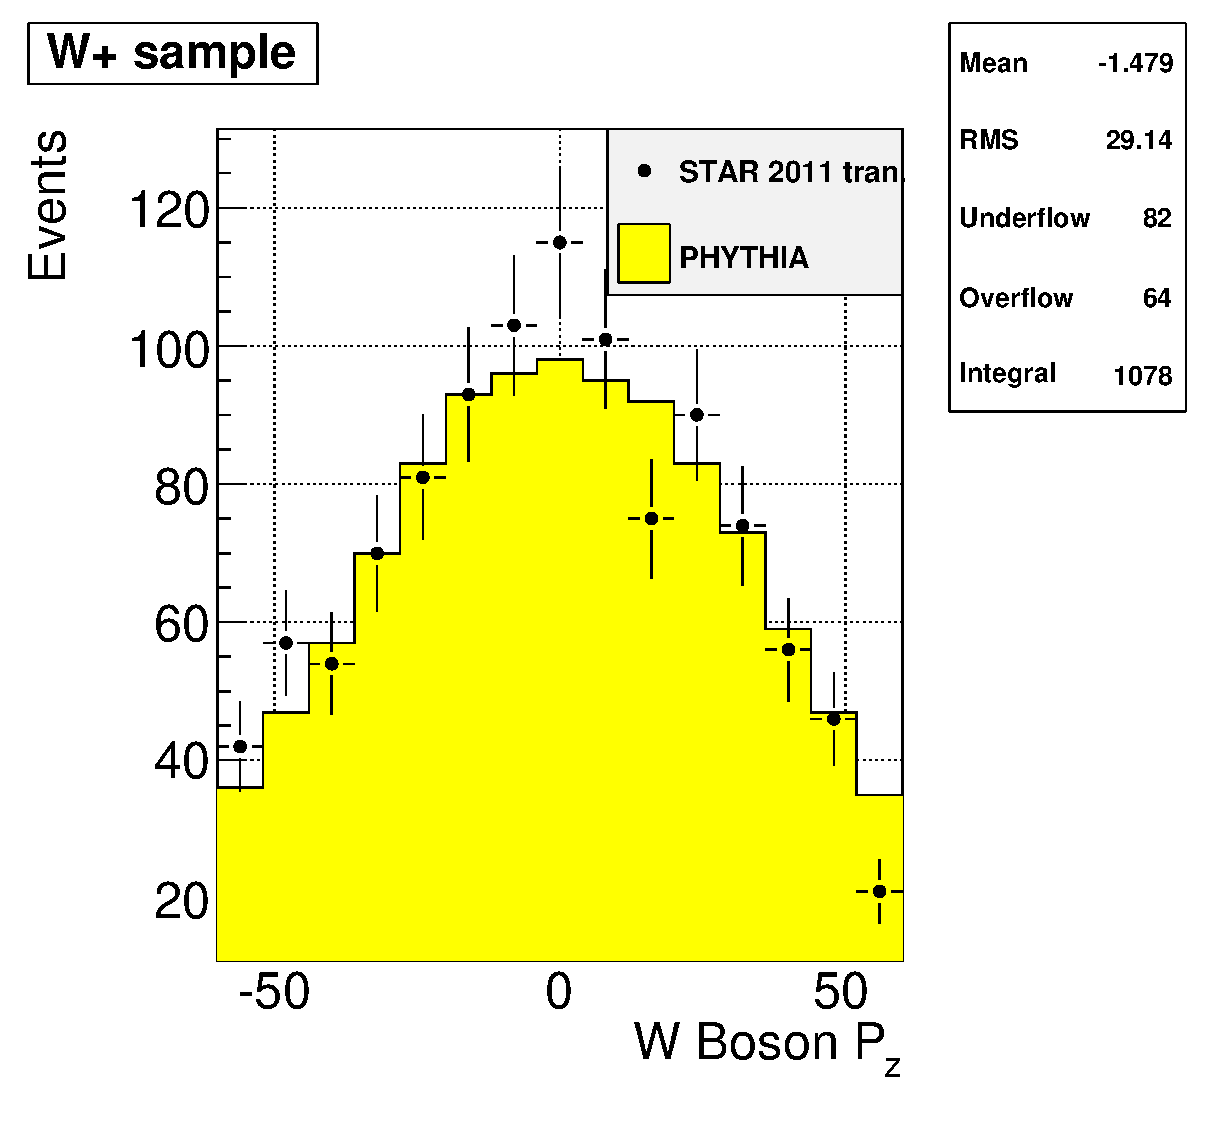
\includegraphics[scale=0.4]{images/DataMC/plot_DataMc_WpPz}
\end{center}
\caption{Data/MC agreement for the W boson $P_{T}$ ($left$) and $P_{L}$ ($right$).}
\label{fig:plot_DataMc_Wp} 
\end{figure}


\subsection{Background estimation}


\begin{figure}[htbp]
\begin{center}
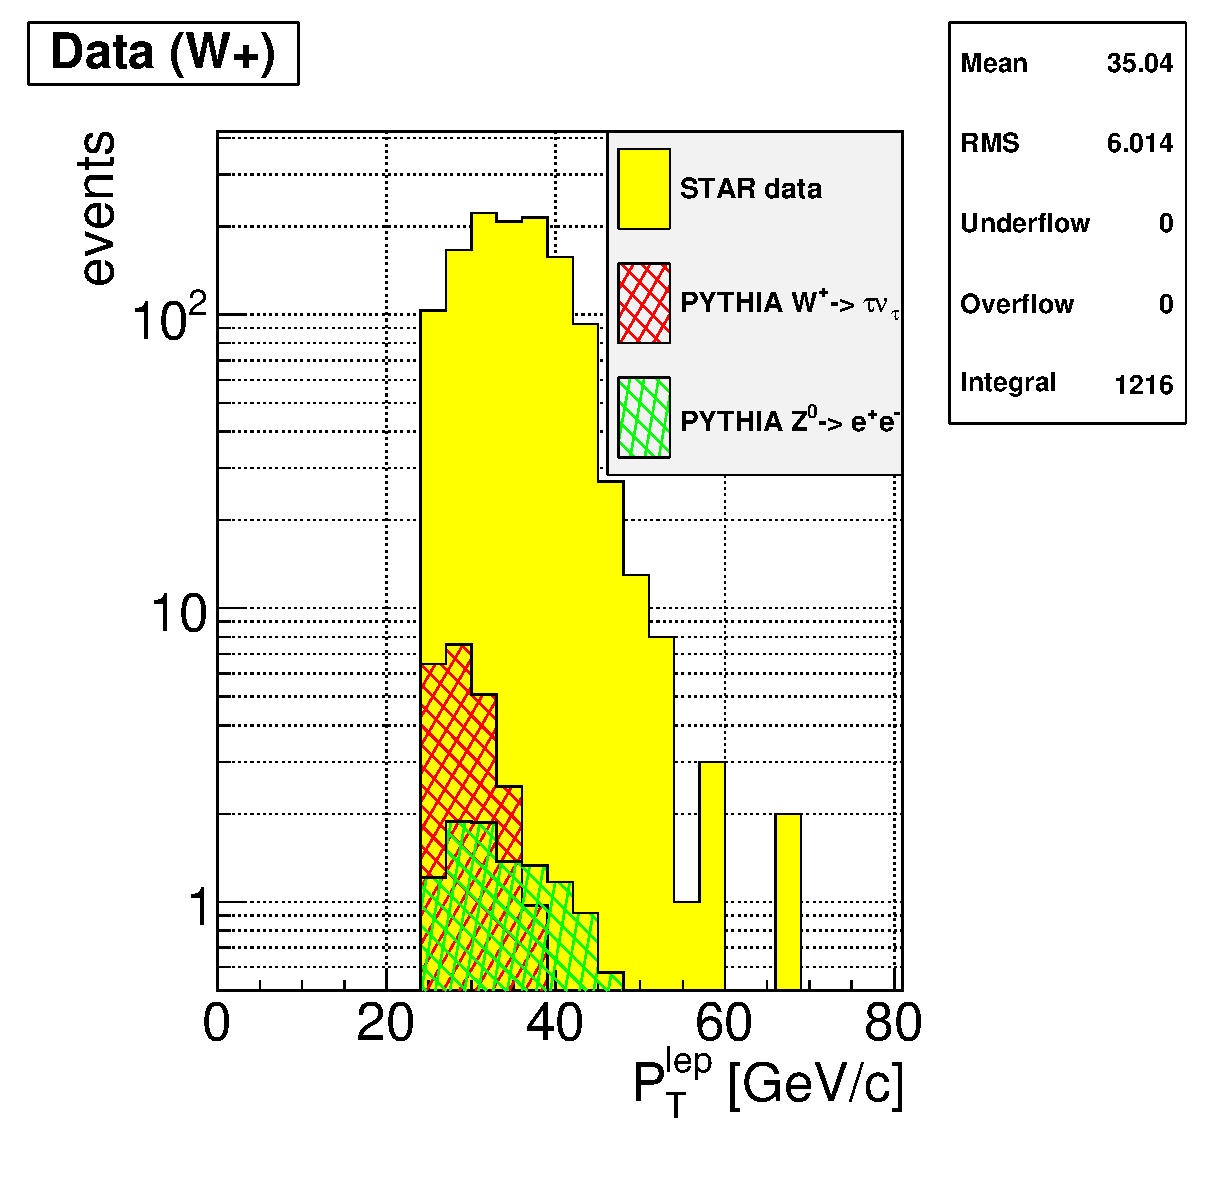
\includegraphics[scale=0.43]{images/backgrounds/plot_4}
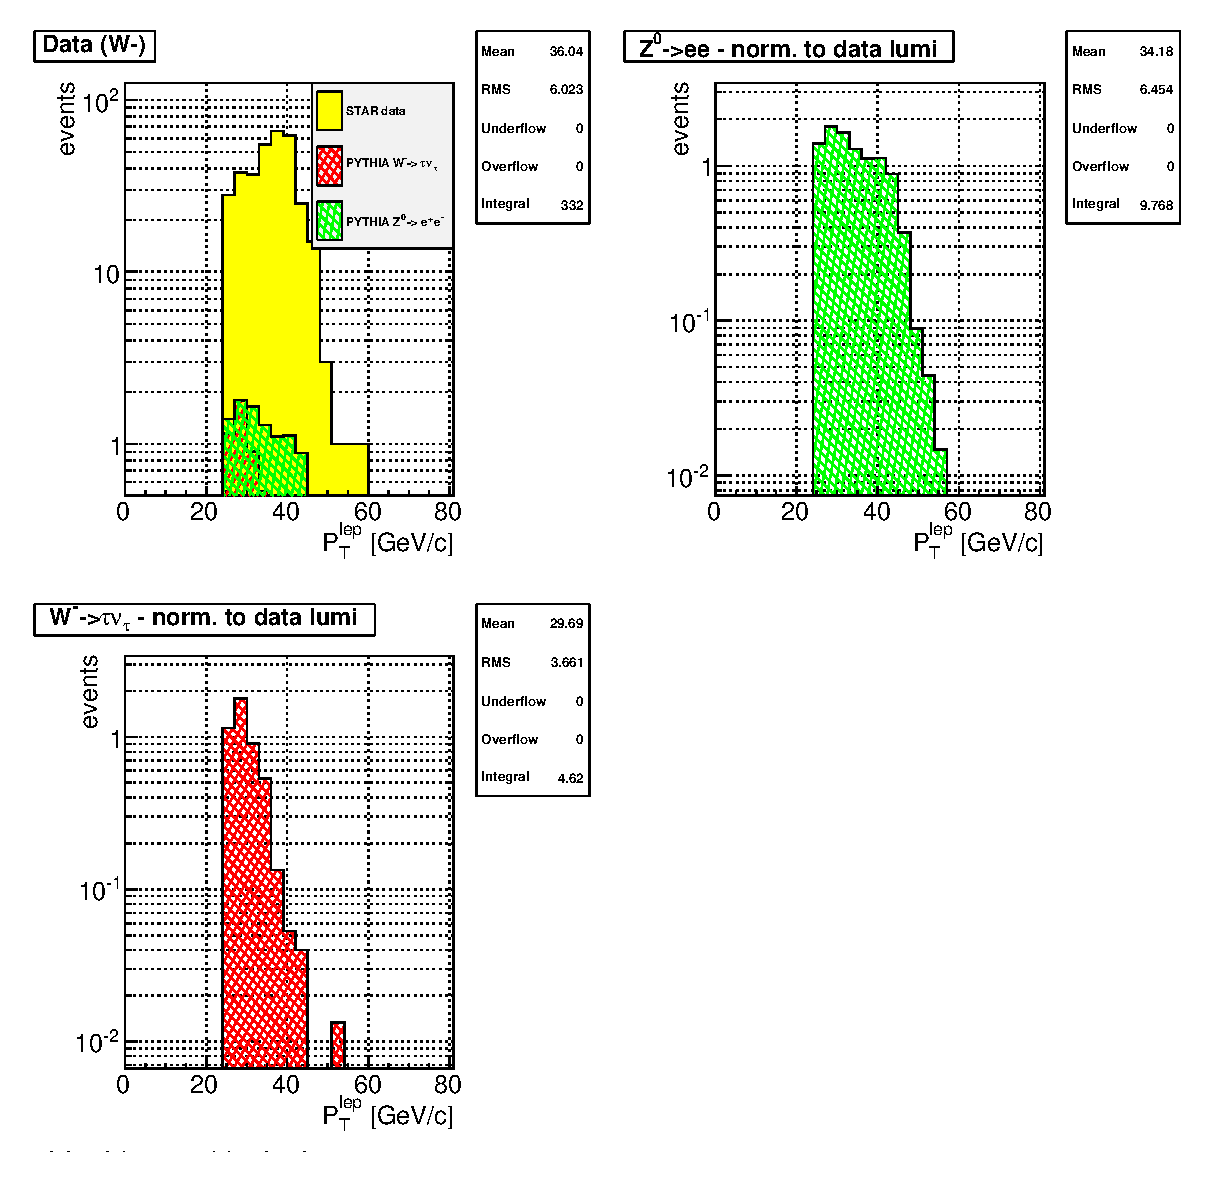
\includegraphics[scale=0.43]{images/backgrounds/plot_6}
\end{center}
\caption{Estimated contribution from the $Z^{0} \rightarrow e^+e^-$ and $W^{\pm} \rightarrow \tau\nu \rightarrow e^+e^-\nu$ backgrounds is shown for the $W^{+}$ ({\it left}) and the $W^{-}$ ({\it right}) data samples respectively.}
\label{fig:plot_WZ_backgrounds} 
\end{figure}


\begin{figure}[htbp]
\begin{center}
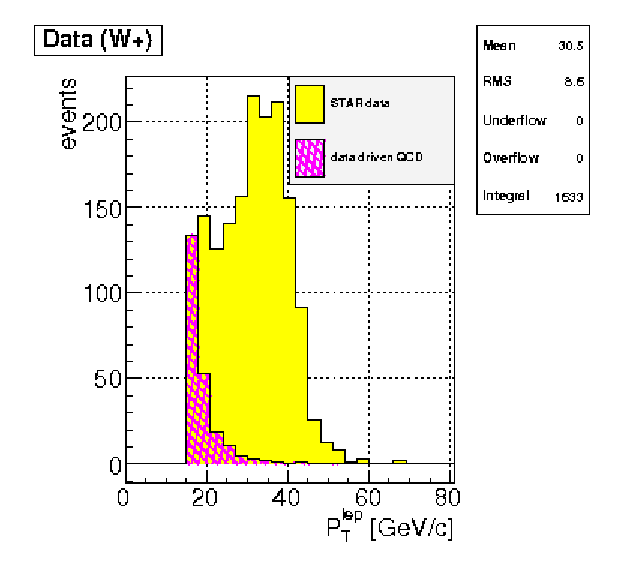
\includegraphics[scale=0.8]{images/backgrounds/plot_4c-1}
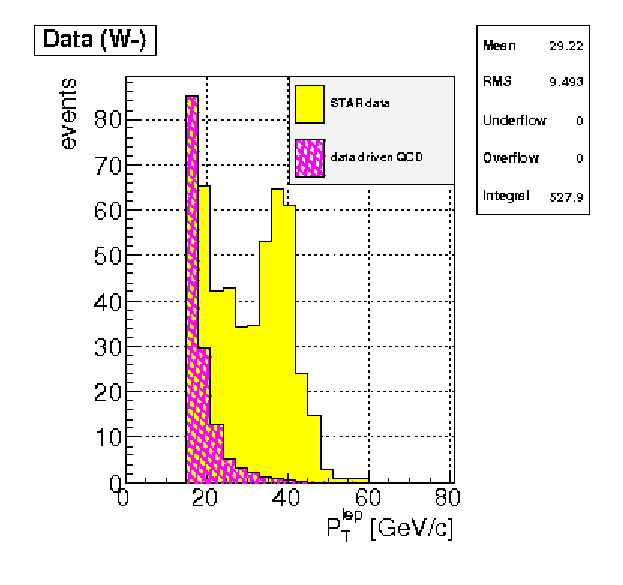
\includegraphics[scale=0.8]{images/backgrounds/plot_6c-1}
\end{center}
\caption{Estimated contribution from the QCD background is shown for the $W^{+}$ ({\it left}) and the $W^{-}$ ({\it right}) data samples respectively. The data-drive QCD sample has been normalized to the lowest lepton-$P_{T}$ bin.}
\label{fig:plot_QCD_bkd_pt15} 
\end{figure}

The background sources considered in this analysis are: 
$Z^{0} \rightarrow e^+e^-$; 
$W^{\pm} \rightarrow \tau\nu \rightarrow e^+e^-\nu$; 
QCD events decaying into leptons, where one of the final leptons is not detected.
The first two sources have been evaluated using MC samples simulated with PYTHIA 6.4 using the ``Perugia tune'' and setting $k_{T}=2$ and $ckin(3)=10$. The MC samples pass trough the GEANT 3 simulation of the STAR detector using the SL11d libraries and are embedded to the run11 p+p transverse zero-bias events. To estimate the contribution from the background, the MC samples have been normalized to the $W^{+}$ and the $W^{-}$ data samples according to the collected luminosity as shown in Fig.~\ref{fig:plot_WZ_backgrounds}. The estimated background-over-signal values for $W^{\pm} \rightarrow \tau\nu$ and $Z^{0} \rightarrow e^+e^-$ are shown in the first columns of Table~\ref{Tab:BoS}. 

\begin{figure}[htbp]
\begin{center}
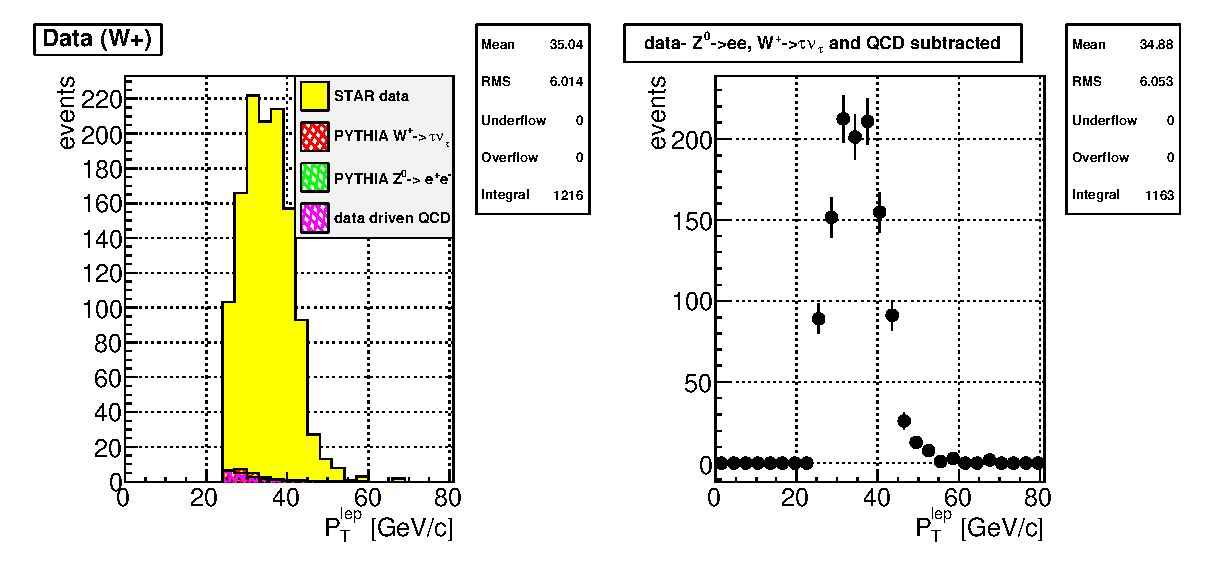
\includegraphics[scale=0.8]{images/backgrounds/plot_5}
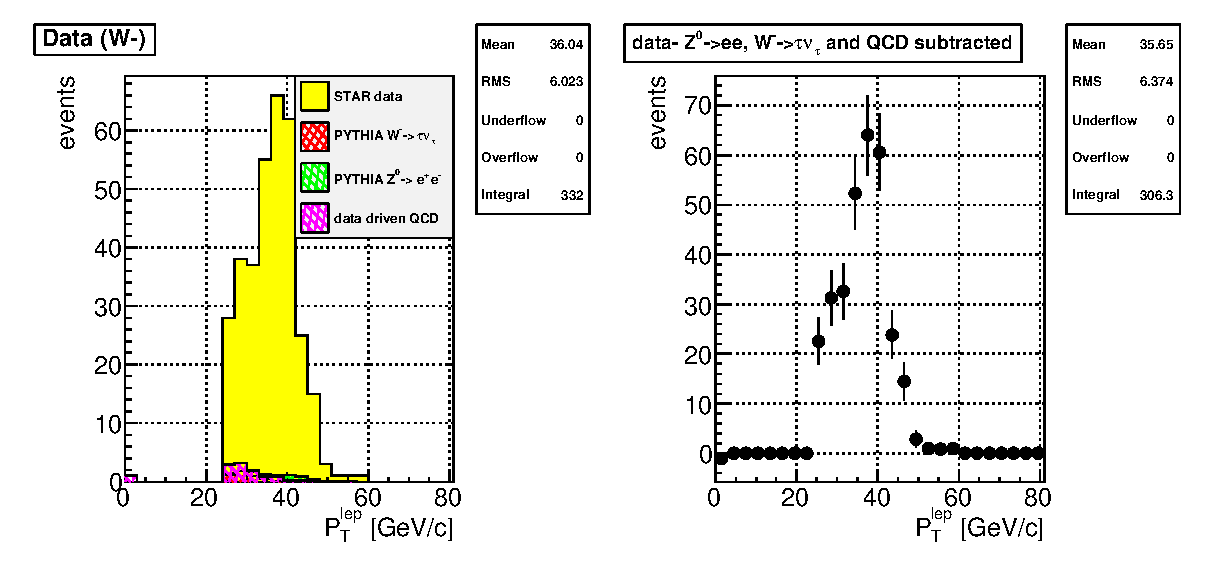
\includegraphics[scale=0.8]{images/backgrounds/plot_7}
\end{center}
\caption{For the $W^{+}$ ({\it upper row}) and the $W^{-}$ ({\it lower row}) data samples, figure shows the estimated contribution from the $Z^{0} \rightarrow e^+e^-$, $W^{\pm} \rightarrow \tau\nu \rightarrow e^+e^-\nu$ and QCD backgrounds ({\it left column}), and the leptonic $P_{T}$ peak after the background sources are statistically subtracted from the data sample ({\it right column}).}
\label{fig:plot_QCD_bkd_pt25} 
\end{figure}

% Table of backgrounds
\begin{table}[htbp]
\centering
\begin{tabular}{| l | c | c  |  c |}
\hline
Process & $W^{\pm}\rightarrow \tau^{\pm} \nu_{\tau}$ & $Z^{0} \rightarrow e^{+}e^{-}$ & QCD \\
\hline
B/S & 1.88\% ($W^{+}$); 1.39\% ($W^{-}$)&  0.88\% ($W^{+}$); 2.94\% ($W^{-}$)& 1.59\% ($W^{+}$); 3.40\% ($W^{-}$)\\
\hline
\end{tabular}
\caption{Background over signal in the $W^{+}$ and $W^{-}$ samples respectively.}
\label{Tab:BoS}
\end{table}

The case of background coming from QCD events is more peculiar since we canon trust the luminosity given by the MC generator. In estimating the background from this source, we followed a ``data-driven'' technique already used at STAR for the $W$ decay analysis with longitudinal beam polarization~\cite{STAR_W_AL_2012-paper, STAR_W_AL_2012-note}. The procedure is the following:

\begin{enumerate}
   \item a QCD dominated data sample was selected reversing the $P_{T}$-balance cut ($P_{T}\text{-balance} < 15$~GeV);
   \item the lepton-$P_{T}$ requirement in our $W$ boson selection (see Sec.~\ref{Wselection}) was lowered to  lepton-$P_{T} > 15$~GeV;
   \item the QCD data sample was normalized to the first lepton-$P_{T}$ bin [15-19~GeV] as shown in Fig.~\ref{fig:plot_QCD_bkd_pt15}, under the assumption that this bin is dominated by QCD events with only a negligible contribution from weak boson production events;
   \item the normalized QCD sample was then compared with out signal sample after the lepton-$P_{T}$ cut has been put back to its original value (lepton-$P_{T} > 25$~GeV), as shown if Fig.~\ref{fig:plot_QCD_bkd_pt25}({\it left column}). 
\end{enumerate}


The estimated fraction of QCD background over signal is shown in Table~\ref{Tab:BoS}({\it last column}) for the $W^{+}$ and $W^{-}$ data sample separately. 

From Tab.~\ref{Tab:BoS} one can see that background sources are under control in the present analysis, the the level of background over signal contained within a few percent. Figure~\ref{fig:plot_QCD_bkd_pt25}({\it right column}) shows how the leptonic $P_{T}$ peak looks like after the background sources are statistically subtracted from the data sample.


\subsection{Systematic uncertainties} \label{Sec:Syst}
The expected systematic uncertainties due to the reconstruction procedure of the boson kinematics have been evaluated via a Monte Carlo challenge. %using a theoretical prediction for the asymmetry from~\cite{Kang:2014}.
Since PYTHIA does not have polarization implemented, we used tables (rapidity and $P_{T}$ bins of W boson) of theoretical predictions for $A_{N}$ with evolution included, confidentially given to us by Z-B Kang and generated from~\cite{Kang:2014}. the procedure is as follows

\begin{itemize}
\item PYTHIA is used to generate samples for $W^{-}$ production (for which $A_{N}$ is predicted to be always positive);
\item each prediction for $A_{N}$ taken from the tables has been assigned to the PYTHIA generated values of W-$y$ and W-$P_{T}$;
\item after the Monte Carlo events are fully reconstructed we look at the distributions of $A_{N}$ in the bins of $y$ and $P_{T}$ we use for the asymmetry measurement of Sec.~\ref{Sec:W-An-measurement};
\item the mean position of the peak in the $A_{N}$ distributions at the generated and reconstructed level, in the same bins of $y$ (Fig.~\ref{fig:SysAnRap}) and $P_{T}$ (Fig.~\ref{fig:SysAnPt}), is compared. In the case of the distributions in bins of rapidity, a gaussian functional form has been fit to better estimate the position of the peak, as shown in Fig.~\ref{fig:SysAnRap}.  
\item We evaluate the relative systematic uncertainty in the corresponding bin as
\begin{align}
Sys(i-bin)=\frac{|mean^{GEN}_{i-bin}-mean^{REC}_{i-bin}|}{mean^{GEN}_{i-bin}}.
\end{align}
\end{itemize}

An additional source of common systematic normalization uncertainty on the single-spin
asymmetries due to the uncertainty in the measured beam polarization has been estimated to be 3.4\%~\cite{RHIC-Pol}.

\begin{figure}[htbp]
\begin{center}
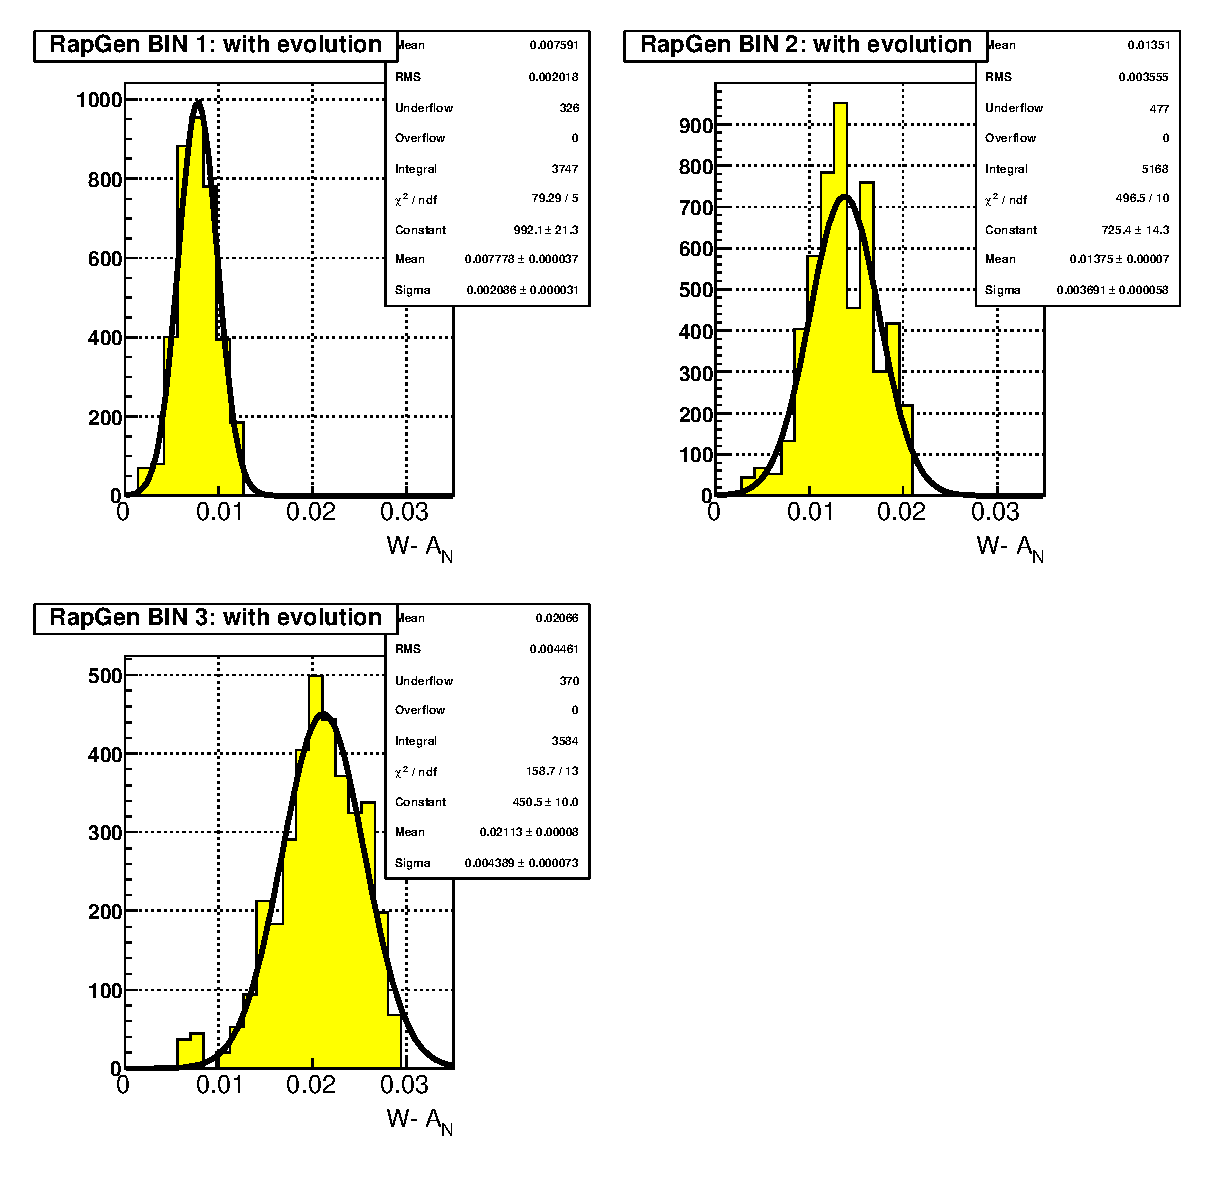
\includegraphics[scale=0.43]{images/systematics/plot_Wm_An_evol_ZK_Vs_RapGen_projs}
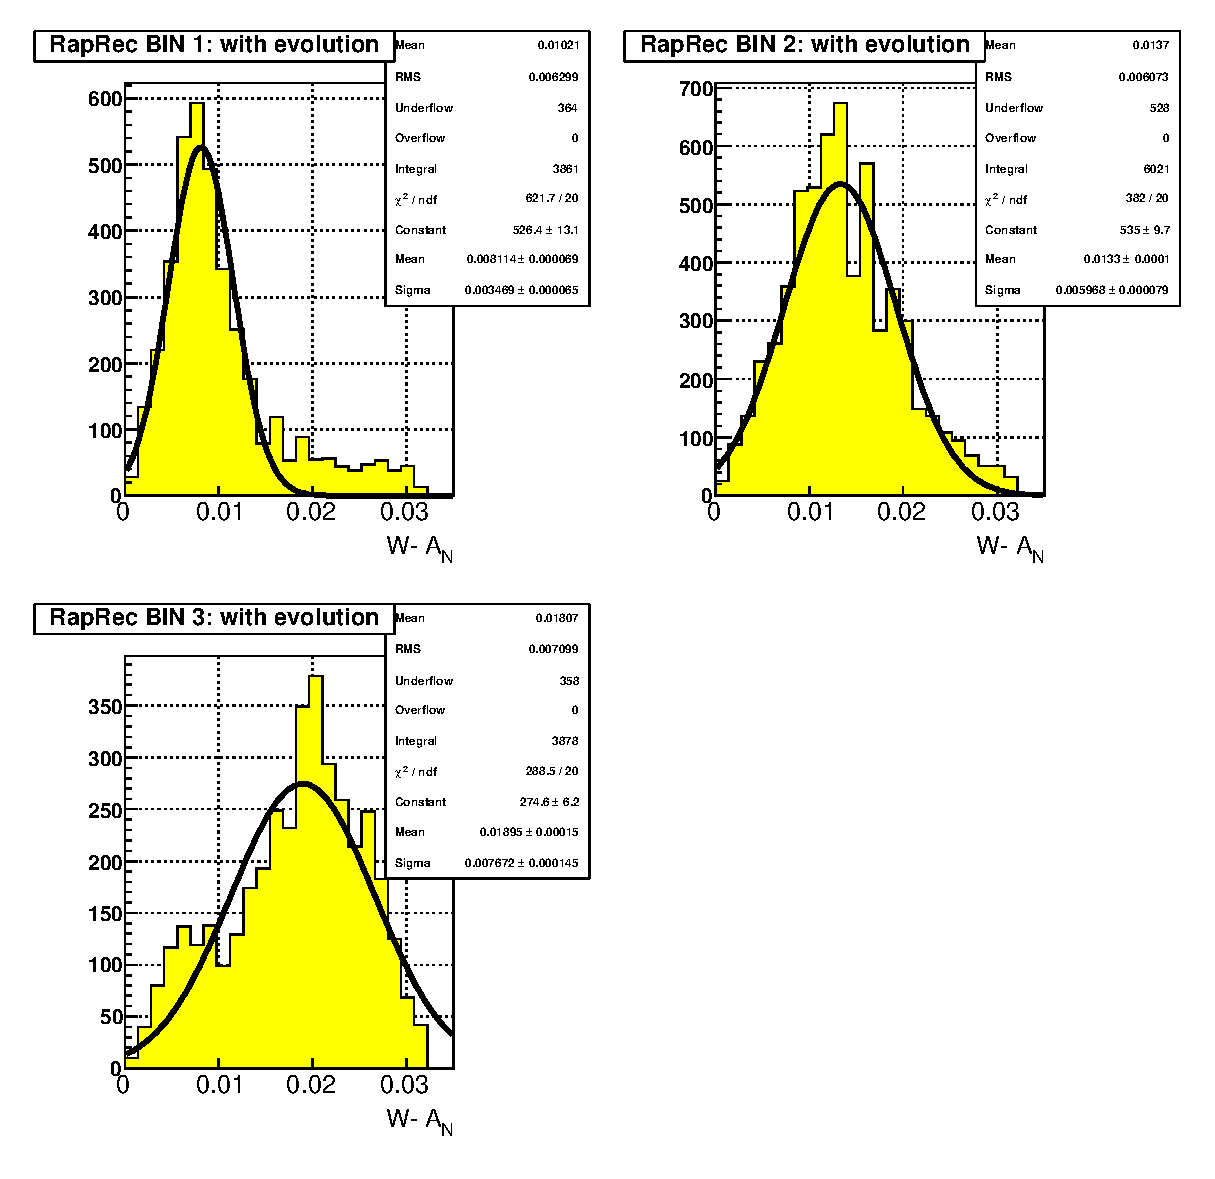
\includegraphics[scale=0.43]{images/systematics/plot_Wm_An_evol_ZK_Vs_RapRec_projs}
\end{center}
\caption{Distribution of $A_{N}$ prediction values at the generated ({\it left}) and reconstructed ({\it right}) level for the three W-rapidity bins used in our asymmetry measurement of Sec.~\ref{Sec:W-An-measurement}.}
\label{fig:SysAnRap} 
\end{figure}

\begin{figure}[htbp]
\begin{center}
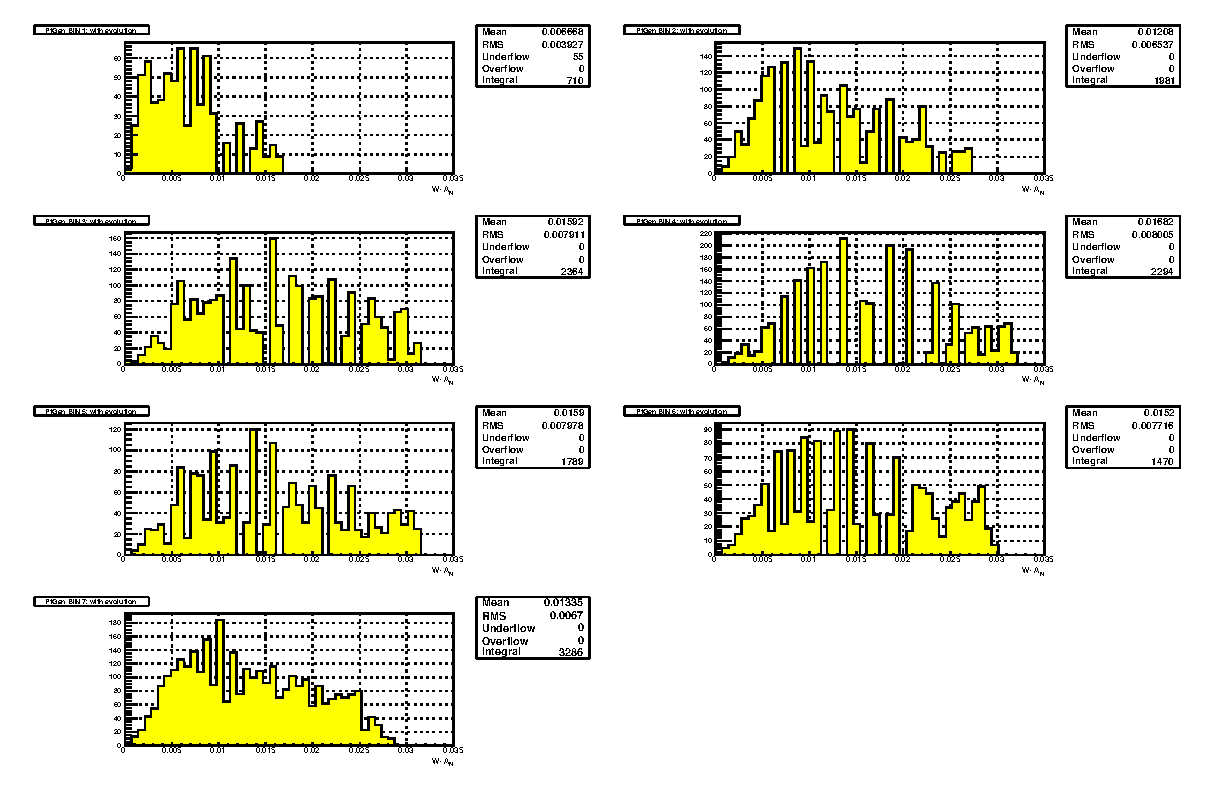
\includegraphics[scale=0.87]{images/systematics/plot_Wm_An_evol_ZK_Vs_PtGen_projs}
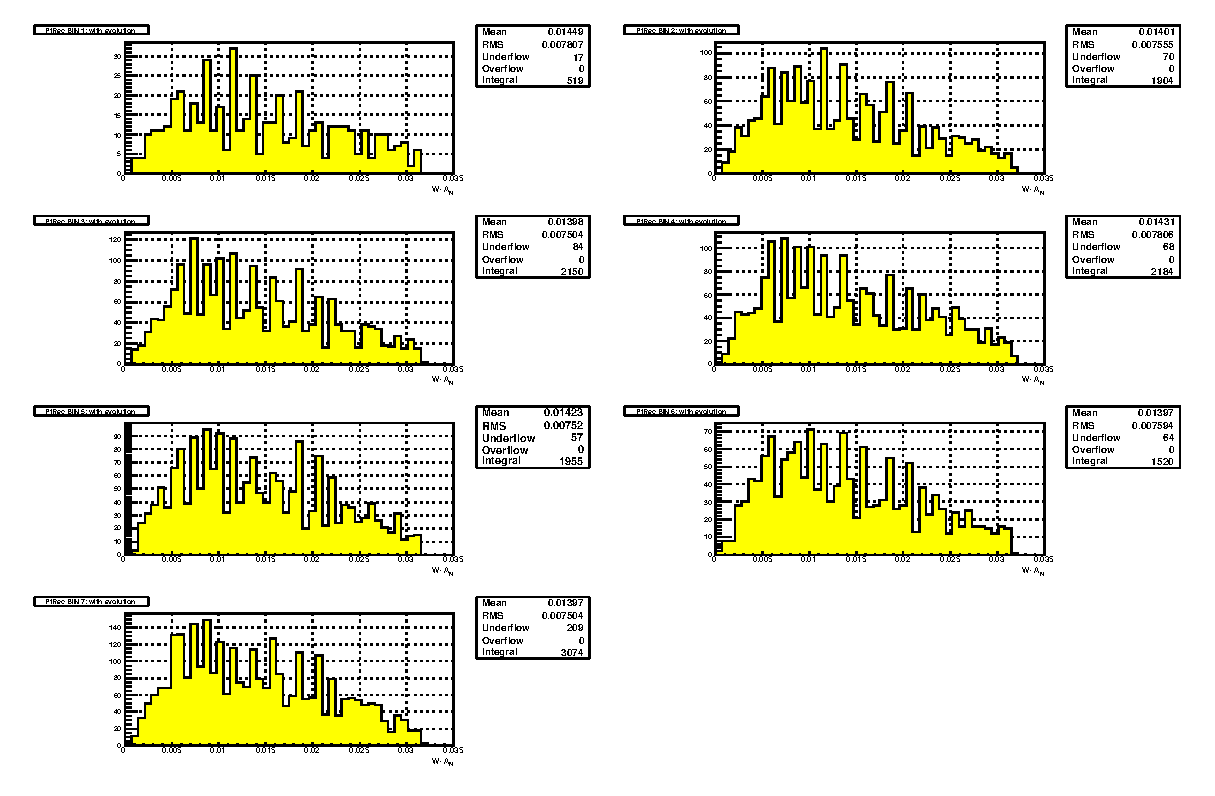
\includegraphics[scale=0.85]{images/systematics/plot_Wm_An_evol_ZK_Vs_PtRec_projs}
\end{center}
\caption{Distribution of $A_{N}$ prediction values at the generated ({\it upper}) and reconstructed ({\it lower}) level for the seven W-$P_{T}$ bins used in our asymmetry measurement of Sec.~\ref{Sec:W-An-measurement}.}
\label{fig:SysAnPt} 
\end{figure}


\section{Asymmetry measurement} \label{Sec:W-An-measurement}
%For the $A_{N}$ measurement we are interested in the interaction
%$p^{\uparrow/\downarrow} p \to W^\pm \to e^\pm \nu_e$ in which the spin direction of one
%of the protons is irrelevant, \textit{i.e} unpolarized protons. 
In measuring $A_{N}$ we assume that the beam polarization vector does not significantly
deviate from the vertical direction given by the normal unit vector $\vec n$
along the vertical $y$ axis, $P \equiv \vec{P} \cdot \vec{n}$. 
We also assume the same magnitude of the polarization vector for
spin-up and spin-down bunches, \textit{i.e.} $P = P_\uparrow = P_\downarrow$.
%For unpolarized cross section $\sigma_0 \equiv (\sigma_\uparrow + \sigma_\downarrow)/2$ 
The single spin asymmetry $A_N$ is expressed as:

\begin{align}
\label{eq_anapower}
A_N &= \frac{\sigma_\uparrow - \sigma_\downarrow}{\sigma_\uparrow +
   \sigma_\downarrow}.
\end{align}

We bin our data sample in three observable variables, $\{y, \phi, P_T\}$, of the produced boson. Thus, 
we calculated $A_{N}$ using the ``left-right'' method~\cite{sqrtFormula}, which helps to cancel out unwanted effects due to geometry and luminosity.

\begin{align}
A_{N } sin(\phi)= \frac{1}{<P>}
\frac{\sqrt{N_\uparrow(\phi_i)N_\downarrow(\phi_i+\pi)} - \sqrt{N_\uparrow(\phi_i+\pi)N_\downarrow(\phi_i)} } 
{\sqrt{N_\uparrow(\phi_i)N_\downarrow(\phi_i+\pi)} + \sqrt{N_\uparrow(\phi_i+\pi)N_\downarrow(\phi_i)}},
\end{align}
where $N$ is the number of recorded events in the $i-th$ bin with a certain spin ($\uparrow \downarrow$) configuration in the ``left'' ($\phi_{i}$) or in the ``right'' ($\phi_{i} + \pi$) side of the detector and $<P>\simeq 53\%$ is the average RHIC beam polarization for 2011 transverse p+p run.  
For the asymmetry measurement the polarization of one of the beams is ignored by combining the
yields with opposite spins, \textit{e.g.}

\begin{align}
N_{\uparrow}   \equiv N_{\uparrow0}   &= N_{\uparrow\uparrow}   + R_{\frac{0\uparrow}{0\downarrow}} N_{\uparrow\downarrow},\\
N_{\downarrow} \equiv N_{\downarrow0} &= N_{\downarrow\uparrow} + R_{\frac{0\uparrow}{0\downarrow}} N_{\downarrow\downarrow},
\end{align}

\noindent
where re-weighting factor $R_{\frac{0\uparrow}{0\downarrow}}$ addresses a
possible relative difference in the spin-up and spin-down intensities of the
other beam. Studies have shown that $R_{\frac{0\uparrow}{0\downarrow}} \approx
1$ with good precision.

%\subsection{preliminary results}
The STAR preliminary results for the $A_{N}$ measurement of the $W^{+}$ and $W^{-}$ boson production are shown separately in Fig.~\ref{Fig:W-An} as a function of $y^{W}$ and $P_{T}^{W}$. 
The systematic uncertainties, evaluated according to the procedure described in Sec.~\ref{Sec:Syst}, are added in quadrature. 
The 3.4\% normalization uncertainty due to the uncertainty in the beam polarization measurement is not shown in the plots. 

\begin{figure}[htbp]
  \centering
  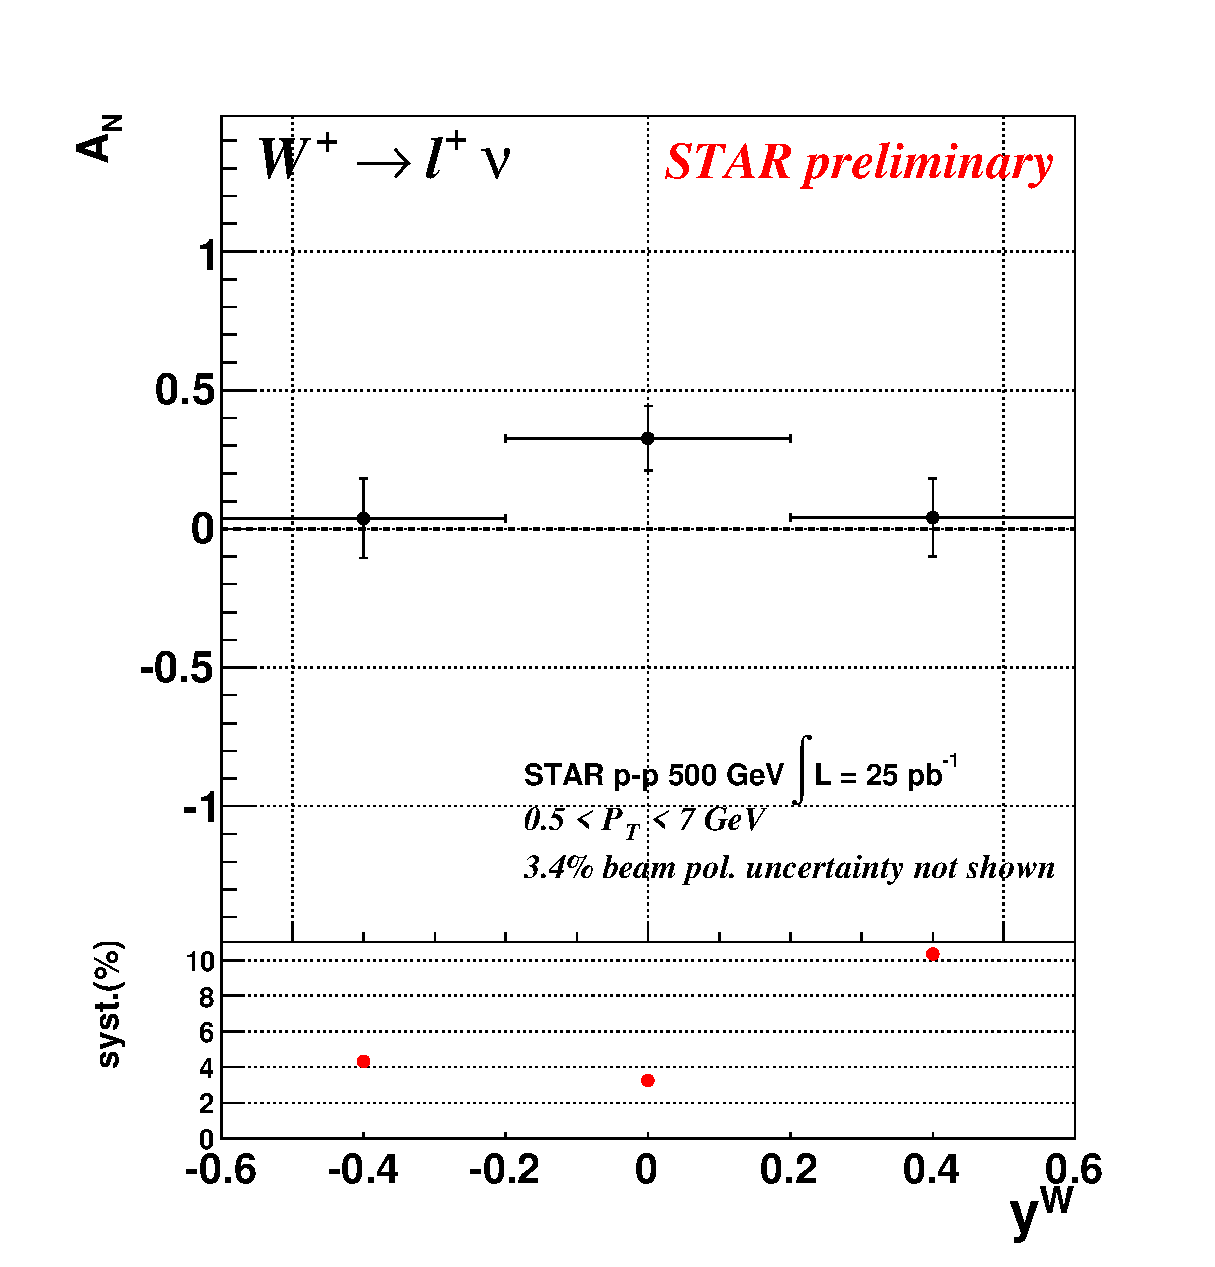
\includegraphics[width=0.49\textwidth]{images/asymmetries/hd_Wp_AsymAmpSqrtVsRap.eps}
  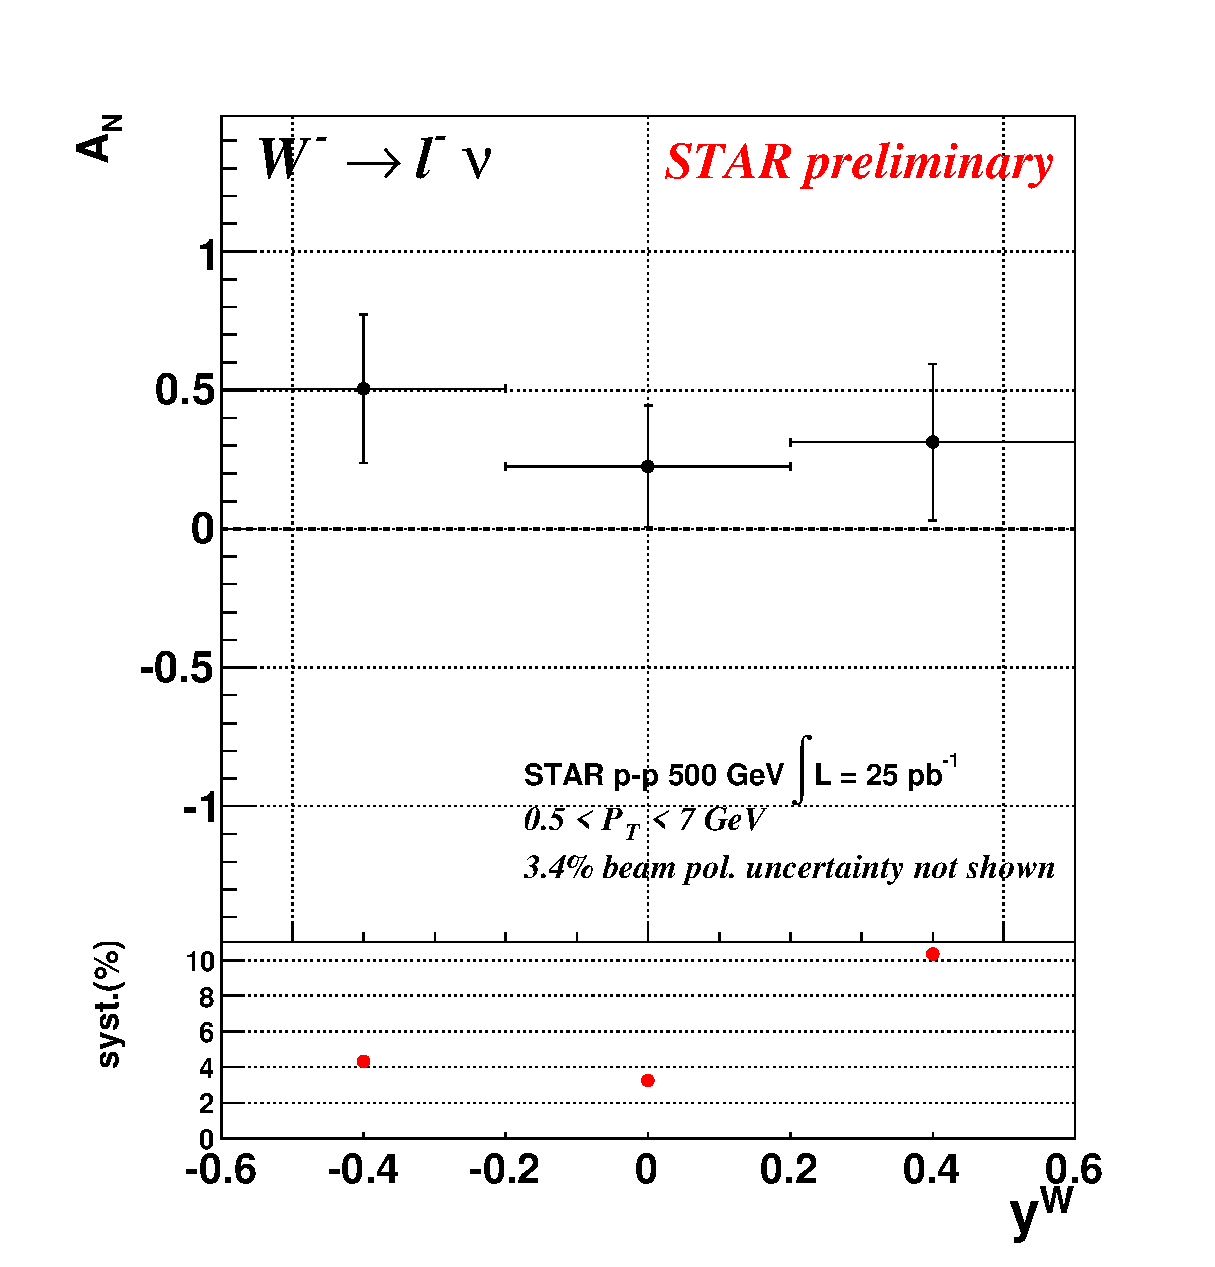
\includegraphics[width=0.49\textwidth]{images/asymmetries/hd_Wm_AsymAmpSqrtVsRap.eps}
  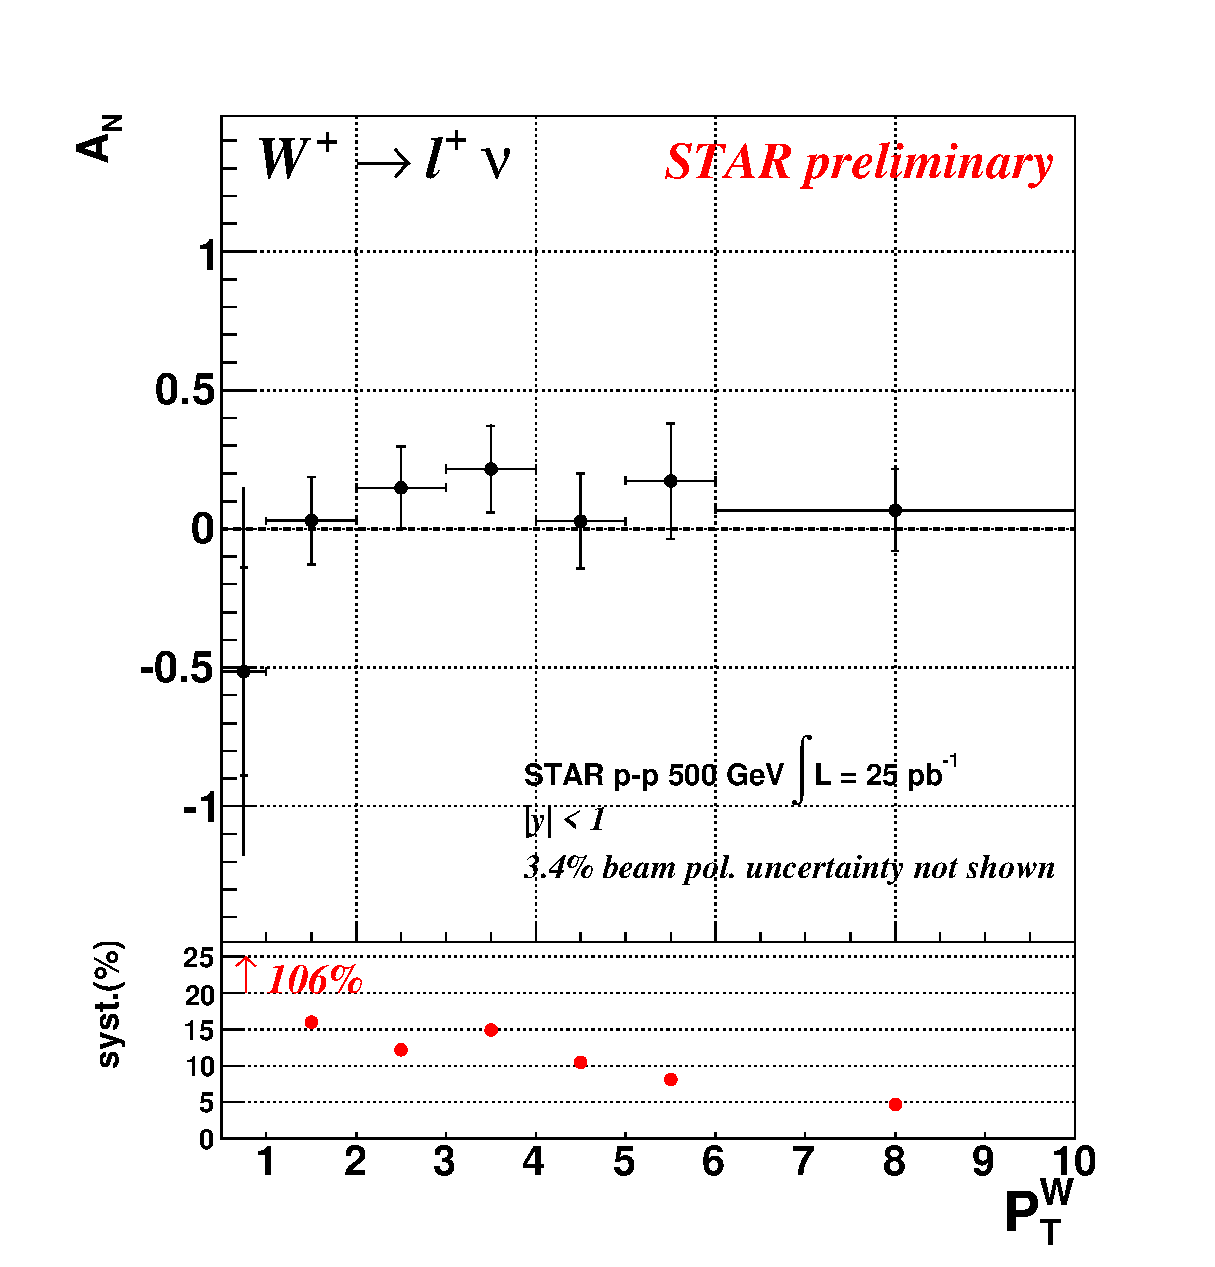
\includegraphics[width=0.49\textwidth]{images/asymmetries/hd_Wp_AsymAmpSqrtVsPt.eps}
  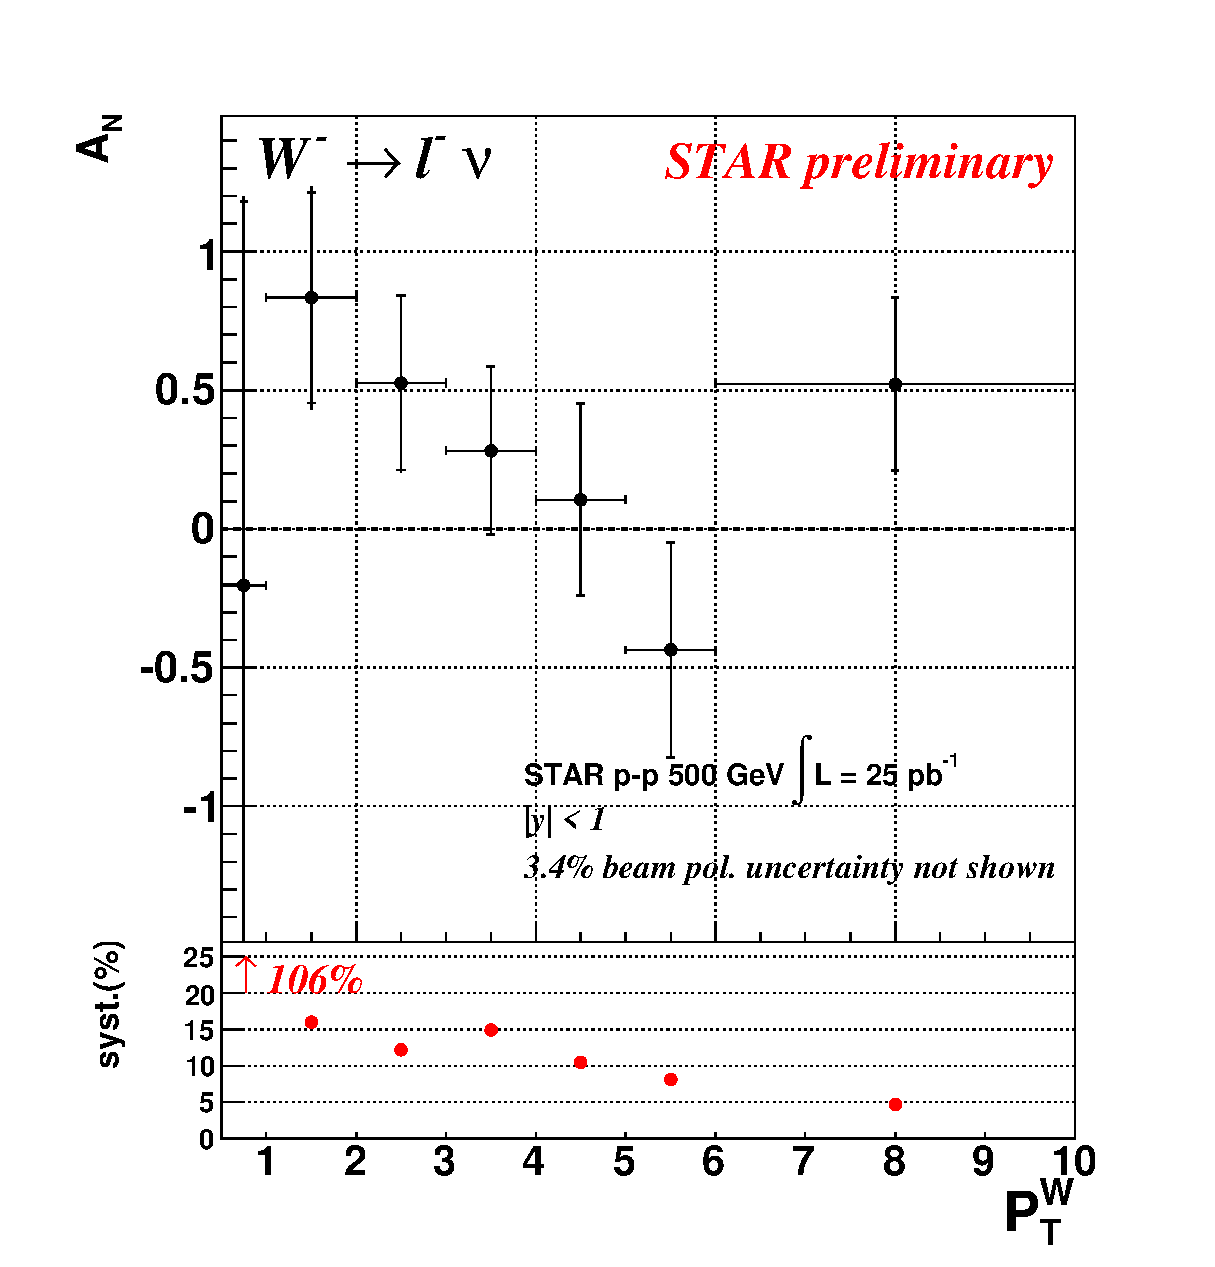
\includegraphics[width=0.49\textwidth]{images/asymmetries/hd_Wm_AsymAmpSqrtVsPt.eps}
  %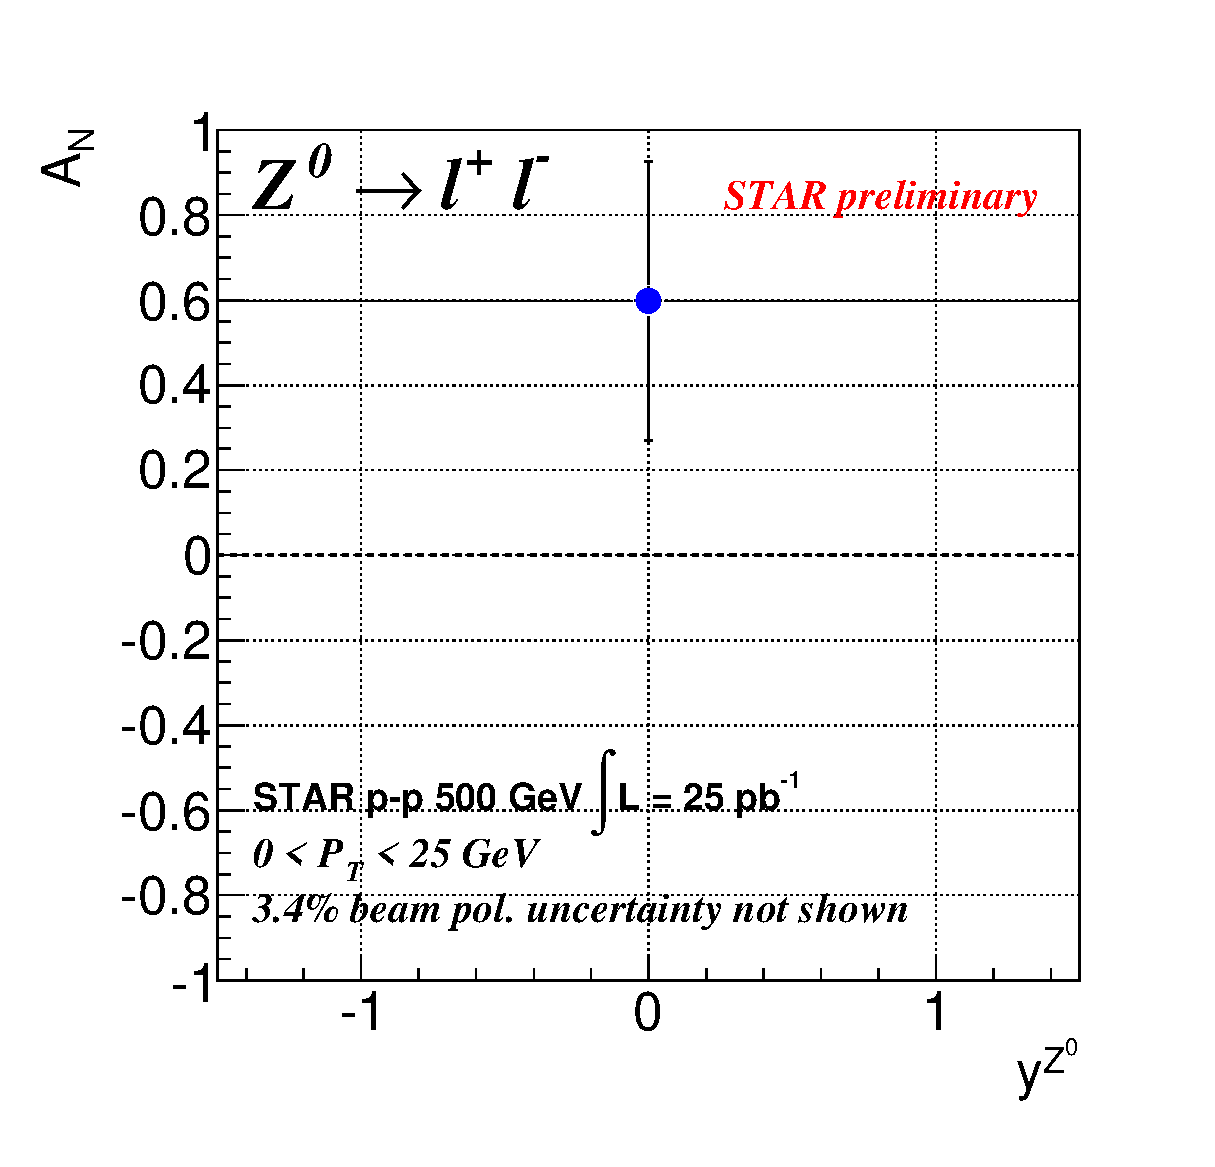
\includegraphics[width=0.44\textwidth]{images/asymmetries/hd_Z0_AsymAmpSqrtVsRap}
  \caption{Transverse single spin asymmetry amplitude for $W^{\pm}$ boson production, the 3.4\% overall systematic uncertainty due to beam polarization is not included.}
  \label{Fig:W-An}
\end{figure}

\section{The $Z^{0}$ selection and asymmetry measurement}
The $Z^{0}\rightarrow e^{+}e^{-}$ process has many advantages: it is experimentally very clean and the boson kinematics are easy to reconstruct since there is no neutrino in the final decay (thus it carries only the overall systematics coming from the polarization measurement), it is background free, the decay electrons peak within the STAR detector acceptance and the asymmetry is expected to be the same size as the $W^{\pm}$ one. The only big disadvantage is the much lower cross section which makes the measurement very statistics hungry. 

A data sample characterized by the $Z^{0}$ signature has been selected 

\begin{itemize}
\item Two high-$P_{T}$ electrons
    \begin{itemize}
    \item lepton-$P_{T}>25$~GeV;
    \item Track-$|\eta|<1$;
    %\item Isolation criterium: $(P^{track}+E^{cluster})/\Sigma[P^{tracks}~\text{in R=0.7 cone]} > 0.8$;
    \item track coming from the maximum ranked vertex;
    \end{itemize}
\item the two electrons must have opposite charge;    
\item $|Z_{vertex}| < 100$~cm; vertex rank $>$ 0;    
\item invariant mass within $\pm 20\%$ from the nominal $Z^{0}$ boson mass.
%\item $0.4 < |\text{Charge(TPC)}*E_{T}\text{(EMC)}/P_{T}\text{(TPC)}| < 1.8$, minimizes charge misidentification.
\end{itemize}

After the whole selection, only 50 events survive. The $Z^{0}$ boson invariant mass, reconstructed using this small event sample, is shown in Fig.~\ref{Fig:Z-M}. The $Z^{0}$ boson kinematics have been reconstructed from the two leptons decay, Fig.~\ref{Fig:Z_kinem} shows the data/MC agreement for the reconstructed $Z^{0}$ transverse momentum and rapidity.

\begin{figure}[htbp]
  \centering
  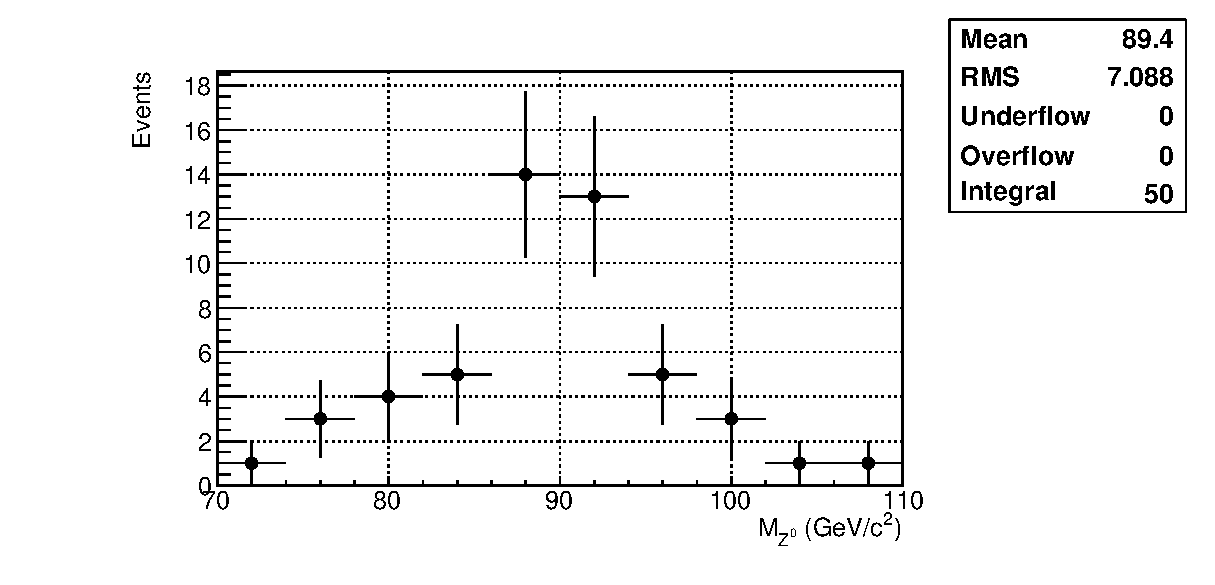
\includegraphics[width=0.85\textwidth]{images/Z_kinematics/Z0_plot_2}
  \caption{Invariant mass of the produced $Z^{0}$ boson.}
  \label{Fig:Z-M}
\end{figure}

\begin{figure}[htbp]
  \centering
  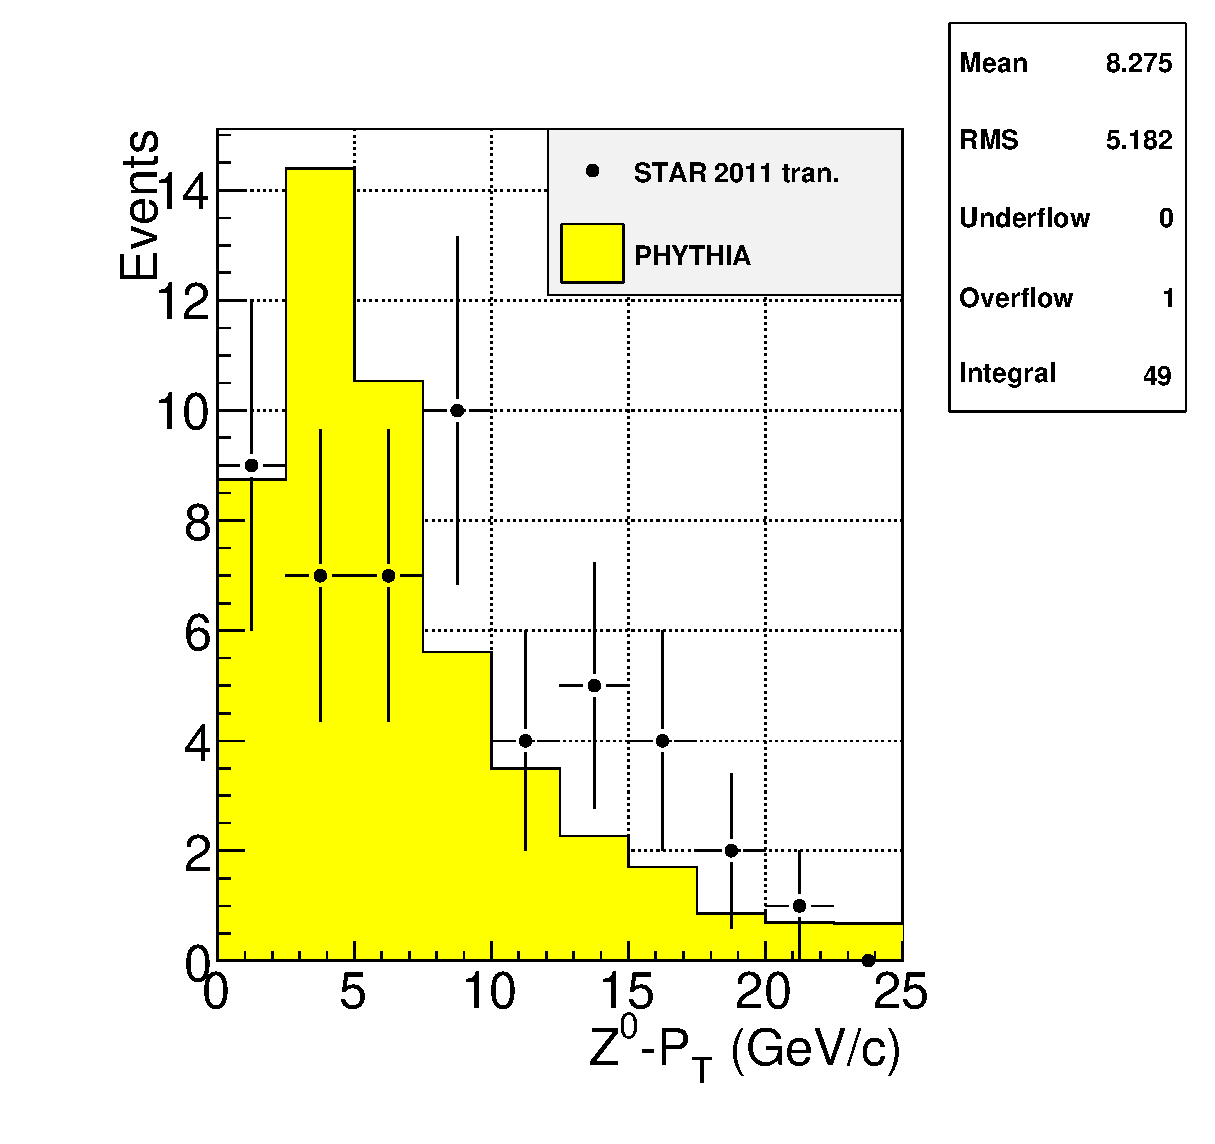
\includegraphics[width=0.45\textwidth]{images/Z_kinematics/plot_DataMc_Z0Pt}
  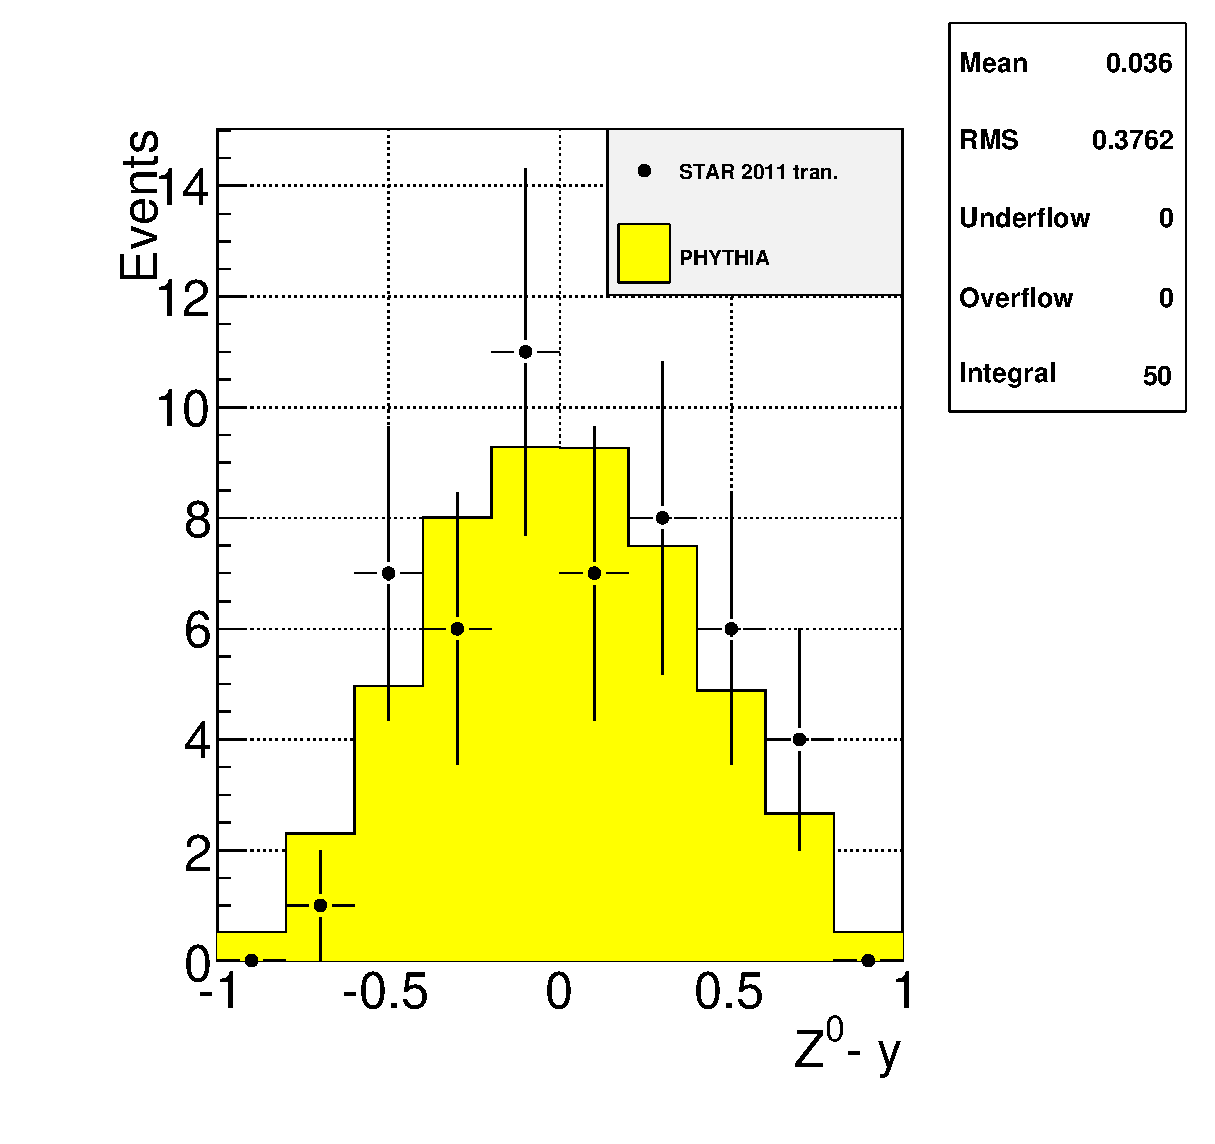
\includegraphics[width=0.45\textwidth]{images/Z_kinematics/plot_DataMc_Z0Rapidity}
  \caption{Data/MC agreement for the reconstructed $P_{T}$ ({\it left}) and rapidity ({\it right}) of the produced $Z^{0}$ boson.}
  \label{Fig:Z_kinem}
\end{figure}

Due to the very small statistics we decided to measure the transverse asymmetry in a single bin for $0 < P_{T} < 20$~GeV and $|y^{Z^{0}}| < 1.5$. 
The STAR preliminary result for the $A_{N}$ measurement of the $Z^{0}$ boson production in a single $y^{Z}$, $P_{T}^{Z}$ bin is shown in Fig.~\ref{Fig:Z-An}. 

\begin{figure}[htbp]
  \centering
  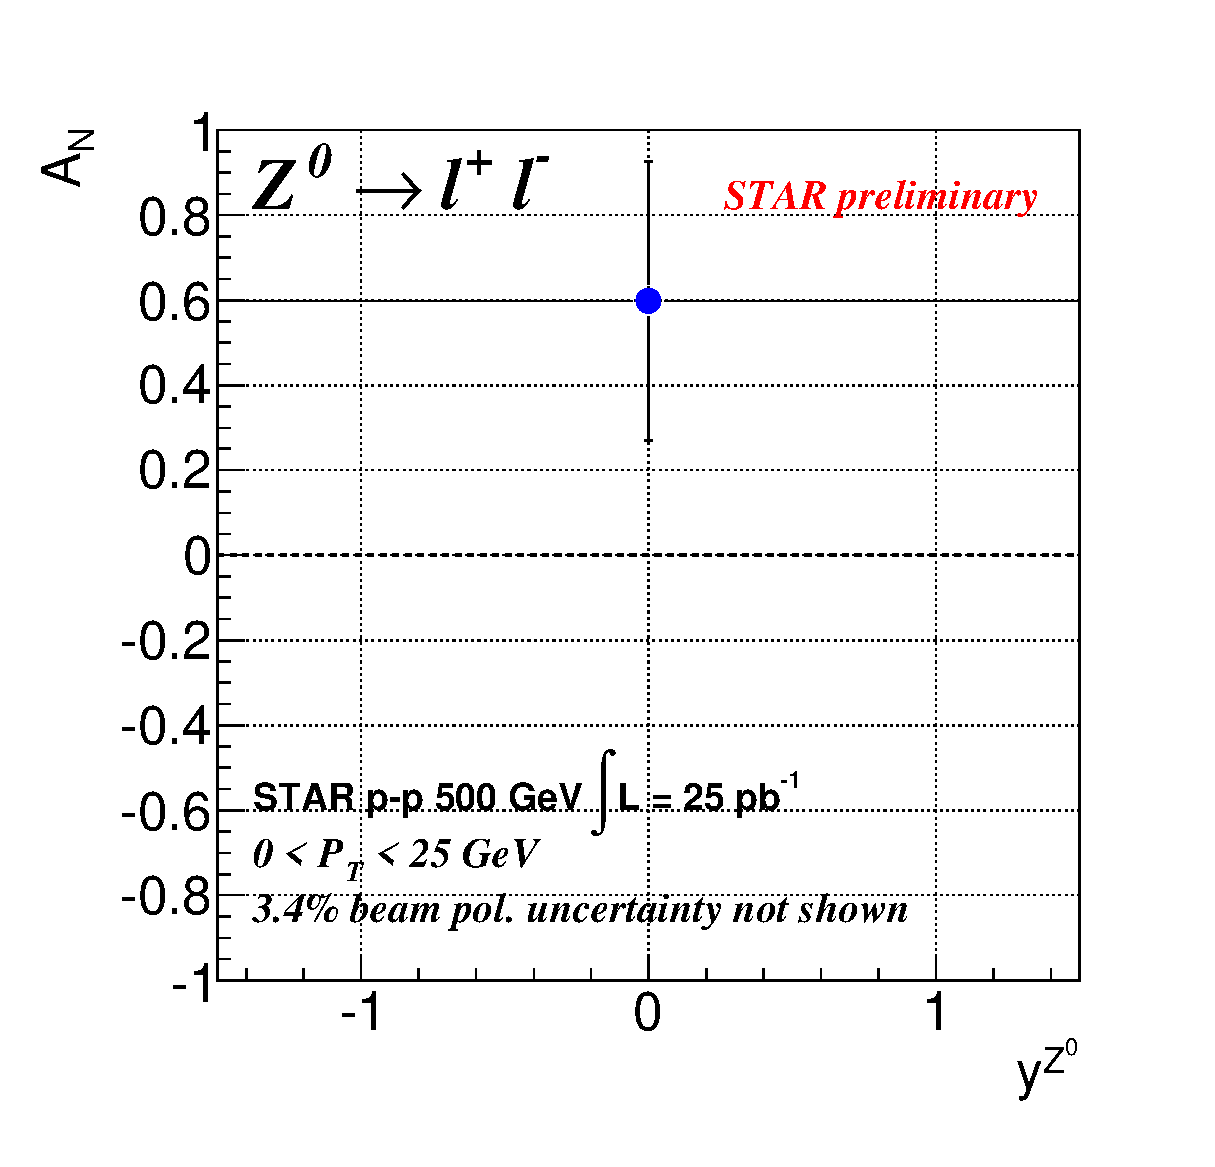
\includegraphics[width=0.6\textwidth]{images/asymmetries/hd_Z0_AsymAmpSqrtVsRap}
  \caption{Transverse single spin asymmetry amplitude for $Z^{0}$ boson production, the 3.4\% overall systematic uncertainty due to beam polarization is not included.}
  \label{Fig:Z-An}
\end{figure}


\section{Conclusions and Outlook}
This preliminary study is a proof-of-principle which shows that STAR is able to measure the transverse single spin asymmetries $A_{N}$ for fully reconstructed $W^{\pm}$, $Z^{0}$ bosons based on a pilot run of transverse polarized p+p collisions at $\sqrt{s}=500$~GeV with a recorded integrated luminosity of $25~\text{pb}^{-1}$. 
The preliminary results from Fig.~\ref{Fig:W-An} can be compared with the most up-to-date theoretical $A_{N}$ predictions for $W^{\pm}$, $Z^{0}$ boson production including TMD-evolution from reference~\cite{Kang:2014}, shown in Fig.~\ref{Fig:An-prediction}, where the error bands have been updated accounting for the current almost complete uncertainty on see-quark functions in the fits~\cite{Kang:private}.
Measuring the production of $W^{\pm}$ bosons at $\sqrt{s}=500$~GeV can lead to the first experimental test of the sign change of the Sivers function. Furthermore, it provides an ideal tool to study the spin-flavor structure of sea quarks inside the proton. The left-handed $W$ boson only couples to (anti)quarks of a certain helicity, giving rise to large parity-violating single spin asymmetries. In addition, the coupling of the $W$ to the weak charge correlates directly to quark flavor. Ignoring quark mixing, $W^{\pm}$ bosons are produced through $u+\bar d (d + \bar u)$ interactions. A measurement of the transverse single spin asymmetry will provide the worldwide first constraint on the sea quark Sivers function in an x-range, where the measured asymmetry in the  $\bar u$ and $\bar d$ unpolarized sea quark distribution functions, as measured by E866~\cite{E866}, can only be explained by strong non-pQCD contributions. Figure~\ref{Fig:Run16Proj} shows the projected uncertainties for transverse single spin asymmetries of $W^{\pm}$, $Z^{0}$ bosons as functions of rapidity and $P_{T}$ for a delivered integrated luminosity of 900 $\text{pb}^{-1}$ compared to 400 $\text{pb}^{-1}$ , at an average beam polarization of $\sim55\%$. RHIC is capable of delivering 900 $\text{pb}^{-1}$ in 14 weeks running using a dynamic $\beta$* squeeze~\cite{beta_squeeze} through the fill. The dynamic $\beta$* squeeze provides a factor 2 increase of the luminosity in a fill as the luminosity profile through the fill is kept flat.

STAR is the only experiment capable of measuring $A_{N}$ for direct photons, for $W^{\pm}$ and $Z^{0}$ bosons, and possibly for DY. It can provide a world-wide unique opportunity to simultaneously test TMD evolution, access the Sivers function for sea quarks, and test the predicted sign-change for the Sivers function.

\begin{figure}[htbp]
  \centering
  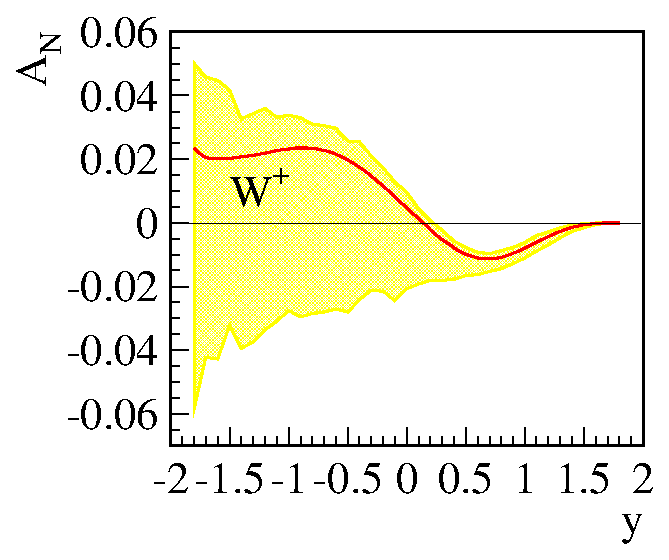
\includegraphics[width=0.32\textwidth]{images/predictions/w_plus.eps}
  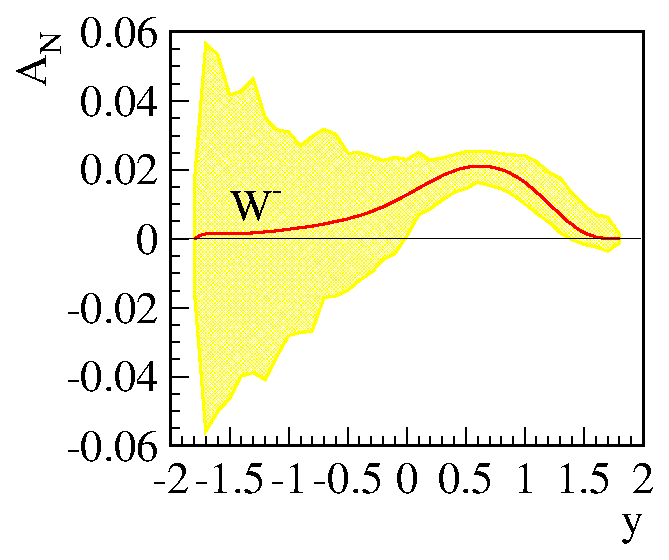
\includegraphics[width=0.32\textwidth]{images/predictions/w_minus.eps}
  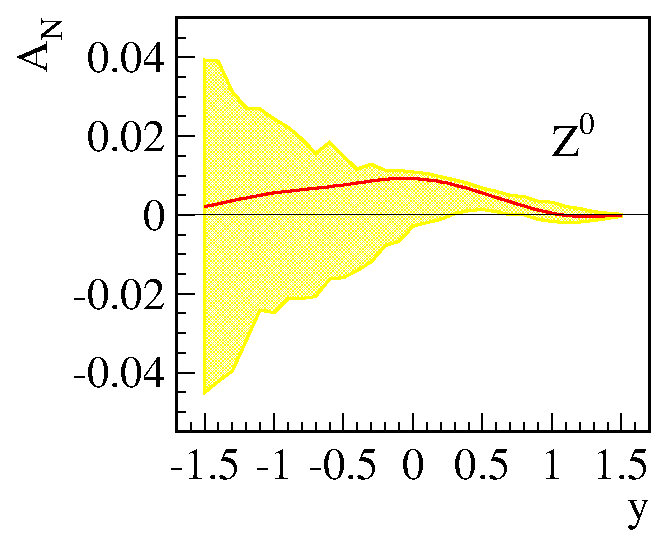
\includegraphics[width=0.32\textwidth]{images/predictions/z0.eps}
  \caption{Theoretical prediction of $A_{N}$ for $W^{\pm}$ and $Z^{0}$ boson production in p+p collisions at $\sqrt{s}=500$~GeV including TMD-evolution~\cite{Kang:2014}.}
  \label{Fig:An-prediction}
\end{figure}

\begin{figure}[htbp]
  \centering
  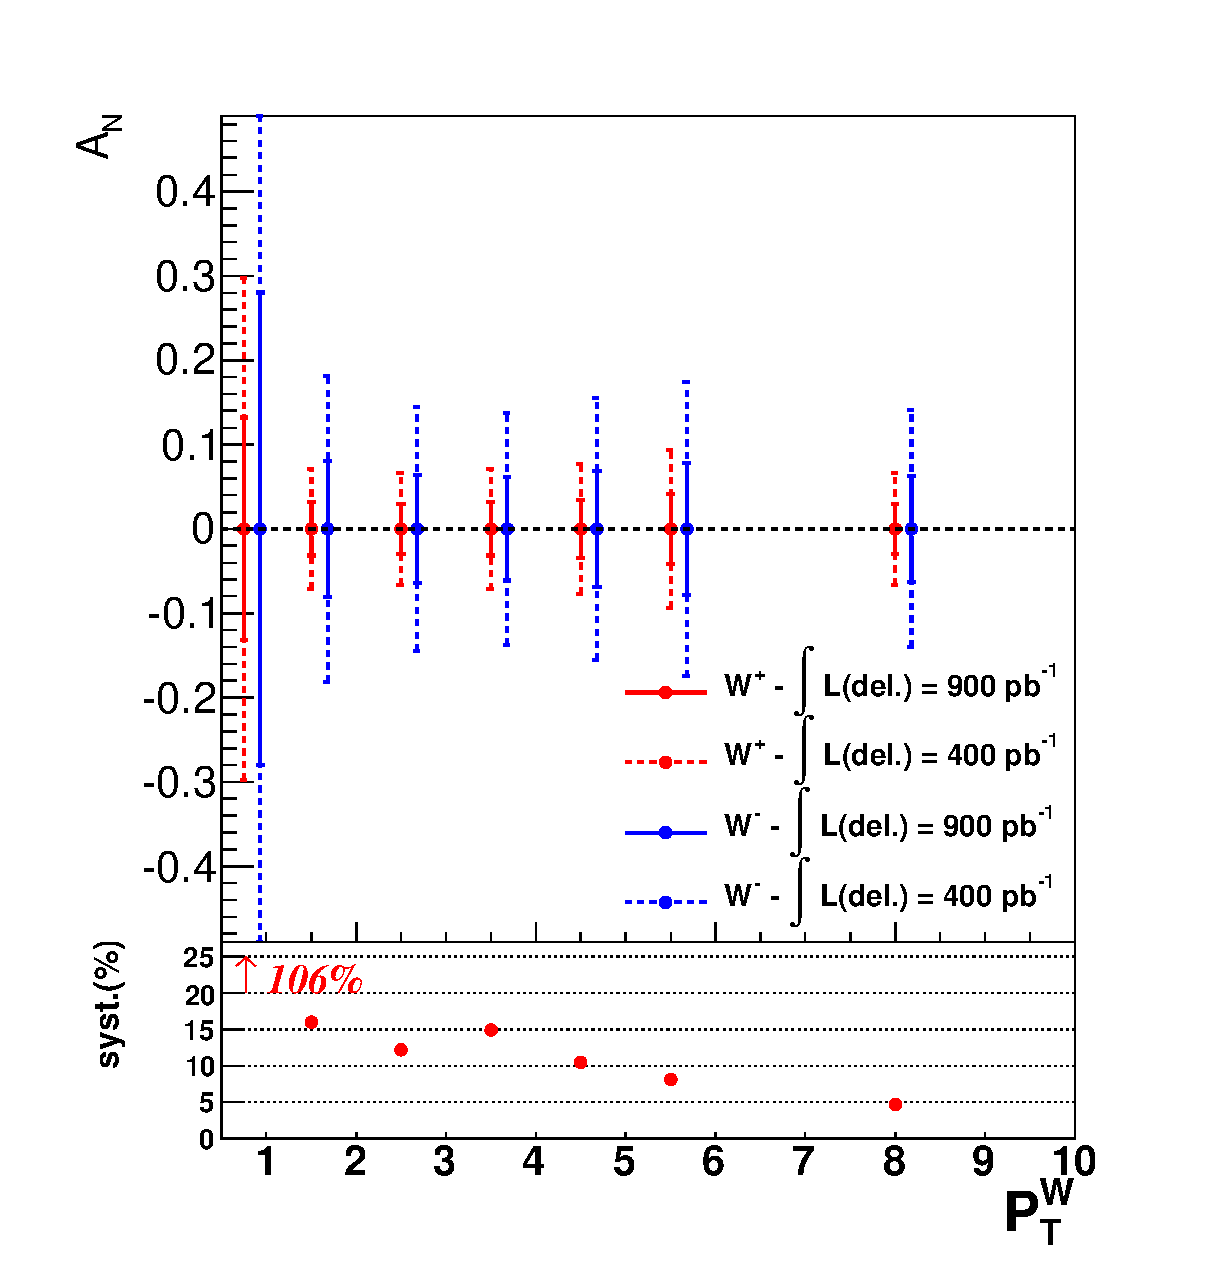
\includegraphics[width=0.32\textwidth]{images/projections/hd_WAsym2016ProjPt_zoom.eps}
  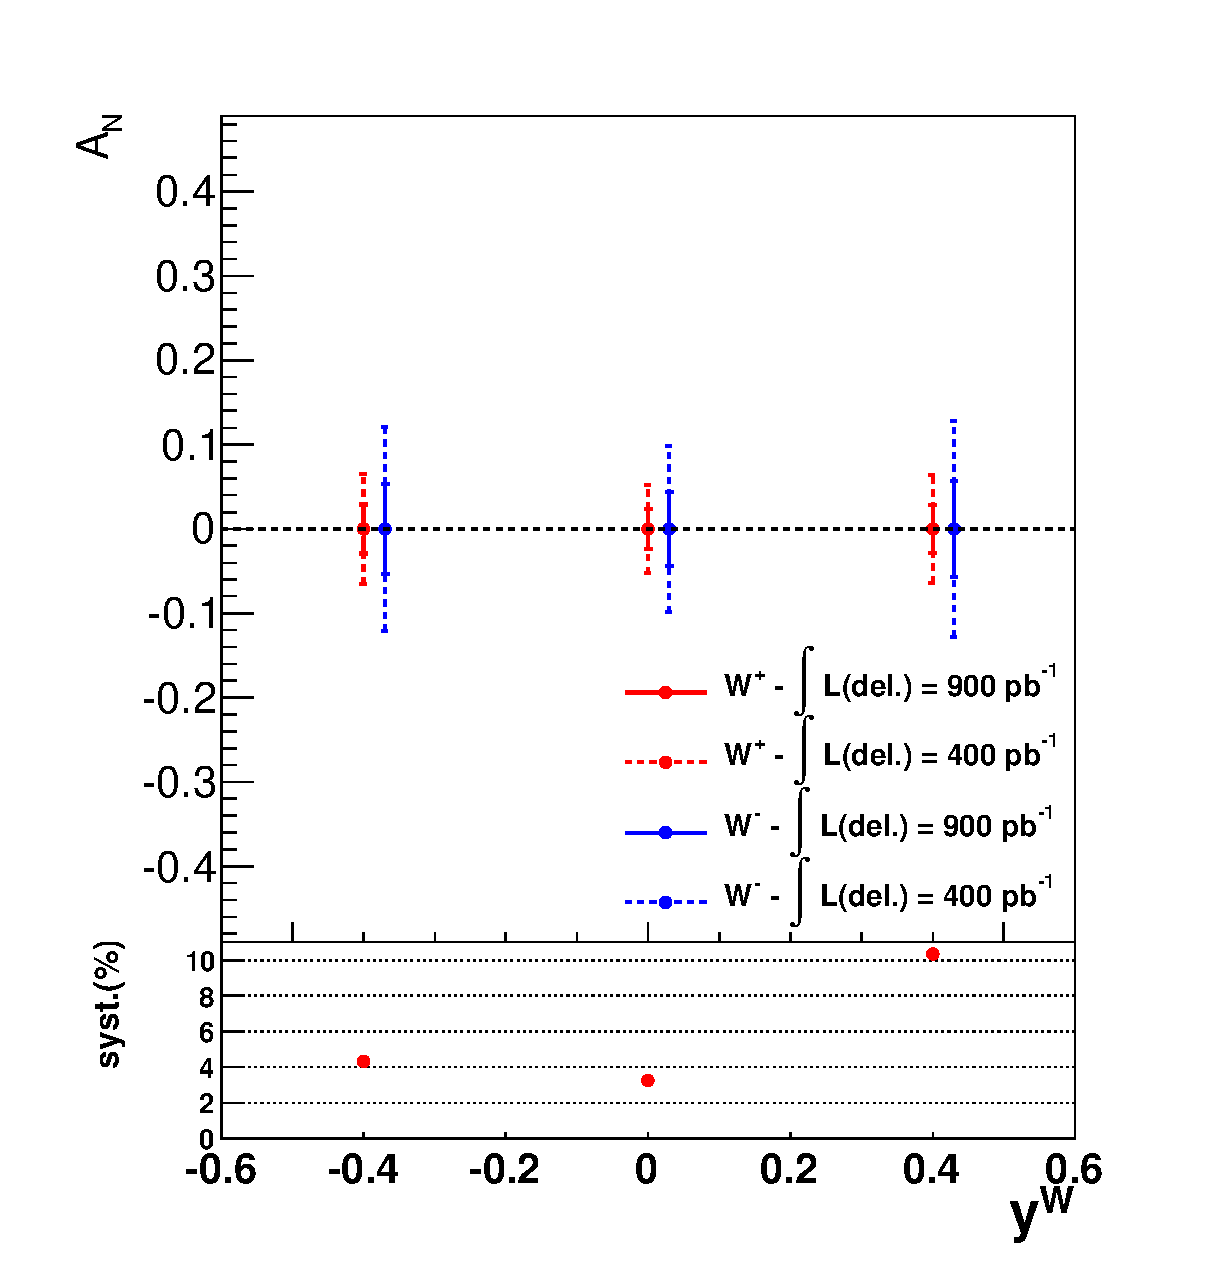
\includegraphics[width=0.32\textwidth]{images/projections/hd_WAsym2016ProjRap_zoom.eps}
  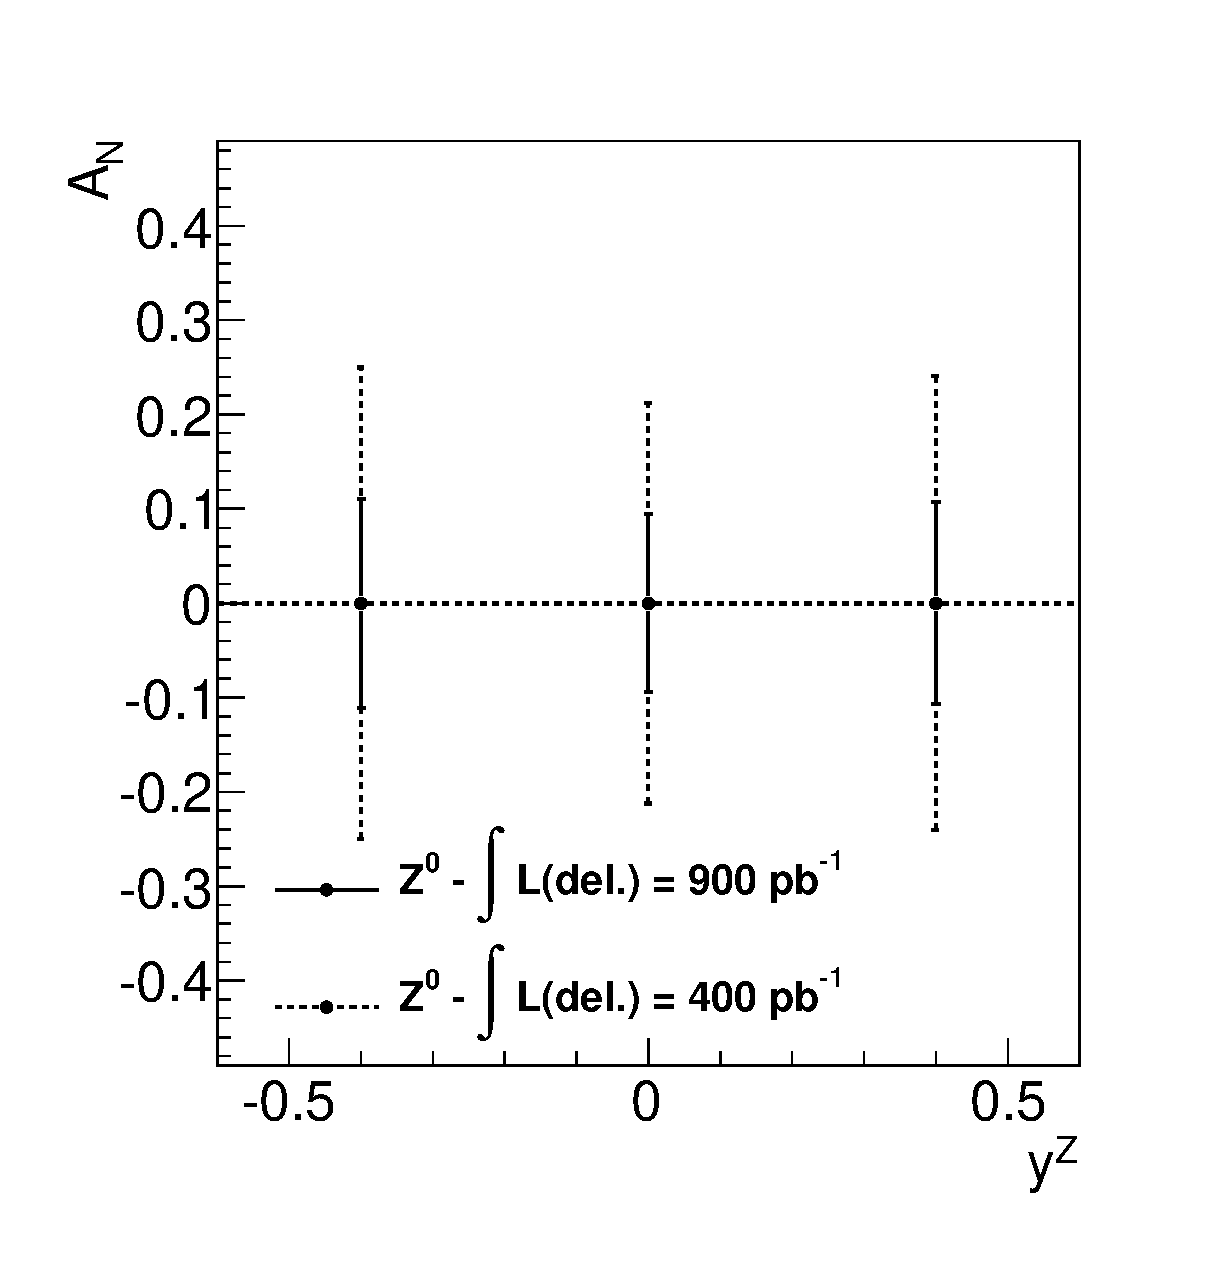
\includegraphics[width=0.32\textwidth]{images/projections/hd_Z0Asym2016ProjRap.eps}
  \caption{Projections of statistical uncertainties of an $A_{N}$ measurement for  $W^{\pm}$ and $Z^{0}$ boson production at STAR assuming a delivered luminosity of 900~$\text{pb}^{-1}$, the 400~$\text{pb}^{-1}$ case is also shown for comparison.}
  \label{Fig:Run16Proj}
\end{figure}
  
%\section{Correction for Background}
%{{{

%In this analysis an optimal set of cuts is applied to select signal enriched
%events without significant loss in the final statistics. The final yields
%include some fraction of background events $f_B$ which along with the signal
%asymmetry contribute to the measured asymmetry $A_N$. In order to extract the
%signal asymmetry we decompose $A_N$ as following:
%
%\begin{equation}
%A_N = f_\text{sig} A^\text{sig}_N + f_B A^B_N,
%\label{eq:asym_bkg}
%\end{equation}
%
%with $f_\text{sig} = 1 - f_B$. The last term in \eqref{eq:asym_bkg} may include
%contributions from various backgrounds which will be discussed later. The
%background fractions and asymmetries have to be estimated in order to extract
%the final asymmetry of the signal:
%
%\begin{equation}
%A^\text{sig}_N = \frac{A_N + f_B A^B_N}{1 - f_B}
%\label{eq_bkg_corr}
%\end{equation}

%}}}


%\section{Sivers Sign Change Extraction}
%{{{

%A binned likelihood method can be used to check the sensitivity of our data to
%the sign of the Sivers function. A direct way of doing this is to compare the
%measured asymmetry \eqref{eq:asym_sqrt} with background corrected expectations
%from \eqref{eq:asym_bkg}. The signal asymmetry $A^\text{sig}_N$ in this case
%directly comes from the model predictions~\eqref{eq:asym_wboson} or
%\eqref{eq:asym_lepton}. The simplest likelihood function can be constructed as a
%product of gaussian terms over all bins:
%
%\begin{equation}
%L = \prod\limits_i G(A_{N,i}, \sigma_{A_{N,i}}; A^\text{sig}_{N,i}).
%\end{equation}
%
%Alternatively, the Sivers sign can be extracted from the Poisson probabilities
%of measured given the expected yields.
%
%\begin{equation}
%L = \prod\limits_{i,\uparrow,\downarrow} P(N_i; N^\text{sig}_{i} + B_i).
%\end{equation}
%
%While this method is more ``classic'' it requires the explicit knowledge of
%luminosity, unpolarized cross section, and efficiencies. These values are
%needed to calculate the expected number of events using \eqref{eq:yield}. The
%two methods are expected to give consistent results. However, the difference
%can be more perceptible when systematic effects are taken into account.

%}}}


%\section{Asymmetry measurement}
%{{{

%For the SSA measurements we are interested in the proton interactions
%$p^{\uparrow/\downarrow} p \to W^\pm \to e^\pm \nu_e$ in which the spin direction of one
%of the protons is irrelevant, \textit{i.e} unpolarized protons. In the
%experiment we can separately measure full and differential cross sections for
%spin-up ($\sigma_\uparrow$), spin-down ($\sigma_\downarrow$), and unpolarized
%($\sigma_0$) interactions which are related as:

%\begin{align}
%\sigma_\uparrow   &= \sigma_0 (1 + A_N ), \\
%\sigma_\downarrow &= \sigma_0 (1 - A_N ).
%\end{align}

%In the following we assume that the polarization vector does not significantly
%deviate from the vertical direction given by the normal unit vector $\vec n$
%along the vertical $y$ axis so, the notation is $P \equiv \vec{P} \cdot
%\vec{n}$. We also assume the same magnitude of the polarization vector for
%spin-up and spin-down bunches, \textit{i.e.} $P = P_\uparrow = P_\downarrow$.
%For unpolarized cross section $\sigma_0 \equiv (\sigma_\uparrow +
%\sigma_\downarrow)/2$ the asymmetry $A_N$ is expressed as:

%\begin{align}
%\label{eq_anapower}
%A_N &= \frac{\sigma_\uparrow - \sigma_\downarrow}{\sigma_\uparrow +
%   \sigma_\downarrow}.
%\end{align}

%The number of recorded events in which the particle is produced with momentum
%$p_T$ at angle $\Omega$ is:

%\begin{align}
%\frac{dN_{\uparrow/\downarrow}}{d\Omega dp_T}(\Omega, p_T) &=
%   {\cal L}_{\uparrow/\downarrow} \frac{d\sigma_0}{d\Omega dp_T}(\Omega, p_T)
%   \varepsilon(\Omega, p_T) \big( 1 \pm A_N(\Omega, p_T) P \big),
%\label{eq:yield_diff}
%\end{align}

%\noindent
%where detection efficiency $\varepsilon$ does not depend on the spin direction
%of the interacting proton. In fact, individual events can be tagged by the
%nominal spin of colliding protons. We thus can bin all collected data  in four
%bins $N_{\uparrow\uparrow}$, $N_{\uparrow\downarrow}$,
%$N_{\downarrow\uparrow}$, and $N_{\downarrow\downarrow}$. For the SSA
%measurement the polarization of one of the beams is ignored by combining the
%yields with opposite spins, \textit{e.g.}

%\begin{align}
%N_{\uparrow}   \equiv N_{\uparrow0}   &= N_{\uparrow\uparrow}   + R_{\frac{0\uparrow}{0\downarrow}} N_{\uparrow\downarrow},\\
%N_{\downarrow} \equiv N_{\downarrow0} &= N_{\downarrow\uparrow} + R_{\frac{0\uparrow}{0\downarrow}} N_{\downarrow\downarrow},
%\end{align}

%\noindent
%where re-weighting factor $R_{\frac{0\uparrow}{0\downarrow}}$ addresses a
%possible relative difference in the spin-up and spin-down intensities of the
%other beam. Studies have shown that $R_{\frac{0\uparrow}{0\downarrow}} \approx
%1$ with good precision.

%We bin our data sample in three observable variables $\{y, \phi, p_T\}$ with
%center and width of the $i$-th bin being $\{y_i, \phi_i, p_{T,i}\}$ and
%$\{\Delta y_i, \Delta\phi_i, \Delta p_{T,i}\} \equiv \{\Delta\Omega_i\{y_i,
%\Delta\phi_i\}, \Delta p_{T,i}\} \equiv \Delta_i$ respectively. The number of
%events in each bin, $N_i$, is calculated by integrating both sides
%of~\eqref{eq:yield_diff} within the bin:

%\begin{align}
%N_{\uparrow/\downarrow, i} =
%   \int\limits_{\Delta_i} \frac{dN_{\uparrow/\downarrow}}{d\Omega dp_T} d\Omega dp_T.
%\end{align}

%\noindent
%In that bin we assume the average value:

%\begin{align}
%A_{N,i} = \frac{1}{\Delta_i} \int\limits_{\Delta_i} A_N d\Omega dp_T,
%\end{align}

%\noindent
%and similarly for the cross section ($\sigma_{0,i}$) and efficiency
%($\varepsilon_i$). Finally, for the yields in each bin we can write:

%\begin{align}
%N_{\uparrow/\downarrow, i} = {\cal L}_{\uparrow/\downarrow} \sigma_{0,i}
%\varepsilon_i \Delta\Omega_i \Delta p_{T,i} \left( 1 \pm A_{N,i}(\Omega, p_T) P \right)
%\label{eq:yield}
%\end{align}

%The spacial distributions of the physical asymmetry and the cross sections are
%the same for the spin-up and spin-down interactions with respect to the spin
%direction. We can use this fact to easily get rid of the  quantities of no
%interest in \eqref{eq:yield}. This is achieved by constructing geometric
%means $\sqrt{N_\uparrow(\phi_i)N_\downarrow(\phi_i+\pi)}$ and
%$\sqrt{N_\uparrow(\phi_i+\pi)N_\downarrow(\phi_i)}$ of the yields


%\begin{align}
%N_\uparrow(\phi_i)       &= {\cal L_\uparrow}
%   \sigma_{0}(\phi_i) \varepsilon(\phi_i)    \Delta\Omega_i \Delta p_T \left( 1 + A_{N}(\phi_i) P \right) \\
%
%N_\uparrow(\phi_i+\pi)       &= {\cal L_\uparrow}
%   \sigma_{0}(\phi_i+\pi) \varepsilon(\phi_i+\pi)    \Delta\Omega_i \Delta p_T \left( 1 + A_{N}(\phi_i+\pi) P \right)
%\end{align}


%\begin{align}
%N_\downarrow(\phi_i+\pi) &= {\cal L_\downarrow}
%   \sigma_{0}(\phi_i+\pi) \varepsilon(\phi_i+\pi) \Delta\Omega_i \Delta p_T \left( 1 - A_{N}(\phi_i+\pi) P \right) \\
%
%N_\downarrow(\phi_i) &= {\cal L_\downarrow}
%   \sigma_{0}(\phi_i) \varepsilon(\phi_i) \Delta\Omega_i \Delta p_T \left( 1 - A_{N}(\phi_i) P \right)
%\end{align}


%Using the relations for the asymmetry and cross section $A_{N}(\phi_i+\pi) =
%-A_{N}(\phi_i)$, $\sigma_0(\phi_i+\pi) = \sigma_0(\phi_i)$ we get for $A_N$


%\begin{align}
%A_{N, i} = \frac{1}{P} \frac{%
%\sqrt{N_{\uparrow}(\phi_i)N_{\downarrow}(\phi_i+\pi)} -
%\sqrt{N_{\uparrow}(\phi_i+\pi)N_{\downarrow}(\phi_i)}
%}{%
%\sqrt{N_{\uparrow}(\phi_i)N_{\downarrow}(\phi_i+\pi)} +
%\sqrt{N_{\uparrow}(\phi_i+\pi)N_{\downarrow}(\phi_i)}
%}
%\label{eq:asym_sqrt}
%\end{align}

%}}}


\appendix
\section{Reproduction of results}
The code used for the present analysis is in the CVS repositories at the link
\newline \url{http://www.star.bnl.gov/cgi-bin/protected/cvsweb.cgi/offline/users/fazio/vbasym/}

\subsection{How to check out and build the analysis code}
To check the code out, from the location where the package will be
installed on your machine issue the following command:

\begin{lstlisting}
    cvs co -d vbasym offline/users/fazio/vbasym/
\end{lstlisting}

%The best way to start with the analysis is to clone the latest version of the
%code from the git repository. From the location where the package will be
%installed on your machine issue the following command:

%\begin{lstlisting}
%    git clone git@github.com:plexoos/vbasym.git 
%    cd vbasym 
%    git submodule init 
%    git submodule update 
%\end{lstlisting}

Before you can build and run the program the following environment variables must
be set:

\begin{lstlisting}
    VBASYM_DIR      
\end{lstlisting}  
this variable contains the path to the project directory 
\begin{lstlisting}  
    VBASYM_RESULTS_DIR
\end{lstlisting}
this variable contains the path to the output directory where the results will be put.

The following environment variables are assumed to be set in the standard STAR
session:

\begin{lstlisting}
    STAR_VERSION
    STAR_HOST_SYS
    ROOTSYS
\end{lstlisting}

Example scripts setting up these variables can be found in the ``scripts/''
directory:

\begin{lstlisting}
    scripts/setup.sh
    scripts/setup.csh
\end{lstlisting}

To build the library run a slightly modified ``cons'' command in the terminal

\begin{lstlisting}
    cd $VBASYM_DIR
    cons CXXFLAGS="-m32 -fPIC -pipe -Wall -Woverloaded-virtual -Wno-long-long" \
         EXTRA_CXXFLAGS="-I${OPTSTAR}/include -Icontrib/root-helper" \
         CPPPATH="#:#StRoot:#.sl64_gcc447/include:${ROOTSYS}/include:./contrib/root-helper"
\end{lstlisting}

The binaries are compiled by issuing the following command:

\begin{lstlisting}
    mkdir build
    cd build
    cmake28 .. -DBOOST_ROOT=${OPTSTAR}
    make
\end{lstlisting}

\subsection{How to split the Monte Carlo file lists}
%=======================================

Embedded Monte-Carlo (MC) files relevant for this analysis were produced using PYTHIA
and are stored on the STAR data disks. The file lists are containted in
``\$VBASYM\_DIR/runlists'' with the following format used for their names: ``\texttt{<run
period>\_mc\_<process type>}''. For example, ``run11\_mc\_Wp2enu'' is a file list for
the $W^{+}\rightarrow e\nu$ MC embedded with Run 11 zero bias events.

The list may contain a large number of files. It is convenient, when submitting
a job to *condor*, to split very long lists into several sublists or ``runs". To
split it do:

\begin{lstlisting}
    cd $VBASYM_DIR/runlists/
    split -d -l <# of lines in each sublist> <list name> <list name>_
\end{lstlisting}

For example, executing the command

\begin{lstlisting}
    split -d -l 5 run11_mc_Z02ee run11_mc_Z02ee_
\end{lstlisting}

will split the content of the list ``run11\_mc\_Z02ee'' in many sublist each
containing 5 lines of the original list and numbered in numerical order starting
with 00. In your directory you should see files named:

\begin{lstlisting}
    run11_mc_Z02ee_00
    run11_mc_Z02ee_01
    run11_mc_Z02ee_02
    ...
\end{lstlisting}

Now all you have to do is to create a text file containing the names of this
sublists you just created. For example create the file named

\begin{lstlisting}
    run11_mc_Z02ee_
\end{lstlisting}

and copy in it the list

\begin{lstlisting}
    run11_mc_Z02ee_00
    run11_mc_Z02ee_01
    run11_mc_Z02ee_02
    ...
\end{lstlisting}

Now all what is needed it to submit to condor the file ``run11\_mc\_Z02ee\_''. The
next section explains how to submit to condor.


\subsection{How to produce the analysis ROOT trees}
%======================================

To produce the jet root trees do:

\begin{lstlisting}
    cd $VBASYM_DIR/scripts
    submit_jobs.sh run12_pp_j3 -z -r12 --jets
\end{lstlisting}

Then to produce the analysis root trees do:

\begin{lstlisting}
    submit_jobs.sh run12_pp_j3 -z -r12
\end{lstlisting}

Other examples:

\begin{lstlisting}
    submit_jobs.sh run11_pp_transverse --jets
    submit_jobs.sh run11_pp_transverse
    submit_jobs.sh run11_mc_Wp2enu_ -m --jets
\end{lstlisting}

\subsection{How to check condor jobs output}
%===============================

One can check the output files returned by condor by verifying the ``tralala"
marker in the log files. There should be just one entry per log file:

\begin{lstlisting}
    grep tralala /path/to/log/* > /tmp/check_jobs_tralala &
    diff --suppress-common-lines -y $VBASYM_DIR/runlists/run11_pp_transverse /tmp/check_jobs_tralala
\end{lstlisting}

\subsection{How to produce histograms from ROOT trees}
%=========================================

Various sets of histograms can be produced from the ROOT trees generated with
`stana`. This stage of the analysis is done with the help of `vbana` executable.
One can run

\begin{lstlisting}
    vbana -f run11_pp_transverse
\end{lstlisting}

and on the MC samples:

\begin{lstlisting}
    vbana -f run11_mc_Wp2enu_
\end{lstlisting}

For help with other options run ``vbana -h''.



\section{Run list}
%{{{
The list of STAR runs used in this analysis is the following
\newline
\newline
\noindent 12038078
12038079
12038080
12038081
12038082
12038086
12038087
12038088
12038089
12038092
12038106
12038108
12038115
12042026
12042027
12042028
12042029
12042030
12042033
12042034
12042035
12042036
12043044
12043045
12043046
12043047
12043048
12043049
12043051
12043052
12043053
12043055
12043060
12043065
12043066
12043067
12043068
12043069
12043077
12043078
12043079
12043081
12044023
12044024
12044025
12044026
12044029
12044030
12044031
12044038
12044039
12044040
12044041
12044042
12044043
12044050
12044051
12044052
12044053
12044054
12044055
12044079
12044080
12044088
12044091
12044092
12044093
12044094
12044096
12044097
12044098
12044099
12044100
12044101
12044102
12044103
12045001
12045002
12045004
12045005
12045006
12045011
12045013
12045016
12046035
12046036
12046037
12046038
12046039
12046040
12046041
12046042
12046043
12046046
12046068
12046069
12046070
12046075
12046095
12046097
12046098
12046099
12046100
12046101
12046102
12046103
12046104
12046105
12046106
12046107
12047009
12047011
12047016
12047017
12047018
12047019
12047020
12047021
12049037
12049038
12049042
12049043
12049044
12049067
12049069
12049070
12049071
12050022
12050023
12050024
12050034
12050035
12050037
12050038
12050039
12050040
12050041
12050042
12050044
12050045
12050046
12050047
12050048
12051006
12051007
12051008
12051009
12051010
12051011
12051012
12051013
12051014
12051020
12051021
12051022
12051023
12051024
12051025
12051026
12051027
12051028
12051029
12051030
12051031
12051032
12051033
12051034
12051035
12051036
12051037
12051038
12051052
12051053
12051054
12051055
12051056
12051057
12051059
12051062
12051063
12051064
12051065
12052011
12052012
12052013
12052014
12052018
12052019
12052020
12052021
12052022
12052023
12052024
12052026
12052027
12052028
12052029
12052030
12052031
12052032
12052033
12052034
12052047
12052048
12052049
12052050
12052051
12052054
12053005
12053006
12053007
12053008
12053009
12053010
12053011
12053013
12053031
12053036
12053039
12053040
12053041
12053042
12053043
12053044
12053048
12053049
12053050
12053051
12053052
12053054
12053056
12053057
12053058
12053070
12054013
12054014
12054015
12054016
12054017
12054018
12054019
12054020
12054021
12054022
12054024
12054025
12054026
12054027
12054028
12054029
12054030
12055031
12055034
12055035
12056007
12056008
12056009
12056010
12056011
12056012
12056013
12056014
12056015
12056016
12056017
12056018
12056019
12056020
12057008
12057009
12057010
12057011
12057012
12057013
12057014
12057016
12057017
12057018
12057019
12057020
12057022
12057050
12057051
12057052
12057053
12057054
12057055
12057057
12057058
12057059
12057060
12058001
12058003
12058004
12058005
12058011
12058012
12058013
12058014
12058015
12058016
12058017
12058018
12058019
12058021
12058022
12058024
12058040
12058048
12058049
12058050
12058052
12058054
12058055
12058057
12058058
12059006
12059007
12059008
12059009
12059010
12059011
12059012
12059013
12059016
12059017
12059018
12059019
12059020
12059021
12059024
12059027
12059028
12059029
12059030
12059031
12059035
12059036
12059037
12059038
12059039
12059070
12059071
12059077
12059078
12059079
12059080
12059082
12059083
12059084
12060001
12060004
12060005
12060006
12060007
12060009
12060010
12060011
12060030
12060033
12060034
12060035
12060036
12060037
12060038
12060039
12060040
12060041
12060042
12060043
12060044
12060045
12060046
12060047
12060048
12060049
12060051
12060056
12060058
12060138
12060143
12060144
12060145
12060146
12061006
12061008
12061010
12061011
12061013
12061014
12061015
12061016
12061018
12062011
12062012
12062013
12062014
12062015
12062016
12062017
12062018
12062019
12062021
12062022
12064003
12064005
12064007
12064008
12064010
12064011
12064012
12064013
12064014
12064015
12064016
12064026
12064027
12064028
12064029
12064033
12064034
12064035
12064036
12064040
12064042
12064043
12064044
12064045
12064058
12064059
12064060
12064061
12064062
12064063
12064064
12064065
12064066
12064067
12064068
12064069
12064070
12064071
12064084
12064085
12064086
12064087
12064088
12064090
12065001
12065004
12065006
12065007
12065009
12065011
12065016
12065018
12075019
12075021
12075022
12075024
12075025
12075027
12075028
12075029
12075030
12075031
12075032
12075033
12075034
12075039
12075040
12075041
12075042
12075043
12076002
12076007
12076008
12076009
12076028
12076029
12076031
12076034
12079005
12079026
12079027
12079028
12079030
12079031
12079038
12079039
12079040
12079041
12079042
12079043
12079045
12079046
12079047
12079049
12079050
12080001
12080004
12080010
12080011
12080012
12080017
12080018
12080020
12080052
12080053
12080054
12080055
12080058
12080059
12080062
12080064
12080066
12080067
12080068
12080069
12080070
12081009
12081011
12081012
12081013
12081014
12081015
12081016
12081020
12081021
12081022
12081023
12081024
12081025
12081027
12081050
12081052
12081053
12081055
12081056
12081057
12081069
12081070
12082001
12082002
12082003
12082004
12082005
12082007
12082022
12082023
12082024
12083011
12083012
12083013
12083014
12083016
12083017
12083018
12083019
12083020
12083021
12083022
12083023
12083024
12083045
12083046
12083047
12083050
12083051
12083052
12083053
12083054
12083055
12083056
12083057
12083058
12083059
12083060
12083061
12084004
12084009
12084010
12084011
12084012
12084013
12084014
12084015
12084016
12084017
12084018
12084019
12084020
12084021
12085023
12085024
12085025
12085026
12085027
12085028
12085029
12085030
12085031
12086001
12086002
12086004
12086005
12086006
12086007
12086017
12086019
12086020
12086033
12086034
12086035
12086037
12086038
12086039
12086040
12086041
12086042
12086046
12086047
12087002
12087003
12087004
12087005
12087012
12087023
12087025
12087026
12087027
12087032
12087033
12087034
12087036
12087038
12087045
12087053
12087054
12087080
12087084
12087085
12087095
12087096
12087097
12087098
12087099
12087100
12087101
12087102
12088022
12088026
12088028
12088030
12088031
12088032
12088033
12088034
12088035
12088049
12088050
12088075
12088076
12088077
12088078
12088079
12088080
12088081
12088086
12088087
12088088
12089006
12089008
12089009
12089010
12089011
12089085
12089086
12089087
12089088
12090002
12090003
12090006
12090007
12090009
12090010
12090011
12090017
12090019
12090020
12090021
12090022
12090042
12090043
12090045
12090046
12090047
12090048
12090049
12090050
12090051
12090052
12090053
12090054
12090055
12090060
12091004
12091005
12091006
12091007
12091009
12091010
12091011
12091012
12091013
12091014
12091016
12091017
12091018
12091019
12091021
12091022
12091023
12091041
12091042
12091043
12091044
12091045
12091046
12091047
12091048
12091049
12091051
12091052
12091053
12091054
12092001
12092002
12092003
12092004
12092005
12092020
12092021
12092037
12092038
12092047
12093001
12093002
12093003
12093004
12093005
12093006
12093007
12093008
12093009
12093010
12093011
12093012
12093014
12093023
12093024
12093025
12093030
12093031
12093032
12093033
12093034
12093036
12093037
12093039
12093040
12093041
12093042
12093044
12093049
12093050
12093051
12094009
12094010
12094011
12094012
12094013
12094014
12094015
12094016
12094017
12094018
12094019
12094020
12094021
12094022
12094024
12094025
12094026
12094060
12094061
12094062
12094063
12094064
12094065
12095005
12095006
12095008
12095010
12095011
12095012
12095013
12095021
12095022
12095023
12095038
12095039
12095041
12095042
12095043
12095044
12095045
12095046
12095050
12095052
12095054
12095055
12095056
12095057
12095058
12095059
12095060
12095061
12095063
12096005
12096006
12096014
12096015
12096016
12096017
12096018
12096019
12096020
12096021
12096023
12096024
12096025
12096026
12096027
12096028
12096029
12096030
12096031
12096032
12096033
12096034
12096047
12096048
12096049
12096056
12096057
12096058
12096059
12096060
12096061
12096062
12097002
12097003
12097004
12097007
12097008
12097009
12097010
12097011
12097012
12097013
12097016
12097017
12097018
12097019
12097020
12097021
12097022
12098008
12098009
12098010
12098012
12098013
12098014
12098017
12098018
12098019
12098020
12098021
12098022
12098030
12098031

%}}}


\newpage

\begin{thebibliography}{9}


%\cite{Kang:2009bp}
\bibitem{Kang:2009bp} 
  Z.~-B.~Kang and J.~-W.~Qiu,
  ``Testing the Time-Reversal Modified Universality of the Sivers Function,''
  Phys.\ Rev.\ Lett.\  {\bf 103}, 172001 (2009)
  [arXiv:0903.3629 [hep-ph]].

\bibitem{STAR_W_AL_2009-paper}
M. Aggarwal et al. (STAR), Measurement of the parity-violating longitudinal single-spin asymmetry
for $W^{\pm}$ boson production in polarized proton-proton collisions at $\sqrt{s} = 500$~GeV, 
Phys. Rev. Lett.106, 062002 (2011), 
arXiv:1009.0326 [hep-ex].

\bibitem{STAR_W_AL_2009-note}
J. Balewski, J. Seele, J. Stevens, and O. Grebenyuk, Measurement of the parity-violating longitu-
dinal single-spin asymmetry $A_{L}$ for $W^{+}$ and $W^{-}$ boson production in polarized $\vec{p} + p$ collisions at
$\sqrt{s}=500$~GeV in Run 9 (STAR Note \# 516), (2010).

\bibitem{STAR_W_AL_2012-paper}
L. Adamczyk et al. (STAR), Measurement of longitudinal spin asymmetries for weak boson production in polarized proton-proton collisions at RHIC, 
Phys.Rev.Lett. 113 (2014) 072301, 
arXiv:1404.6880 [nucl-ex]

\bibitem{STAR_W_AL_2012-note}
J. Balewski, J. Stevens, and J. Zhang, Measurement of the parity-violating longitudinal single-spin
asymmetry for weak boson production in polarized proton-proton collisions in Run 11 + 12 at
$\sqrt{s} = 510$~GeV (STAR Note \# 597), (2013).

\bibitem{STAR_W_xSec_2009-paper}
L. Adamczyk et al. (STAR), Measurement of the $W\rightarrow e\nu$ and $Z^{0}/\gamma^{*}\rightarrow e^{+}e^{-}$ 
production cross sections at mid-rapidity in proton-proton collisions at
$\sqrt{s} = 500$~GeV, 
Phys. Rev. D85, 092010 (2012), 
arXiv:1112.2980 [hep-ex].

\bibitem{STAR_W_xSec_2009-note}
J. Stevens, Measurement of the $W\rightarrow e\nu$ and $Z^{0}/\gamma^{*}\rightarrow e^{+}e^{-}$  
Production Cross Sections at Mid-rapidity in Proton-Proton Collisions at
$\sqrt{s}=500$~GeV in Run 9 (STAR Note \# 546), (2011).

\bibitem{RHIC-Pol} 
RHIC Polarimetry Group, RHIC/CAD Accelerator Physics Note, 490 (2013).

\bibitem{sqrtFormula}
B\"{u}ltmann S et al. {\it Phys. Lett. B} {\bf 632} 167 (2006)\\
B\"{u}ltmann S et al. {\it Phys. Lett. B} {\bf 647} 98 (2007)\\
Ohlsen G G and Keaton Jr P W 1973 {\it Nucl. Instr. Meth.} {\bf 109} 41

\bibitem{Kang:2014}
M.~G.~Echevarria, A.~Idilbi, Z.-B.~Kang, I.~Vitev,
{\it Phys. Rev. D} {\bf 89}, 074013 (2014)

\bibitem{Kang:private}
Z.-B.~Kang, private communication

\bibitem{E866}
E.~A.~Hawker et al. {\it Phys. Rev. Lett.} {\bf 80}, 3715 (1998)

\bibitem{beta_squeeze}
D.~Trbojevic, J.~Yichao, Y.~Luo, BNL-102458-2013-CP
\end{thebibliography}

\end{document}
